\documentclass[12pt,a4paper]{article}
\usepackage[utf8]{inputenc}
\usepackage[T1]{fontenc}
\usepackage{amsmath,amssymb,amsthm,mathtools,bm}
\usepackage{microtype}
\usepackage{graphicx}
\usepackage[margin=2.2cm]{geometry}
\usepackage{hyperref}
\usepackage{xurl}
\usepackage{booktabs,longtable,array,multirow,tabularx}
\usepackage{xcolor}
\usepackage{enumitem}
\usepackage{float}
\usepackage{fancyhdr}
\usepackage{appendix}
\usepackage{caption}
\usepackage{subcaption}

\hypersetup{colorlinks=true,linkcolor=blue!60!black,citecolor=green!50!black,urlcolor=blue!70!black}
\setlength{\headheight}{14.5pt}
\setlength{\emergencystretch}{2em}
\pdfstringdefDisableCommands{%
  \def\SigH{Sigma_H}%
  \def\Sig{Sigma}%
  \def\Yp{Y_p}%
  \def\Neff{N_eff}%
  \def\Teff{T_eff}%
  \def\dd{d}%
  \def\GF{G_F}%
  \def\GL{G_L}%
  \def\GR{G_R}%
  \def\sw{sin^2 theta_W}%
}
\pagestyle{fancy}\fancyhf{}
\fancyhead[L]{\small RABBIT Pedagogical Report v2.0}
\fancyhead[R]{\small J.\ Park}
\fancyfoot[C]{\thepage}
\graphicspath{{figures/}}
\setlength{\parskip}{4pt plus 1pt}

\newcommand{\Sig}{\Sigma}
\newcommand{\SigH}{\Sigma_H}
\newcommand{\Yp}{Y_p}
\newcommand{\Neff}{N_{\rm eff}}
\newcommand{\Teff}{T_{\rm eff}}
\newcommand{\FLRW}{\mathrm{FLRW}}
\newcommand{\dd}{\mathrm{d}}
\newcommand{\order}{\mathcal{O}}
\newcommand{\bx}[1]{\boxed{#1}}
\newcommand{\GF}{G_{\rm F}}
\newcommand{\GL}{G_{\rm L}}
\newcommand{\GR}{G_{\rm R}}
\newcommand{\sw}{\sin^2\!\theta_{\rm W}}

\newtheorem{theorem}{Theorem}[section]
\newtheorem{proposition}[theorem]{Proposition}
\newtheorem{corollary}[theorem]{Corollary}
\newtheorem{lemma}[theorem]{Lemma}
\newtheorem{remark}[theorem]{Remark}
\newtheorem{definition}[theorem]{Definition}

\title{\vspace{-1cm}\textbf{RABBIT: Precision Big Bang Nucleosynthesis\\
with Bianchi Type~I Cosmology}\\[10pt]
\large Pedagogical Report: Canonical Type~I Core and Exact-Characteristic Reference Results\\[6pt]
\normalsize Department of Physics \& OMEG Institute, Soongsil University}
\author{Jiwon Park\\\small\texttt{cosmosapjw@soongsil.ac.kr}}
\date{April 2026 --- v2.0}

\begin{document}
\maketitle

\begin{abstract}
\noindent
This report is a technical pedagogical guide to the current Type~I canonical core of RABBIT (\textbf{R}osenbrock \textbf{A}daptive \textbf{BB}N with \textbf{B}ianchi-type \textbf{I}ntegration \textbf{T}oolkit).  The current \texttt{backend="auto"} authority is the SciPy Type~I reference.  JAX tier-1, exact-characteristic, and no-Teff tier-3 surfaces remain explicit bounded backends and are not publication authority.  The historical figures and likelihood tables remain tied to the exact-characteristic reference chain rather than to every public backend equally.

Within that scope, incomplete decoupling is treated in a tiered way rather than by a full anisotropic collision-coupled Boltzmann/QKE solver.  Tier~1 remains the baseline behind the historical exact-characteristic results quoted here.  Current code scope is broader: tier~2 characteristic three-temperature thermodynamics and a bounded no-Teff tier~3 weak-budget ladder are both implemented as canonical JAX surfaces on declared envelopes.  None of these should be confused with a full species-, momentum-, and angle-resolved anisotropic collision closure.

The exact-characteristic reference architecture is mixed rather than fully exact in every neutrino channel: anisotropic stress and weak-rate monopoles are extracted from characteristic transport, while the neutrino energy-density entry in the Hubble sector is closed through the tiered thermodynamic helper.  The stored shear envelope, nonlinear yield response, legacy $\SigH\simeq0.66$ profile crossing, and FLRW PRIMAT comparison are historical diagnostic outputs.  They have not passed the publication programme's B-02--B-05 matched-physics, domain, convergence, and inference gates and therefore are not current science claims.  Current JAX exact-characteristic comparisons are likewise runtime regressions, not independent validation.

The purpose of this document is therefore narrower than a universal ``full collision'' manual and broader than a short methods note: it explains the exact-characteristic reference results that anchor the report, records how those results sit inside the broader current Type~I canonical core, and provides appendices that help a specialist reader or code user trace the underlying physics and software architecture without overstating deferred or candidate extensions.
\end{abstract}

\tableofcontents
\newpage

%======================================================================
%  PART I: FOUNDATIONS
%======================================================================



\part{Foundations}
\section{Introduction}\label{sec:intro}
%======================================================================

Big Bang nucleosynthesis (BBN) is one of the three observational pillars of standard hot big bang cosmology, alongside the cosmic microwave background (CMB) and the Hubble expansion.  The standard calculation assumes a Friedmann--Lema\^itre--Robertson--Walker (FLRW) spacetime and has been developed to sub-percent precision by codes such as PRIMAT \cite{PitrouPRIMAT2021}, \textsc{PArthENoPE} \cite{PArthENoPE2018}, and \textsc{AlterBBN} \cite{AlterBBN2020}.  The predicted primordial helium-4 mass fraction $\Yp$ depends sensitively on the neutron lifetime $\tau_n$, the baryon-to-photon ratio $\eta$, the effective number of neutrino species $\Neff$, and the weak $n \leftrightarrow p$ interconversion rates.

Although the late-time universe is observationally very close to isotropic, that fact does not by itself exclude a significantly more anisotropic expansion history during the MeV era.  In BBN applications the relevant question is therefore not whether anisotropy exists today, but how much shear and anisotropic stress can be present at $T \sim 0.01$--$10\,\mathrm{MeV}$ without spoiling the primordial light-element yields.  The Bianchi classification provides the natural framework for spatially homogeneous but anisotropic cosmologies \cite{WainwrightEllis1997}.  For Type~I, the effect of anisotropy on BBN was first studied by Barrow \cite{Barrow1976}, while neutrino anisotropic stress (Misner viscosity) was incorporated by Rothman and Matzner \cite{RothmanMatzner1982}.  RABBIT currently provides implementation and diagnostic surfaces for this question; a precision BBN constraint remains an open B-01--B-06 objective.

RABBIT exposes a broader Type~I runtime core than the original SciPy-only framing of this report: (i) the SciPy Type~I reference as \texttt{backend="auto"} and number-of-record; (ii) an explicit bounded JAX tier-1 surface using live weak rates on the linearised Type~I transport surface; (iii) explicit exact-characteristic JAX surfaces (\texttt{"jax\_characteristic"} and \texttt{"jax\_characteristic\_tier2"}); and (iv) an explicit no-Teff JAX tier-3 weak-budget surface (\texttt{"jax\_advanced"}).  None is publication authority.  The report figures are historical diagnostics, and no finite-shear constraint is currently promoted.

\subsection{Runtime-scope declaration}

The strongest claims of this document apply to three distinct scope classes.
\begin{enumerate}
\item \textbf{Reference-result chain:} the exact-characteristic Type~I path that underlies the historical figures in this report, namely Type~I geometry, collisionless characteristic transport, live weak rates, Bennett QED thermodynamics, and the PRIMAT AC2024 network.
\item \textbf{Bounded registry-runtime surfaces:} the SciPy reference/fallback path, the JAX tier-1 live-weak surface, the explicit JAX exact-characteristic tier-1/tier-2 surfaces, and the no-Teff JAX tier-3 weak-budget surface, each with a declared metadata and runtime-regression contract but no publication-validation authority.
\item \textbf{Candidate or deferred perimeter:} Class~A / Class~B / tilted extensions, and full anisotropic collision-coupled Boltzmann/QKE closure.
\end{enumerate}

\subsection{Notation and scope guide}

\begin{table}[t]
\centering
\caption{Load-bearing notation used throughout the main production narrative.  The table is deliberately narrow: it lists the symbols that recur across geometry, transport, weak rates, and inference, and fixes their meanings at the report level.}\label{tab:notation}
\begin{tabularx}{0.95\textwidth}{@{}p{0.17\textwidth}X@{}}
\toprule
Symbol & Meaning \\
\midrule
$N=\ln a$ & e-fold time used as the independent variable of the production solve. \\
$\Sigma$ or $\Sigma_+$ & Hubble-normalised shear amplitude.  In the LRS Type~I production path one has $\Sigma_- = 0$. \\
$\Pi_\nu$ or $\Pi_+$ & Hubble-normalised neutrino anisotropic stress extracted from the characteristic rays. \\
$H/H_{\FLRW}$ & Hubble enhancement relative to the FLRW reference at the same plasma temperature. \\
$I_j, J_j, \Theta_j$ & Characteristic-ray energy shift, Jacobian, and per-ray effective temperature variables; explicit state variables on the SciPy reference path and analytic reconstructions on the compact JAX characteristic path. \\
$\tilde f_0(q)$ & Weak-rate-relevant monopole reconstructed from the characteristic rays. \\
$\lambda_{n\to p},\;\lambda_{p\to n}$ & Live weak interconversion rates evaluated from the current monopole and plasma state. \\
$\Neff$ & Effective neutrino-number diagnostic; in the production path this is helper-based rather than a fully anisotropic scattering-closed observable. \\
$\Delta\chi^2_{\rm prof}(\Sigma_H)$ & Profile statistic retained in the historical diagnostic grid; not a current validated constraint. \\
\bottomrule
\end{tabularx}
\end{table}

Figure~\ref{fig:story_chain} summarises the production logic used throughout the rest of the report.

\begin{figure*}[t]
\centering
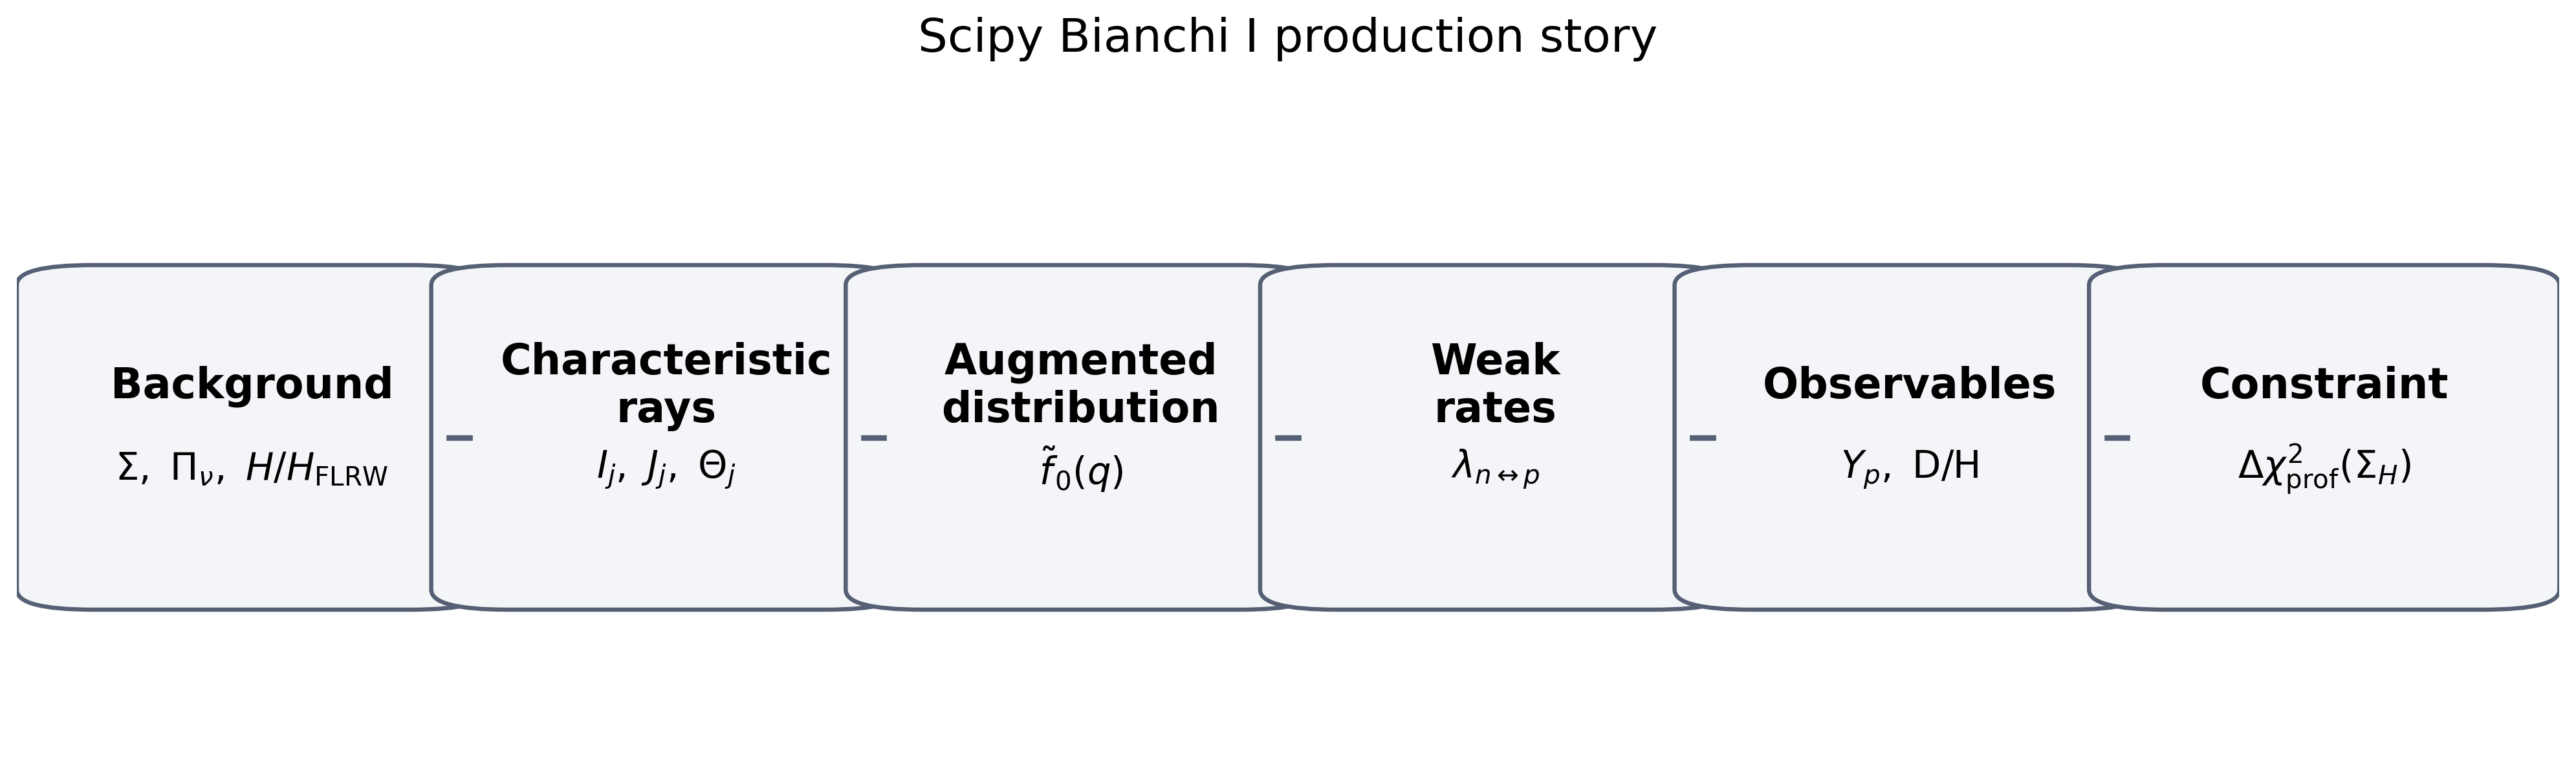
\includegraphics[width=\textwidth]{figures/fig_story_causal_chain.png}
\caption{Historical exact-characteristic diagnostic chain inside the current Type~I runtime core.  The chain runs from geometry through characteristic transport and the augmented monopole to weak rates, BBN observables, and a legacy profile readout.  It is a roadmap for future falsification, not evidence for a current finite-shear constraint.}
\label{fig:story_chain}
\end{figure*}

\subsection{Outline}

Part~I (Foundations) covers the Bianchi geometry (\S\ref{sec:geometry}), collisionless neutrino transport (\S\ref{sec:transport}), the eigenvalue structure (\S\ref{sec:eigenvalues}), a brief historical note on the effective-temperature framework (\S\ref{sec:teff}), and the exact characteristic method (\S\ref{sec:characteristic}).

Part~II (Collision Physics) presents the collision-side scaffolding that is relevant for understanding the tiered incomplete-decoupling story: the collision-integral structure (\S\ref{sec:collision_integral}), the Hannestad--Madsen kernel (\S\ref{sec:hannestad_madsen}), the relaxation-time approximation (\S\ref{sec:rta}), and the incomplete-decoupling hierarchy (\S\ref{sec:incomplete_decoupling}).

Part~III (Production Pipeline) covers weak rates (\S\ref{sec:weak}), the QED equation of state (\S\ref{sec:qed}), the nuclear network (\S\ref{sec:network}), the solver architecture (\S\ref{sec:solver}), the coupled production system (\S\ref{sec:coupled}), results (\S\ref{sec:results}), validation (\S\ref{sec:validation}), discussion (\S\ref{sec:discussion}), and the appendices that supply reference derivations and developer-facing implementation maps.

%======================================================================


\section{Bianchi Type~I Geometry}\label{sec:geometry}
%======================================================================

\subsection{The Wainwright--Hsu Variables}

In the orthonormal-frame approach of Wainwright and Hsu \cite{WainwrightEllis1997}, the LRS (locally rotationally symmetric) Bianchi Type~I spacetime has the metric
\begin{equation}
\dd s^2 = -\dd t^2 + a_1(t)^2\,\dd x^2 + a_2(t)^2\,\dd y^2 + a_3(t)^2\,\dd z^2\,,
\end{equation}
where the mean scale factor is $a = (a_1 a_2 a_3)^{1/3}$ and the mean Hubble rate is $H = \dot{a}/a$.  The shear tensor $\sigma_{ij}$ measures the anisotropic part of the expansion:
\begin{equation}
\sigma_{ij} = \frac{1}{2}(\dot{h}_{ij} - \frac{2}{3}\theta\,h_{ij})\,,
\end{equation}
where $h_{ij}$ is the spatial metric and $\theta = 3H$ is the volume expansion scalar.

The Hubble-normalised shear variables are
\begin{equation}
\Sigma_\pm = \frac{\sigma_\pm}{H}\,,
\end{equation}
with the total shear parameter $\Sigma^2 = \Sigma_+^2 + \Sigma_-^2$.  For LRS symmetry ($\Sigma_- = 0$), the evolution equation is
\begin{equation}
\frac{d\Sigma_+}{dN} = -(2-q)\,\Sigma_+ + \Pi_+\,,\label{eq:dSp}
\end{equation}
where $N = \ln a$ is the e-fold time, $q$ is the deceleration parameter, and $\Pi_+$ is the Hubble-normalised anisotropic stress from free-streaming neutrinos.

For a radiation-dominated universe with equation of state $w = 1/3$, the deceleration parameter is
\begin{equation}
q = 1 + \Sigma^2\,.
\end{equation}
In the FLRW limit ($\Sigma = 0$), $q = 1$ and we recover standard radiation-dominated deceleration.

\subsection{The Friedmann Constraint}

The Friedmann equation in Hubble-normalised form is
\begin{equation}
\Omega = 1 - \Sigma_+^2 - \Sigma_-^2\,,\label{eq:friedmann}
\end{equation}
where $\Omega = \rho/(3H^2)$ is the density parameter.  This is enforced algebraically at each timestep, not as a differential equation.  The physical Hubble rate is then
\begin{equation}
\boxed{H = \frac{H_\FLRW}{\sqrt{1 - \Sigma^2}}\,,}\label{eq:hubble}
\end{equation}
which is enhanced by shear.  For small $\Sigma$ one has $\delta H/H \approx \Sigma^2/2$.  This Hubble enhancement is the first production coupling channel: it accelerates the expansion, shifts weak freeze-out earlier, and raises $\Yp$.

\subsection{Background geometry as the production backbone}

In the present production path the geometry should be read as a coupled geometry--transport system rather than as a prescribed free-decay shear background.  The exact characteristic rays generate a neutrino anisotropic stress $\Pi_\nu$ that feeds back into the shear equation, and the resulting geometry then enters the Hubble rate, the weak rates, and finally the network evolution.  Figure~\ref{fig:story_background} therefore replaces the older mixed production/surrogate summary as the main geometry figure of this report.

\begin{figure*}[t]
\centering
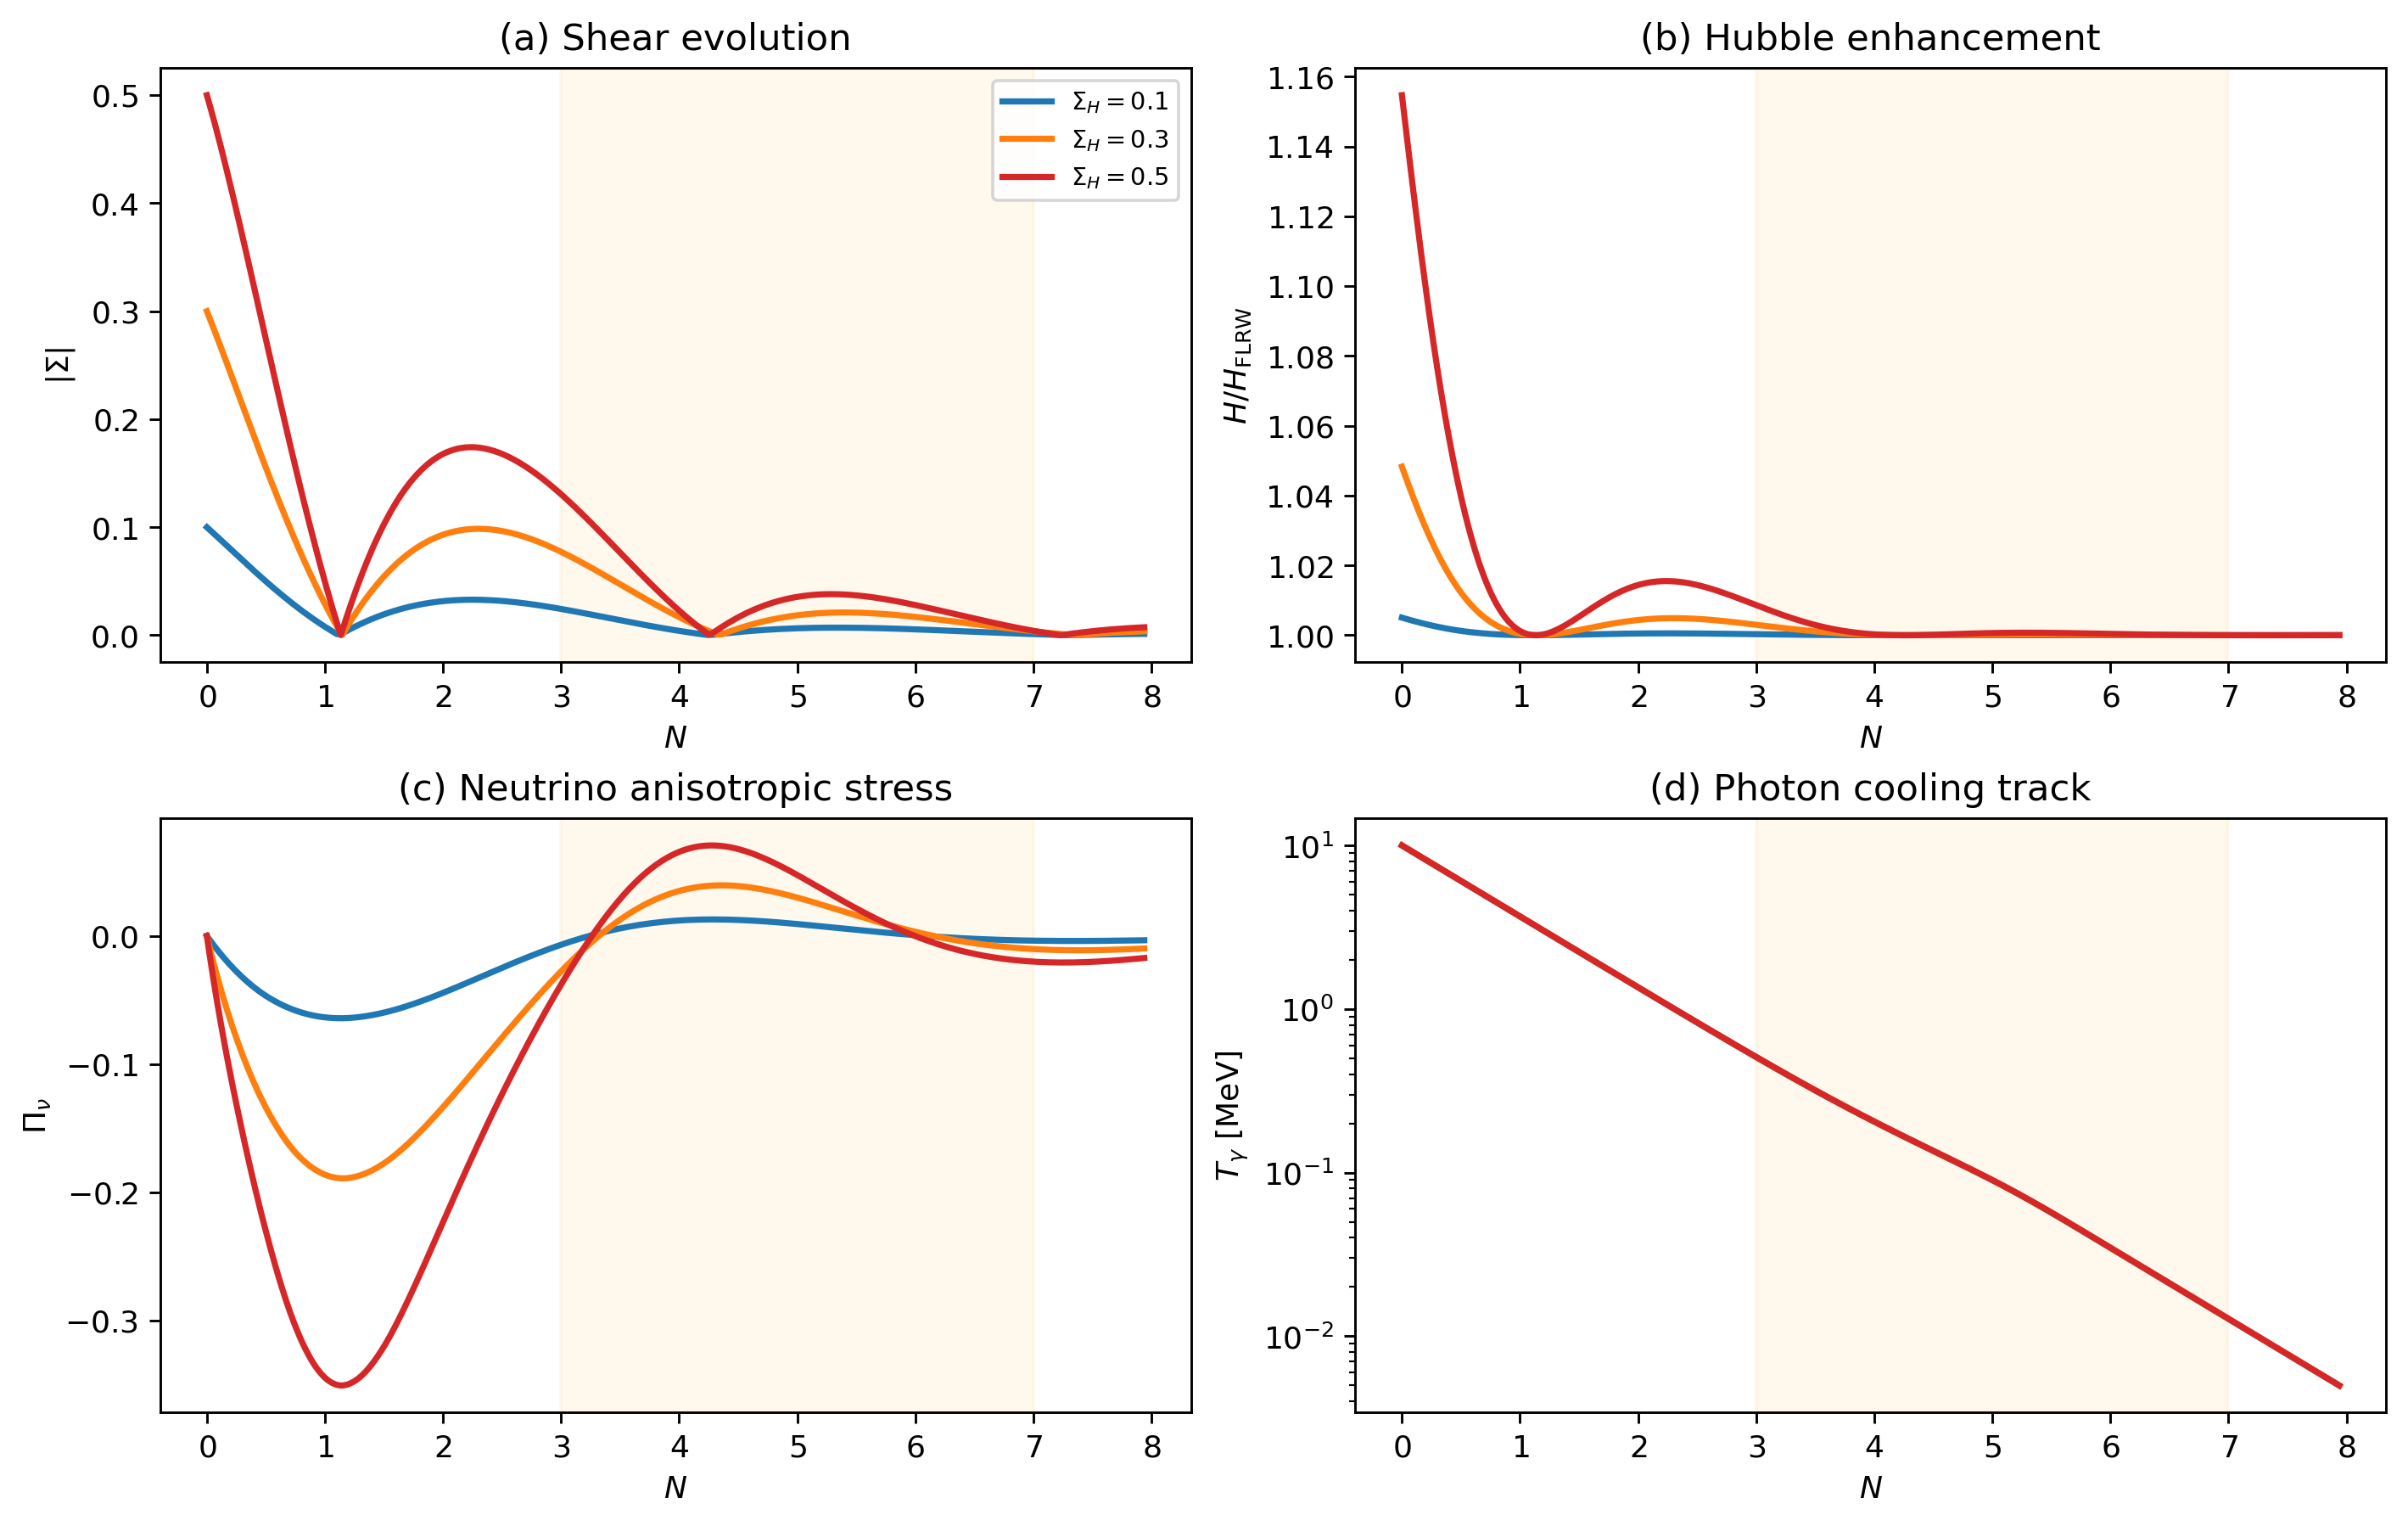
\includegraphics[width=\textwidth]{figures/fig_story_background_geometry.png}
\caption{Background geometry and cosmological evolution along the exact-characteristic reference chain.  Panels show the shear amplitude $|\Sigma|$, the Hubble enhancement $H/H_{\FLRW}$, the neutrino anisotropic stress $\Pi_\nu$, and the photon cooling track $T_\gamma(N)$ for representative initial anisotropies $\Sigma_H=0.1,0.3,0.5$.  The shaded interval marks the BBN-sensitive e-fold range.  The important point is that the geometry is not a featureless free-decay background: the characteristic neutrino sector generates a transient stress backreaction that shapes both the shear history and the expansion rate before the solution relaxes toward the FLRW attractor.}
\label{fig:story_background}
\end{figure*}

The self-consistent characteristic solution therefore differs qualitatively from the older picture in which the geometry is treated as a one-way input to the weak sector.  In the production chain the ordering is instead
\begin{equation}
(\Sigma,\Pi_\nu,H/H_{\FLRW}) \longrightarrow \tilde f_0(q) \longrightarrow (\lambda_{n\to p},\lambda_{p\to n}) \longrightarrow (\Yp,\mathrm{D/H})\,.
\end{equation}
This coupled ordering is the reason the geometry section belongs in the main production narrative rather than being relegated to a purely formal prelude.

%======================================================================


\section{Neutrino Transport: Linearised PSTF Hierarchy}\label{sec:transport}
%======================================================================

\subsection{The Boltzmann Equation in Bianchi Type~I}

The Boltzmann equation for massless neutrinos in a Bianchi Type~I background takes the form
\begin{equation}
\frac{\partial f}{\partial t} + \frac{p^i}{p^0}\frac{\partial f}{\partial x^i} - \Gamma^i_{jk}\frac{p^j p^k}{p^0}\frac{\partial f}{\partial p^i} = \frac{C[f]}{p^0}\,,\label{eq:boltzmann_general}
\end{equation}
where $f(x^i, p^j, t)$ is the one-particle distribution function, $\Gamma^i_{jk}$ are Christoffel symbols of the spatially homogeneous metric, and $C[f]$ is the collision integral.  For spatially homogeneous distributions, the $\partial f/\partial x^i$ term vanishes.

In the fixed dimensionless momentum label $u \equiv ap/T_{\nu,\ast}$ (where $T_{\nu,\ast}$ is a fixed reference neutrino temperature used only to nondimensionalise the momentum), the distribution depends on $u$, the direction cosine $\mu$ with respect to the anisotropy axis, and the e-fold time $N$.  The symbol $u$ is reserved in this report for the transport bookkeeping variable, whereas physical thermal ratios are written as $y \equiv p/T_\nu$ and the neutron--proton mass gap is denoted by $\Delta_{np} \equiv (m_n-m_p)/m_e$.  The collisionless ($C = 0$) Boltzmann equation becomes
\begin{equation}
\frac{\partial f}{\partial N} + \frac{\dd \ln u}{\dd N}\,u\frac{\partial f}{\partial u} + \frac{\dd\mu}{\dd N}\frac{\partial f}{\partial \mu} = 0\,.\label{eq:boltzmann_N}
\end{equation}

\subsection{The PSTF Multipole Expansion}

The Projected Symmetric Trace-Free (PSTF) formalism expands the distribution function perturbation in Legendre multipoles:
\begin{equation}
f(u, \mu, N) = f_0(u)\bigl[1 + \sum_{\ell=0}^{\infty} \Psi_\ell(u, N)\,P_\ell(\mu)\bigr]\,
\end{equation}
where $f_0(u) = [e^u + 1]^{-1}$ is the equilibrium Fermi--Dirac distribution.

In Bianchi Type~I, the collisionless hierarchy for even multipoles (odd multipoles vanish by symmetry) is
\begin{align}
\frac{d\Psi_0}{dN} &= 0\,,\label{eq:psi0}\\
\frac{d\Psi_2}{dN} &= -\frac{8}{15}\,\Sig_+ - D\,\Psi_2\,,\label{eq:psi2}
\end{align}
where $D = 4$ is a reduced-model damping coefficient used in the regression PSTF surrogate.  It encapsulates an effective drain from the quadrupole sector and should not be confused with the exact collisionless characteristic dynamics.  In pure geometric Type~I free streaming there is no direct $\ell=4$ source from the background itself, so the statement that $\Psi_4 = \Psi_6 = \cdots = 0$ is a consistent geometric-source-free truncation should be read separately from the present damped surrogate closure.  In this report, the PSTF system is retained as a reference model, while the production transport results come from the characteristic method.

The monopole perturbation $\Psi_0 = 0$ in the collisionless regime ($T \lesssim 2\;\mathrm{MeV}$), meaning the angle-averaged distribution remains Fermi--Dirac at the zeroth order in the PSTF expansion.  This statement is \emph{only} true for the momentum-independent $\Psi_0$; the exact monopole $\tilde{f}_0(u)$ acquires $u$-dependent corrections, as we show in \S\ref{sec:characteristic}.

\subsection{Anisotropic Stress Extraction}

The neutrino anisotropic stress feeds back into the geometry through
\begin{equation}
\tilde\pi_s = \frac{\int_0^\infty \dd u\,u^3\,f_0(u)\,\Psi_{s,2}(u)}{\int_0^\infty \dd u\,u^3\,f_0(u)} \,\qquad \Pi_+ = 6\,f_\nu\,\bar{\tilde\pi}\,,\label{eq:stress}
\end{equation}
where $s$ indexes the six neutrino species ($\nu_e, \bar\nu_e, \nu_\mu, \bar\nu_\mu, \nu_\tau, \bar\nu_\tau$), $\bar{\tilde\pi}$ is the species-averaged anisotropic stress, and $f_\nu \approx 0.4052$ is the neutrino energy fraction:
\begin{equation}
f_\nu = \frac{\rho_\nu}{\rho_{\rm rad}} = \frac{N_\nu \cdot \frac{7}{8}\left(\frac{4}{11}\right)^{4/3}}{1 + N_\nu \cdot \frac{7}{8}\left(\frac{4}{11}\right)^{4/3}}\,.
\end{equation}

In the linearised PSTF framework, $\Psi_2$ is momentum-independent, so $\tilde\pi = \Psi_2$ and the total DOF count is $6 \times 2 \times N_q = 960$ at $N_q = 80$ momentum grid points (factor 2 for $\Psi_0$ and $\Psi_2$ per species per momentum node, though in practice $\Psi_0 = 0$ reduces this).

%======================================================================


\section{Eigenvalue Structure}\label{sec:eigenvalues}
%======================================================================

\subsection{\texorpdfstring{The Coupled $(\Sig, \tilde\pi)$ Reduced System}{The Coupled (Sigma, pi-tilde) Reduced System}}

In the linearised regime, Eqs.~\eqref{eq:dSp} and \eqref{eq:psi2} (with $\tilde\pi = \Psi_2$) couple to form a $2 \times 2$ autonomous system:
\begin{equation}
\frac{d}{dN}\begin{pmatrix} \Sig_+ \\ \tilde\pi \end{pmatrix} = \underbrace{\begin{pmatrix} -1 & C_{\rm fb}\,f_\nu \\ C_{\rm src} & -C_{\rm drain} \end{pmatrix}}_{\mathbf{M}} \begin{pmatrix} \Sig_+ \\ \tilde\pi \end{pmatrix},\label{eq:matrix}
\end{equation}
where the coupling constants are:
\begin{align}
C_{\rm fb} &= \frac{24}{5} = 4.8 && \text{(feedback: } \Pi_+ = 6f_\nu\tilde\pi \text{ into geometry)}\,,\\
C_{\rm src} &= \frac{8}{15} \approx 0.533 && \text{(source: shear drives quadrupole)}\,,\\
C_{\rm drain} &= D = 4 && \text{(damping of quadrupole by free-streaming)}\,.
\end{align}

\begin{proposition}[Canonical eigenvalues]\label{prop:eigenvalues}
For $f_\nu = 0.4052$ (three active neutrino species with standard thermal history):
\begin{equation}
\bx{\lambda_{\rm slow} = -0.687\,,\qquad \lambda_{\rm fast} = -4.313\,,\qquad \mathrm{tr}(\mathbf{M}) = -5\;\text{(universal).}}
\end{equation}
\end{proposition}

\begin{proof}
The trace is $\mathrm{tr}(\mathbf{M}) = -1 + (-4) = -5$, independent of $f_\nu$.  The determinant is
\begin{equation}
\det(\mathbf{M}) = (-1)(-4) - C_{\rm fb}\,f_\nu \cdot C_{\rm src} = 4 - \frac{24}{5}\cdot\frac{8}{15}\cdot f_\nu = 4 - \frac{192}{75}\,f_\nu\,.
\end{equation}
For $f_\nu = 0.4052$:
\begin{equation}
\det(\mathbf{M}) = 4 - 2.560 \times 0.4052 = 4 - 1.037 = 2.963\,.
\end{equation}
The discriminant is
\begin{equation}
\Delta = \mathrm{tr}^2 - 4\det = 25 - 4(2.963) = 25 - 11.852 = 13.148 > 0\,,
\end{equation}
so both eigenvalues are real:
\begin{equation}
\lambda = \frac{-5 \pm \sqrt{13.148}}{2} = \frac{-5 \pm 3.626}{2}\,.
\end{equation}
This gives $\lambda_{\rm slow} = (-5 + 3.626)/2 = -0.687$ and $\lambda_{\rm fast} = (-5 - 3.626)/2 = -4.313$.
\end{proof}

\begin{remark}[The $-0.617$ error]
An earlier version of this report stated $\lambda_{\rm slow} = -0.617$.  That value requires $f_\nu = 0.506$, which is not physically realised in the Standard Model with three active neutrino species.  The correct value is $\lambda_{\rm slow} = -0.687$ with $f_\nu = 0.4052$.  The value $-0.617$ is \textbf{retired} and should not be used.
\end{remark}

\subsection{The Transport Eigenvalues: Complex Oscillatory Decay}

The reduced $(\Sig, \tilde\pi)$ system of \eqref{eq:matrix} uses a renormalised anisotropic stress variable $\tilde\pi$.  To expose the oscillatory structure, we return to the original $(\Sig, \Psi_2)$ variables.  The collisionless PSTF hierarchy closes at $\ell = 2$ for Type~I, giving two equations without quadrupole damping:
\begin{align}
\frac{\dd\Sig}{\dd N} &= -\Sig + \Pi\,,\qquad \Pi = 6\,f_\nu\,\Psi_2\,,\label{eq:dSig_tr}\\
\frac{\dd\Psi_2}{\dd N} &= -\frac{8}{15}\,\Sig\,.\label{eq:dPsi2_tr}
\end{align}
Note the critical sign: shear \emph{sources} a \emph{negative} quadrupole perturbation (an opposing anisotropic stress), and the positive-definite feedback coefficient $6f_\nu$ converts this to a \emph{negative} $\Pi$.  The $2\times 2$ matrix in the $(\Sig, \Psi_2)$ basis is
\begin{equation}
\mathbf{M}_{\rm tr} = \begin{pmatrix} -1 & 6\,f_\nu \\ -8/15 & 0 \end{pmatrix}\,.\label{eq:Mtr}
\end{equation}
This differs from the reduced system \eqref{eq:matrix} in two ways: (i)~the off-diagonal entries have \emph{opposite} signs (negative feedback loop), and (ii)~there is no quadrupole damping ($M_{22} = 0$).  The trace is $\mathrm{tr}(\mathbf{M}_{\rm tr}) = -1$ and the determinant is
\begin{equation}
\det(\mathbf{M}_{\rm tr}) = 0 - (6f_\nu)\!\left(-\frac{8}{15}\right) = \frac{16\,f_\nu}{5}\,.
\end{equation}
The discriminant is $\Delta = 1 - 4 \times 16f_\nu/5 = 1 - 64f_\nu/5$.  For $f_\nu > 5/64 \approx 0.078$ (always satisfied for $N_\nu \geq 1$), $\Delta < 0$ and the eigenvalues are complex:
\begin{equation}
\bx{\lambda = -\frac{1}{2} \pm i\omega\,,\qquad \omega = \frac{1}{2}\sqrt{\frac{64 f_\nu}{5} - 1} \approx 1.023\;\text{rad/e-fold}\,.}
\end{equation}

\begin{corollary}[Self-consistent decay law]
The real part $\mathrm{Re}(\lambda) = -\mathrm{tr}/2 = -1/2$ is exact and $f_\nu$-independent.  The physical shear decays as
\begin{equation}
\bx{|\Sig(N)| \sim e^{-N/2}\,,\qquad \sigma \propto a^{-5/2}\,,}
\end{equation}
with damped oscillations of frequency $\omega \approx 1.023\;\mathrm{rad/e\text{-}fold}$.
\end{corollary}

\begin{remark}[Relationship between the two eigenvalue systems]
The reduced system \eqref{eq:matrix} and the transport system \eqref{eq:Mtr} describe the same physics at different levels of approximation.  The transport system uses the bare PSTF variables $(\Sig, \Psi_2)$ without damping and exhibits the physically observed oscillatory decay ($\sigma \propto a^{-5/2}$).  The reduced system uses the energy-weighted stress variable $\tilde\pi$ with a Markovian quadrupole damping $D = 4$ that models the decorrelation from free-streaming.  This damping converts the oscillatory dynamics into overdamped decay ($\lambda_{\rm slow} = -0.687$, $\lambda_{\rm fast} = -4.313$, both real).  The two systems are \emph{not} related by a simple variable rescaling: the $D = 4$ closure adds qualitatively new dissipation.  Both descriptions are useful: the transport eigenvalues give the correct oscillation envelope ($\sigma \propto a^{-5/2}$), while the reduced eigenvalues characterise the effective decay rate of the slow mode after the fast transient has died away.
\end{remark}

This is significantly slower than the free decay $\sigma \propto a^{-3}$ (eigenvalue $-1$), which obtains when neutrino free-streaming is neglected.  The physical origin: free-streaming neutrinos store shear energy in their quadrupole moment $\Psi_2$, creating a viscous reservoir that releases energy back to the geometry on the timescale $|\lambda_{\rm slow}|^{-1} \approx 1.46$ e-folds.

As a historical scale illustration only, extrapolating the deprecated diagnostic crossing near $\SigH=0.66$ with $a^{-3}$ or $a^{-5/2}$ changes the resulting present-day order of magnitude by roughly four decades.  Because the starting crossing is not a validated BBN constraint, neither extrapolated number is a current science result.

\subsection{Eigenvector Structure and Mode Mixing}

The eigenvectors of $\mathbf{M}$ reveal the physical content of each mode.  For the slow mode ($\lambda_{\rm slow} = -0.687$), the eigenvector is
\begin{equation}
\mathbf{v}_{\rm slow} = \begin{pmatrix} 1 \\ C_{\rm src}/(\lambda_{\rm slow} + C_{\rm drain}) \end{pmatrix} = \begin{pmatrix} 1 \\ (8/15)/(4 - 0.687) \end{pmatrix} = \begin{pmatrix} 1 \\ 0.161 \end{pmatrix}\,,
\end{equation}
indicating that the slow mode is predominantly shear with a small quadrupole component ($\tilde\pi/\Sig \approx 0.16$).  The fast mode ($\lambda_{\rm fast} = -4.313$) has eigenvector
\begin{equation}
\mathbf{v}_{\rm fast} = \begin{pmatrix} 1 \\ C_{\rm src}/(\lambda_{\rm fast} + C_{\rm drain}) \end{pmatrix} = \begin{pmatrix} 1 \\ (8/15)/(4 - 4.313) \end{pmatrix} = \begin{pmatrix} 1 \\ -1.70 \end{pmatrix}\,.
\end{equation}
The fast mode has $|\tilde\pi| > |\Sig|$: it is a quadrupole-dominated oscillation that decays within $\sim$1 e-fold.

Given generic initial conditions $\Sig(0) = \Sig_0$, $\tilde\pi(0) = 0$ (no initial anisotropic stress), the decomposition is:
\begin{equation}
\begin{pmatrix} \Sig(N) \\ \tilde\pi(N) \end{pmatrix} = A_{\rm s}\,\mathbf{v}_{\rm slow}\,e^{\lambda_{\rm slow} N} + A_{\rm f}\,\mathbf{v}_{\rm fast}\,e^{\lambda_{\rm fast} N}\,,
\end{equation}
where $A_{\rm s}$ and $A_{\rm f}$ are determined by the initial conditions.  For $\tilde\pi(0) = 0$:
\begin{equation}
A_{\rm s} = \frac{v_{2,\rm fast}}{v_{2,\rm fast} - v_{2,\rm slow}}\,\Sig_0 \approx 0.914\,\Sig_0\,,\qquad A_{\rm f} = \frac{-v_{2,\rm slow}}{v_{2,\rm fast} - v_{2,\rm slow}}\,\Sig_0 \approx 0.086\,\Sig_0\,.
\end{equation}
Thus $\sim$91.4\% of the initial shear enters the slow mode and only $\sim$8.6\% enters the fast mode.  After $N \sim 2$ e-folds, the fast mode has decayed by $e^{-4.313 \times 2} \approx 2 \times 10^{-4}$ and only the slow mode survives.

\subsection{Physical Interpretation: The Neutrino Viscous Reservoir}

The slow decay can be understood as an energy storage mechanism.  Free-streaming neutrinos develop an anisotropic stress $\Pi_\nu$ in response to the geometric shear $\Sig$.  This stress acts as a sink for shear kinetic energy, converting it to internal energy of the neutrino distribution (encoded in $\Psi_2$).  However, the stored energy leaks back: the feedback term $C_{\rm fb}\,f_\nu\,\tilde\pi$ in the shear equation \eqref{eq:dSp} returns anisotropic stress to the geometry, slowing the net decay.

The total energy budget satisfies
\begin{equation}
\frac{\dd}{\dd N}(\rho_\sigma + \rho_{\pi}) = -(5 + \text{interaction})\,(\rho_\sigma + \rho_{\pi})\,,
\end{equation}
where $\rho_\sigma \propto \Sig^2$ is the shear energy and $\rho_\pi \propto \tilde\pi^2$ is the quadrupole energy.  The universal trace $\mathrm{tr}(\mathbf{M}) = -5$ sets the total dissipation rate, but the \emph{partition} between shear and quadrupole determines the effective decay constant for each component individually.

\subsection{Sensitivity to the neutrino energy fraction}

The eigenvalues depend on the neutrino energy fraction $f_\nu$, which in turn depends on the number of neutrino species and their thermal history.  The discriminant $\Delta = 25 - 4\det$ vanishes at
\begin{equation}
f_{\nu,\rm crit} = \frac{75}{4 \times 192}\,(25 - 16) = \frac{75 \times 9}{768} = 0.879\,,
\end{equation}
above which the eigenvalues become complex (oscillatory shear decay even in the reduced system).  Since $f_\nu = 0.4052 < 0.879$, the physical case has real eigenvalues.

For hypothetical scenarios with additional light species (e.g.\ sterile neutrinos), $f_\nu$ increases, and the eigenvalue splitting $|\lambda_{\rm slow} - \lambda_{\rm fast}|$ decreases.  At $f_\nu \to 0$ (no neutrinos), $\lambda_{\rm slow} \to -1$ and $\lambda_{\rm fast} \to -4$, recovering the free-decay shear rate and the independent quadrupole damping.

\subsection{Quasi-Static Attractor}

After $\sim$2 e-folds, the stress-to-shear ratio converges to the quasi-static attractor:
\begin{equation}
\frac{|\tilde\pi|}{|\Sig|} \to \frac{C_{\rm src}}{C_{\rm drain}} = \frac{8/15}{4} \approx 0.133\,.
\end{equation}
This attractor ratio determines the effective feedback strength and is insensitive to initial conditions.  Its physical meaning is simple: the quadrupole reaches a quasi-static balance between the source from geometric shear ($C_{\rm src}\,\Sig$) and the damping from free-streaming ($C_{\rm drain}\,\tilde\pi$).

The attractor timescale can be estimated from the fast eigenvalue: $\tau_{\rm att} \sim |\lambda_{\rm fast}|^{-1} \approx 0.23$ e-folds.  After $\sim 5\tau_{\rm att} \approx 1.2$ e-folds, the system is within 1\% of the attractor.

\begin{figure}[t]
\centering
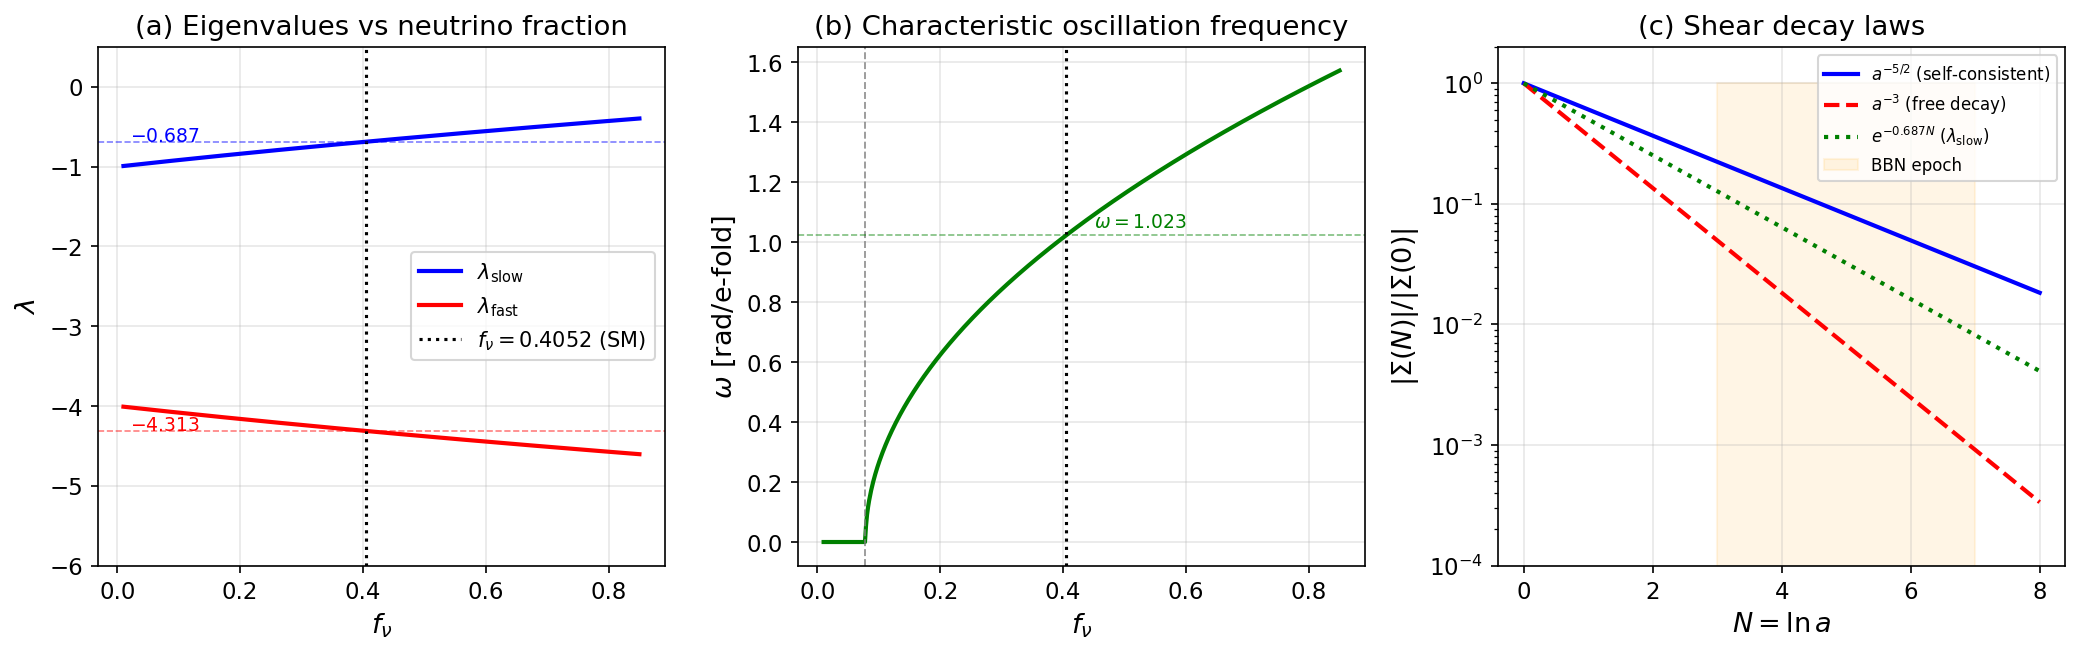
\includegraphics[width=\textwidth]{fig_ped01_eigenvalue_sensitivity.png}
\caption{Eigenvalue structure.  (a)~$\lambda_{\rm slow}$ and $\lambda_{\rm fast}$ as functions of $f_\nu$; the vertical dashed line marks $f_\nu = 0.4052$ (three SM neutrinos), giving $\lambda_{\rm slow} = -0.687$.  (b)~Oscillation frequency $\omega$ of the transport eigenvalues; at $f_\nu = 0.4052$, $\omega = 1.023\;\mathrm{rad/e\text{-}fold}$.  (c)~Shear decay envelopes: self-consistent $a^{-5/2}$ vs free decay $a^{-3}$ vs the slow eigenmode $e^{-0.687 N}$, with the BBN epoch highlighted.}\label{fig:eigenvalues}
\end{figure}

%======================================================================


\section{Effective-Temperature Framework}\label{sec:teff}
%======================================================================

\subsection{Angular Deformation of the Distribution}

In the linearised PSTF framework, the anisotropy can be characterised by an angle-dependent effective temperature:
\begin{equation}
\Theta(\mu) = 1 + T_2\,P_2(\mu)\,,\qquad T_2 = \tilde\pi/4\,,\label{eq:theta_def}
\end{equation}
so that the distribution function takes the form $f(u, \mu) \approx f_{\rm FD}(u/\Theta(\mu))$.  The angle-averaged (monopole) spectrum is then the spectrally hardened integral
\begin{equation}
\tilde{f}_0(u) = \frac{1}{2}\int_{-1}^{1}\dd\mu\;\frac{1}{e^{u/\Theta(\mu)} + 1}\,,\label{eq:teff_mono}
\end{equation}
which is evaluated with $N_\mu = 16$ Gauss--Legendre nodes.

The spectral hardening arises from Jensen\'s inequality: the Fermi--Dirac function is convex, so the average of $f_{\rm FD}(u/\Theta(\mu))$ over $\mu$ differs from $f_{\rm FD}(u)$ at $\order(T_2^2)$.  At leading order, the perturbation is
\begin{equation}
\frac{\delta f}{f_0} = \frac{q\,e^q}{(e^q + 1)}\left(\frac{T_2^2}{5}\cdot\frac{q\,e^q - e^q + 1}{(e^q + 1)}\right) + \order(T_2^3)\,.
\end{equation}
This produces a soft deficit ($\delta f < 0$) at $q \lesssim 2$ and a hard excess ($\delta f > 0$) at $q \gtrsim 2$, shifting the mean neutrino energy upward.

\subsection{Historical limitations of the effective-temperature closure}

The $\Teff$ framework has two fundamental limitations:

\begin{enumerate}
\item \textbf{$q$-independence}: the angular deformation $\Theta(\mu)$ is independent of momentum $q$.  In reality, the energy shift along each direction is momentum-dependent (see \S\ref{sec:characteristic}), producing spectral distortions beyond the $\Teff$ parametrisation.

\item \textbf{Coordinate singularity}: when $T_2 \to -1/2$ (i.e.\ $c_2 = -1$), $\Theta(\mu = 0) \to 0$, causing a singularity in the Fermi--Dirac function.  This is reached for $\SigH \gtrsim 0.25$ and limits the valid parameter range.
\end{enumerate}

Both limitations are resolved by the characteristic method (\S\ref{sec:characteristic}), which replaces the $\Teff$ parametrisation with exact solutions along geodesic rays.

\begin{figure}[t]
\centering

\includegraphics[width=\textwidth]{fig02.png}
\caption{Spectral distortion mechanisms.  (a)~$\Teff$ angular profiles $\Theta(\mu)$ for three values of $\tilde\pi$.  (b)~Perturbative spectral hardening $\delta f/f_0$.  (c)~Exact characteristic monopole shift.}\label{fig:teff}
\end{figure}

%======================================================================


\section{Exact Characteristic Ray Transport}\label{sec:characteristic}
%======================================================================

\subsection{The Method of Characteristics}

The collisionless Boltzmann equation for massless neutrinos in LRS Bianchi Type~I admits an \emph{exact} solution by the method of characteristics.  Each characteristic curve (``ray'') follows a geodesic of the anisotropic spacetime.

The ray direction $\mu$ (cosine of the angle with respect to the anisotropy axis) evolves according to
\begin{equation}
\frac{d\mu}{dN} = 3\Sig_+\,\mu(1 - \mu^2)\,,
\end{equation}
which integrates to the analytic form
\begin{equation}
X(\mu) \equiv \frac{\mu^2}{1 - \mu^2} = X_0\,e^{6S}\,,\qquad S = \int_0^N \Sig_+(N')\,\dd N'\,.\label{eq:X_evolution}
\end{equation}

The energy of a neutrino along ray $j$ shifts by the accumulated integral
\begin{equation}
\frac{dI_j}{dN} = \Sig_+\,P_2(\mu_j)\,,\label{eq:dI}
\end{equation}
so the distribution function is
\begin{equation}
\bx{f(u, \mu_j, N) = f_0\!\left(u\,e^{2I_j(N)}\right) = f_{\rm FD}\!\left(\frac{u}{\Theta_j}\right)\,,\qquad \Theta_j = e^{-2I_j}\,.}\label{eq:char_sol}
\end{equation}

This is an \emph{exact} solution of the collisionless Boltzmann equation: no approximation, no truncation.  Each ray is a Fermi--Dirac distribution with a direction-dependent effective temperature $\Theta_j$.  In code, the same exact physics appears in two numerically different representations: the SciPy reference path stores the explicit ray variables $(I_j, J_j)$ together with the shared accumulated shear $S$, whereas the compact JAX characteristic surface evolves only $S$ and reconstructs $I_j(S)$ and $J_j(S)$ analytically.

\subsection{Geodesic Equations in Bianchi Type~I}

To derive the characteristic solution, we begin from the geodesic equation for massless particles in the LRS Bianchi Type~I metric.  Writing the metric as $\dd s^2 = -\dd t^2 + a_\perp^2(t)(\dd x^2 + \dd y^2) + a_\parallel^2(t)\,\dd z^2$, the Hubble rates in the perpendicular and parallel directions are
\begin{equation}
H_\perp = \frac{\dot{a}_\perp}{a_\perp} = H(1 - \Sig_+)\,,\qquad H_\parallel = \frac{\dot{a}_\parallel}{a_\parallel} = H(1 + 2\Sig_+)\,.
\end{equation}

A massless neutrino with 4-momentum $p^\alpha = (E, p_x, p_y, p_z)$ has $E^2 = p_\perp^2/a_\perp^2 + p_z^2/a_\parallel^2$ (using physical momenta).  Defining the direction cosine $\mu = p_\parallel/(a_\parallel E)$ with respect to the symmetry axis, the geodesic equation gives:
\begin{equation}
\frac{\dd E}{E\,\dd t} = -H - \sigma_+ P_2(\mu)\,,\qquad \frac{\dd\mu}{\dd t} = 3H\sigma_+\,\mu(1-\mu^2)/H = 3\Sig_+\,H\,\mu(1-\mu^2)\,.
\end{equation}

Switching to e-fold time $N = \ln a$:
\begin{align}
\frac{\dd\ln E}{\dd N} &= -1 - \Sig_+\,P_2(\mu)\,,\label{eq:dE_dN}\\
\frac{\dd\mu}{\dd N} &= 3\Sig_+\,\mu(1-\mu^2)\,.\label{eq:dmu_dN}
\end{align}

The fixed transport label $u = Ea/T_0$ then satisfies $\dd\ln u/\dd N = \dd\ln E/\dd N + 1 = -\Sig_+\,P_2(\mu)$.  Defining the energy-shift integral $I(N) = \int_0^N \Sig_+(N')\,P_2(\mu(N'))\,\dd N'$, we have $u_{\rm eff} = u\,e^{2I}$ (the factor 2 arises from the standard normalisation convention for the PSTF quadrupole).

\subsection{Analytic Integration of the Direction Equation}

The direction equation \eqref{eq:dmu_dN} can be integrated analytically.  Define $X = \mu^2/(1-\mu^2)$, so that $\dd X/X = 2\dd\mu/[\mu(1-\mu^2)] = 6\Sig_+\,\dd N$.  Therefore:
\begin{equation}
X(N) = X_0\,e^{6S(N)}\,,\qquad S(N) = \int_0^N \Sig_+(N')\,\dd N'\,,
\end{equation}
and
\begin{equation}
\mu(N) = \frac{\sqrt{X_0\,e^{6S}}}{\sqrt{1 + X_0\,e^{6S}}}\,.
\end{equation}

The angular Jacobian $J_j = \dd\mu_j(0)/\dd\mu_j(N)$ is needed for proper quadrature weighting.  From $X = X_0\,e^{6S}$, we compute:
\begin{equation}
J_j = \frac{\dd\mu_{j,0}}{\dd\mu_j} = \frac{\mu_j(1-\mu_j^2)}{\mu_{j,0}(1-\mu_{j,0}^2)} = \frac{(1-\mu_{j,0}^2)^2}{(1-\mu_j^2)^2}\,e^{-6S}\,.
\end{equation}

This Jacobian accounts for the compression/expansion of solid angle elements as the anisotropic expansion stretches the angular distribution.

\subsection{The Method of Characteristics}

The collisionless Boltzmann equation \eqref{eq:boltzmann_N} is a first-order linear PDE in $(u, \mu, N)$.  By the method of characteristics, the solution along each characteristic curve (ray) is simply that $f$ is constant along the ray when expressed in terms of the initial conditions:
\begin{equation}
f(u, \mu_j, N) = f(u_{\rm init}, \mu_{j,0}, 0) = f_0(u_{\rm init})\,,
\end{equation}
where $u_{\rm init} = u\,e^{2I_j}$ is the fixed transport label at $N = 0$ that maps to label $u$ at time $N$ along ray $j$.  Since the initial distribution is Fermi--Dirac:
\begin{equation}
f(u, \mu_j, N) = f_{\rm FD}(u\,e^{2I_j}) = \frac{1}{e^{u\,e^{2I_j}} + 1} = f_{\rm FD}\!\left(\frac{u}{\Theta_j}\right)\,,
\end{equation}
with $\Theta_j = e^{-2I_j}$.  This completes the derivation of \eqref{eq:char_sol}.

\subsection{ODEs for the Ray State}

In the explicit reference representation, each ray is represented by $(I_j, J_j)$ together with the shared accumulated shear $S$.  The evolution equations are:
\begin{align}
\frac{\dd I_j}{\dd N} &= \Sig_+\,P_2(\mu_j)\,,\\
\frac{\dd J_j}{\dd N} &= 3\Sig_+\,(1-3\mu_j^2)\,J_j\,,\\
\frac{\dd S}{\dd N} &= \Sig_+\,.
\end{align}

The $\mu_j$ values are reconstructed from $X_0$ and $S$ via the analytic formula, not evolved as a differential equation.  This avoids error accumulation in the direction variables.  The current compact JAX characteristic surface goes one step further and reconstructs the passive ray variables analytically:
\begin{align}
I_j(S) &= \frac{1}{4}\ln\!\left[\frac{1 + X_{0,j}e^{6S}}{1 + X_{0,j}}\right] - \frac{S}{2}\,,\\
J_j(S) &= \frac{(1-\mu_{0,j}^2)^2}{(1-\mu_j^2)^2}\,e^{-6S}\,.
\end{align}
The exact characteristic physics is therefore unchanged, but the ODE state can be made much smaller than the original explicit $(I_j,J_j,S)$ representation.

\subsection{Observables from Characteristic Rays}

The observables are computed by angular integration (quadrature) over rays, without $\ell$-truncation:
\begin{align}
\Pi_+ &= f_\nu \sum_j w_j J_j\,P_2(\mu_j)\,e^{-8I_j}\,,\label{eq:Pi_char}\\
\tilde{f}_0(u) &= \frac{1}{2}\sum_j w_j J_j\,f_{\rm FD}\!\left(\frac{u}{\Theta_j}\right)\,.\label{eq:f_char}
\end{align}

The monopole \eqref{eq:f_char} is manifestly $u$-dependent: each ray contributes $f_{\rm FD}(u/\Theta_j)$ with a different $\Theta_j$, so the sum is \emph{not} a Fermi--Dirac function at any single temperature.  This momentum-dependent spectral distortion modifies weak-rate integrands beyond what the momentum-independent $\Psi_2$ captures.

\subsection{DOF Comparison and Convergence}

The explicit reference characteristic representation has $2N_\mu + 1 = 25$ transport DOF at $N_\mu = 12$ Gauss--Legendre rays, compared to $6 \times 2 \times N_q = 960$ for the linearised PSTF hierarchy.  Including geometry, temperature, and nuclear abundances, that explicit reference layout has 37 total DOF at tier~1.  The compact JAX characteristic representation carries the same exact collisionless transport with a much smaller ODE state: 13 total DOF at tier~1 and 15 at tier~2, because $I_j$ and $J_j$ are reconstructed analytically from $S$ rather than stored explicitly.

Figure~\ref{fig:convergence} should be read as a baseline-relative discretisation diagnostic rather than as a fitted asymptotic scaling law.  The angular sector shows a rapid suppression of the helium-yield difference as $N_\mu$ increases, while the momentum sector is visibly more irregular at coarse quadrature and only approaches the baseline at the higher sampled resolutions.  FLRW parity remains excellent: $|\Delta\Yp^{\rm char} - \Delta\Yp^{\rm lin}| < 7 \times 10^{-10}$ at $\Sig = 0$.

\subsection{The Nonlinear Transport Correction}

The exact characteristic solution reveals a 27--36\% nonlinear correction to the linearised yields at $\SigH = 0.2$--$0.5$.  The physical origin is the momentum-dependent energy shift $u \to u\,e^{2\mathcal{I}}$: high-$u$ neutrinos undergo larger shifts than low-$u$ ones, producing spectral distortion that modifies weak-rate integrands.  This constitutes \textbf{Channel~2} of the Bianchi--BBN coupling.

\begin{figure}[t]
\centering

\includegraphics[width=\textwidth]{fig04.png}
\caption{Characteristic vs linearised transport (CL0).  (a)~$\Yp$ vs $\SigH$.  (b)~Nonlinear correction $\Delta\Yp^{\rm NL}$.  (c)~Correction as fraction of total anisotropic shift: 70--80\%.}\label{fig:charvslin}
\end{figure}

%======================================================================
%  PART II: COLLISION PHYSICS
%======================================================================
\newpage



\part{Collision Physics}
\section{The Collision Integral: General Structure}\label{sec:collision_integral}
%======================================================================

The full Boltzmann equation including collisions is
\begin{equation}
\bx{\frac{\partial f}{\partial N} + \frac{\dd\ln q}{\dd N}\,q\,\frac{\partial f}{\partial q} + \frac{\dd\mu}{\dd N}\,\frac{\partial f}{\partial \mu} = \frac{C[f]}{H}\,,}\label{eq:boltzmann_full}
\end{equation}
where the left-hand side describes free-streaming transport (gravitational redshift and ray bending), and $C[f]/H$ is the collision integral normalised by the Hubble rate.

For neutrinos in the early universe, the relevant collision processes are:

\begin{enumerate}
\item \textbf{Elastic scattering}: $\nu_\alpha + e^\pm \to \nu_\alpha + e^\pm$ (all flavours).
\item \textbf{Pair annihilation/creation}: $\nu_\alpha + \bar\nu_\alpha \leftrightarrow e^+ + e^-$ (all flavours).
\item \textbf{Neutrino--neutrino scattering}: $\nu_\alpha + \nu_\beta \to \nu_\alpha + \nu_\beta$ (all flavour combinations).
\end{enumerate}

The general structure of the $2 \to 2$ collision integral for species $\alpha$ with momentum $\mathbf{p}_1$ is
\begin{equation}
C[f_\alpha](\mathbf{p}_1) = \frac{1}{2E_1}\sum_{\beta,\gamma,\delta}\int \frac{\dd^3\mathbf{p}_2}{(2\pi)^3 2E_2}\frac{\dd^3\mathbf{p}_3}{(2\pi)^3 2E_3}\frac{\dd^3\mathbf{p}_4}{(2\pi)^3 2E_4}\,(2\pi)^4\,\delta^{(4)}(p_1+p_2-p_3-p_4)\,|\mathcal{M}|^2\,\mathcal{S}\,,\label{eq:coll_general}
\end{equation}
where $|\mathcal{M}|^2$ is the squared matrix element summed over spins, and the statistical factor is
\begin{equation}
\mathcal{S} = f_3\,f_4\,(1-f_1)(1-f_2) - f_1\,f_2\,(1-f_3)(1-f_4)\,.
\end{equation}

The statistical factor $\mathcal{S}$ vanishes identically at equilibrium (detailed balance): when all distributions are Fermi--Dirac at the same temperature, $\mathcal{S} = 0$.

\subsection{Scaling with Temperature}

The weak interaction rate scales as
\begin{equation}
\Gamma \sim \GF^2\,T^5\,,
\end{equation}
while the Hubble rate in the radiation era scales as
\begin{equation}
H \sim \sqrt{G_N}\,T^2\,.
\end{equation}
The ratio $\Gamma/H \propto T^3$ decreases with temperature, so neutrinos decouple when $\Gamma/H \sim 1$ at $T_{\rm dec} \approx 1.5\;\mathrm{MeV}$ (for $\nu_e$) or $T_{\rm dec} \approx 3.5\;\mathrm{MeV}$ (for $\nu_\mu, \nu_\tau$).

The decoupling is \emph{not} instantaneous: the collision rate varies by a factor $\sim 5$ across the neutrino momentum distribution ($\Gamma \propto E_\nu^2$), so high-energy neutrinos decouple later than low-energy ones.  This momentum dependence is the origin of \emph{spectral distortion} during incomplete decoupling.

%======================================================================


\section{The Hannestad--Madsen Collision Kernel}\label{sec:hannestad_madsen}
%======================================================================

\subsection{\texorpdfstring{Angular Integration for $\nu + e^\pm$ Scattering}{Angular Integration for nu + e scattering}}

The six-dimensional phase-space integral \eqref{eq:coll_general} for $\nu(y_1) + e^\pm(y_2) \to \nu(y_3) + e^\pm(y_4)$ can be reduced to a two-dimensional integral over the outgoing neutrino momentum $y_3$ and the incoming electron momentum $y_2$ after the Hannestad--Madsen angular integration \cite{HannestadMadsen1995}.  Here $y_i = p_i/T$ are dimensionless momenta.

In the ultra-relativistic massless limit (appropriate for $T \gg m_e$ during neutrino decoupling), the angular-averaged squared matrix element factorises as
\begin{equation}
|\mathcal{M}|^2 \propto (\GL^2 + \GR^2)\bigl[(y_1 y_2)^2 + (y_3 y_4)^2\bigr] + (\GL^2 - \GR^2)\bigl[(y_1 y_4)^2 + (y_2 y_3)^2\bigr]\,,\label{eq:M2_scat}
\end{equation}
where $y_4 = y_1 + y_2 - y_3$ (4-momentum conservation) and the couplings depend on the neutrino flavour.

\subsection{Standard Model Couplings}

The left- and right-handed couplings for $\nu$--$e$ scattering in the Standard Model are:
\begin{align}
\text{$\nu_e + e$:}\quad &\GL = \frac{1}{2} + \sw\,,\quad \GR = \sw && \text{(CC + NC)}\,,\\
\text{$\nu_x + e$:}\quad &\GL = -\frac{1}{2} + \sw\,,\quad \GR = \sw && \text{(NC only)}\,,
\end{align}
where $\sw = 0.23122$ (PDG 2024, $\overline{\rm MS}$ scheme at $M_Z$).  The coupling combinations relevant for the total scattering rate are:
\begin{align}
\GL^2 + \GR^2\big|_{\nu_e} &= 0.588\,,\qquad \GL^2 + \GR^2\big|_{\nu_x} = 0.126\,.
\end{align}

For the total rate including both scattering and annihilation, the combined coefficients (N\"otzold \& Raffelt 1988 \cite{NotzoldRaffelt1988}) are:
\begin{align}
a_e &= 1 + 4\sw + 8\sin^4\!\theta_{\rm W} \approx 2.353\,,\\
a_x &= 1 - 4\sw + 8\sin^4\!\theta_{\rm W} \approx 0.503\,,
\end{align}
giving a coupling ratio $a_e/a_x \approx 4.68$.  This asymmetry means $\nu_e$ remains coupled roughly five times longer than $\nu_\mu$ and $\nu_\tau$, which is the physical origin of the flavour-dependent spectral distortion.

\begin{figure}[t]
\centering
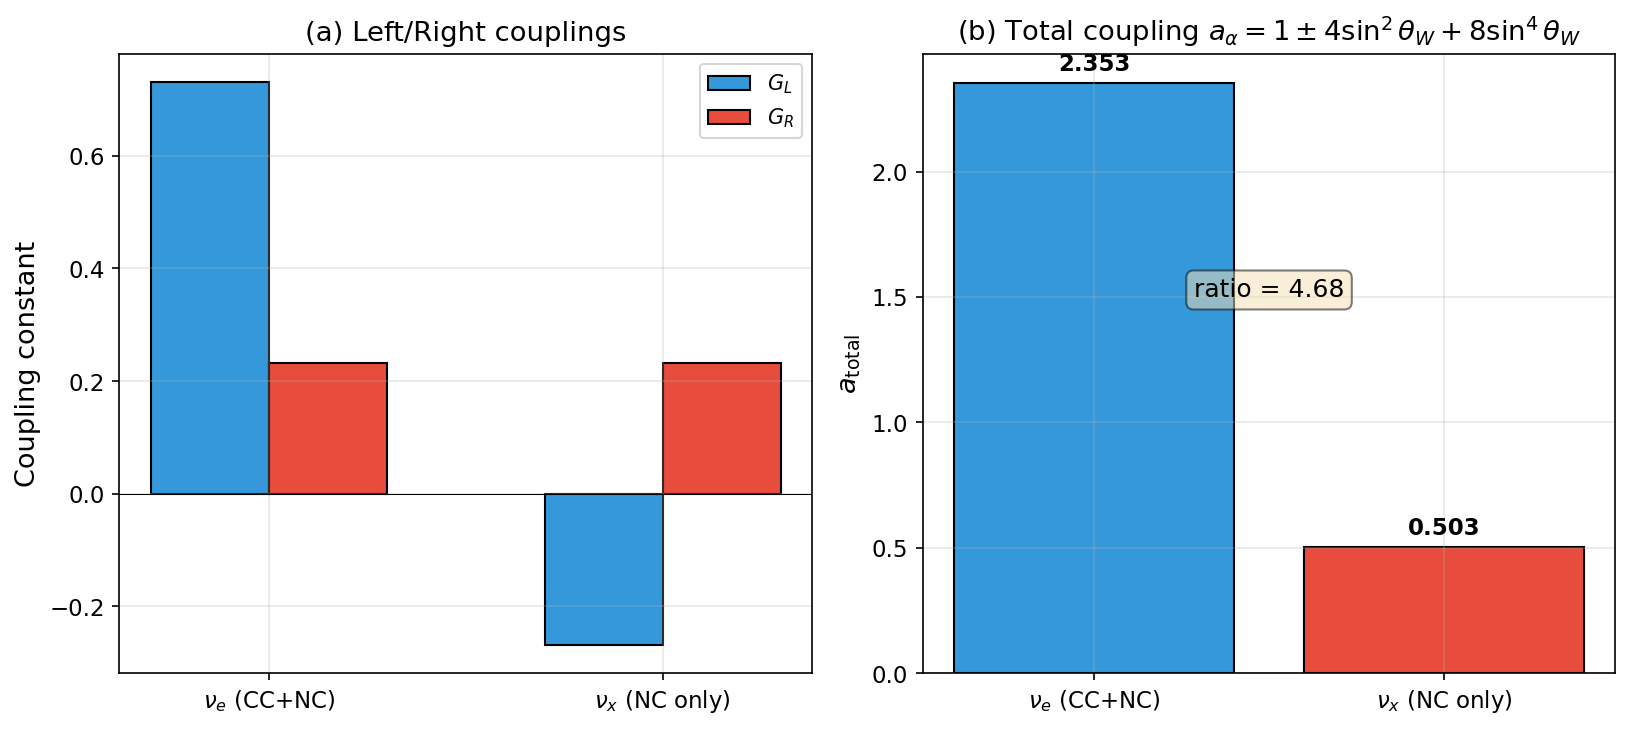
\includegraphics[width=\textwidth]{fig_ped08_coupling_constants.png}
\caption{Standard Model weak couplings for $\nu$--$e$ interactions.  (a)~Left- and right-handed couplings $\GL$, $\GR$ for $\nu_e$ (CC+NC) and $\nu_x$ (NC only); note $\GL^{\nu_x} < 0$.  (b)~Total coupling coefficients $a_\alpha$: the ratio $a_e/a_x \approx 4.68$ drives flavour-dependent spectral distortion during incomplete decoupling.}\label{fig:couplings}
\end{figure}

\subsection{The Reduced Collision Integral}

After angular integration, the collision integral for each neutrino momentum node $y_1$ takes the form
\begin{equation}
\bx{C_{\rm scat}[f](y_1) = \frac{\GF^2\,T^5}{4\pi^3}\int_0^\infty \dd y_2\int_0^\infty \dd y_3\;\Theta(y_4)\;|\mathcal{M}|^2(y_1,y_2,y_3,y_4)\;\mathcal{S}(f_1,f_2,f_3,f_4)\,,}\label{eq:C_scat}
\end{equation}
where $\Theta(y_4)$ enforces 4-momentum conservation $y_4 = y_1 + y_2 - y_3 > 0$, and $\mathcal{S}$ is the statistical factor.  With dimensionless $y_i$ and the dimensionless reduced kernel convention used here, the prefactor scales as $\GF^2T^5$: in natural units $C_{\rm scat}$ has dimensions of a rate, while $C_{\rm scat}/H$ is dimensionless in an e-fold evolution equation.

The historical spectral surface evaluated a reduced double integral on fixed
momentum grids and interpolated $f_\nu$ between nodes.  That implementation is
not current runtime authority.  The Rust F09B slice instead integrates only the
thermal energy moment described below; it does not yet evolve a spectral
distribution.
\subsection{Properties of the Collision Integral}

The collision terms satisfy the following exact reaction-level properties:

\begin{enumerate}
\item \textbf{Detailed balance}: $C[f_{\rm eq}] = 0$ when all species are at the same temperature.  This is guaranteed by the statistical factor $\mathcal{S}$, which vanishes identically for equilibrium distributions.

\item \textbf{Elastic-scattering number conservation}: for $\nu+e^\pm\leftrightarrow\nu+e^\pm$, the neutrino number moment vanishes, $\int_0^\infty y^2 C_{\nu,\rm scat}[f](y)\,\dd y=0$.  Its neutrino energy moment, $\int y^3 C_{\nu,\rm scat}\,\dd y$, is generally nonzero when the neutrino and electromagnetic distributions differ.  The electron-sector energy moment has the opposite value, so it is the combined $\nu+e^\pm$ energy that is conserved.

\item \textbf{Pair-process conservation}: $e^+e^-\leftrightarrow\nu\bar\nu$ does not conserve neutrino plus antineutrino number separately, but it creates or destroys the pair symmetrically and therefore conserves neutrino lepton number $n_\nu-n_{\bar\nu}$.  Its neutrino-sector energy moment is likewise generally nonzero; the conserved quantity is the combined $\nu+\bar\nu+e^-+e^+$ energy.
\end{enumerate}

Thus the neutrino-sector energy-transfer rate can be nonzero during transients (when $T_\gamma \neq T_\nu$) without violating total energy conservation.

\subsection{Current Rust F09B Thermal-Moment Slice}

The crate-private F09B source evaluates the invariant two-body phase space in
plasma-frame incoming coordinates and constructs the final state in the
centre-of-momentum frame.  It retains the vacuum electron mass, zero-chemical-
potential Fermi--Dirac occupations, Pauli blocking, and the tree-level
Hannestad--Madsen coupling convention.  The endpoint rule uses six-point
Gauss--Laguerre quadrature for each incoming radial momentum, four-point
Gauss--Legendre quadrature for the incoming and final polar angles, and eight
midpoint azimuths.  No fitted suppression factor, lookup table, or calibrated
$\Neff$ target enters.

An independently written NumPy/SciPy plasma-frame/CM integral reproduces every
production elastic and pair component at $T_\gamma=1.2\,\mathrm{MeV}$ and
$T_\nu=1.0\,\mathrm{MeV}$.  The production totals are $1.0473763830$ and
$0.2201082055$ for the electron and heavy flavours.  Raising the independent rule through
$(N_r,N_\mu,N_\phi)=(8,8,12),(12,10,16),(16,12,20),(24,16,24)$ changes the
electron- and heavy-flavour totals toward $1.0471753248$ and $0.2200659307$,
respectively, in units of $G_F^2$ factored out.  Thus the fixed endpoint rule carries a measured relative quadrature
remainder of about $1.9\times10^{-4}$ at this anchor; it is not continuum
truth.  A structurally different direct Hannestad--Madsen support/root
construction approaches the same finite-mass FD totals to about $0.3\%$ at
order 32 and recovers the analytic massless Maxwell--Boltzmann limit to about
$0.38\%$.

The four-point polar reduction is separately checked against the former
six-point rule at six temperature pairs from $10/9.99$ down to
$0.05/0.04\,\mathrm{MeV}$ and both flavour couplings; every total differs by
less than $2\times10^{-5}$ relatively.  A three-point rule was rejected
because its independent envelope errors reached $4.69\times10^{-5}$ and
$7.63\times10^{-5}$.  The accepted reduction changes the independent thermal
$\Neff$ anchor by about $9.1\times10^{-9}$ while reducing the measured Rust
BDF and Rodas5P cold-endpoint walls by factors $2.28$ and $2.16$ in the
most recent like-for-like runs.  This is a repeated-run prerequisite, not a
spectral-collision result or runtime promotion.

The executable checks also cover the exact common-temperature null,
temperature-ordering sign, nonnegative thermal entropy production, event-level
energy conservation, elastic neutrino-number and pair lepton-number topology,
one-electron-pair plus two-heavy-pair multiplicity, low-temperature electron
suppression, and the equal-and-opposite FLRW first law.  A separate adaptive-
EOS SciPy endpoint with DOP853 and Radau agrees before comparison with the Rust
BDF and Rodas5P endpoints.

This evidence validates only the isotropic thermal $\ell=0$ moment inside its
declared tree-level model.  Collision thermal masses, radiative collision
corrections, neutrino--neutrino reactions, spectral distortions, lepton
asymmetry, oscillations, QKE, precision $\Neff$/abundances, and public runtime
authority remain outside the claim.

\subsection{Current Rust F10B2 Resolution-Selected Spectral Substrate}

F10B1 first reused the same finite-mass HM support density to construct a collision
action at every node of the comoving $q=ap$ grid.  One occupation vector
represents the zero-lepton-asymmetry $\nu_e+\bar\nu_e$ pair and a second the
degenerate heavy pair; the FLRW energy readout applies the latter to both muon
and tau flavours.  No relaxation-time calibration enters.  The discrete
elastic event flux is antisymmetrised between incoming and outgoing neutrino
nodes, so its quadrature number moment vanishes by construction.  The pair
event flux is symmetrised between neutrino and antineutrino nodes, so their
number changes are equal and the lepton-number difference is conserved.  Both
identities pass at a $5\times10^{-12}$ relative roundoff ceiling even for
unequal test occupations.

The Pauli gain/loss algebra supplies the occupation Jacobian analytically.  An
exact common-temperature FD reference branch enforces the analytic detailed-
balance null, while non-equilibrium values and derivatives retain the direct
event evaluation.  The action's energy moment is transferred with the opposite
sign to the electromagnetic bath.  Focused finite differences check the
folded action and FLRW Jacobians, and the combined first law closes to
$3\times10^{-15}$ relatively.

F10B2 addresses the numerical-coordinate and resolution blockers without
changing this action.  A direct-occupation 12-node Rodas5P run failed raw when
a far-tail occupation approached floating-point zero.  The evolved variable
is therefore now the exact logit $u=\ln[f/(1-f)]$; a stable logistic map and
chain-rule Jacobian preserve $0<f<1$, while unrepresentable underflow still
fails rather than being clipped.  Event order four/three is rejected.  At
$T_\gamma/T_{\rm cm}=1.2/1.0$, the retained 16-node/event-six/four energy
moments are $0.99078$ and $0.99087$ of the independent F09B thermal totals for
electron and heavy flavours.  The high-order $32/32/24$ component check gives
$1.00162$ and $1.00170$.

With the retained rule, the private cold-event regressions are
\begin{align*}
(N,t,\Neff)_{\rm BDF}
  &= (7.9367312298,52681.0360\,\mathrm{s},3.0330775769),\\
(N,t,\Neff)_{\rm Rodas5P}
  &= (7.9367453070,52681.5412\,\mathrm{s},3.0329326538).
\end{align*}
A same-code BDF ladder at 12, 16, and 20 nodes gives
$\Neff=3.0326021077$, $3.0330775769$, and $3.0331966346$; the final change is
$1.19\times10^{-4}$.  The grid-20 Rodas leg and a structurally independent
full spectral solve were not run.  A five-point explicit-$N$ step ladder bounds
the direct-support sensitivity in the executable tests.  Consequently this is
a resolution-selected conservation/coupling substrate, not a precision
distortion or $\Neff$ prediction.  Neutrino--neutrino reactions, collision
thermal/radiative corrections, lepton asymmetry, oscillations, QKE, and public
runtime authority remain outside the claim.

\subsection{Rust F10C0 Component and F10C1 Radial Selection}

F10C0 adds one deliberately restricted classical neutrino--neutrino channel
to the isotropic Rust action: massless diagonal
$\nu_\alpha+\nu_\alpha\leftrightarrow\nu_\alpha+\nu_\alpha$ and the identical
antineutrino reaction, with zero lepton asymmetry.  It acts separately on the
electron and degenerate-heavy occupation blocks; it does not couple flavours
or neutrinos to antineutrinos.  This completes row 1 and implements the
same-flavour-identical subset of row 3 in the nine-row folded zero-lepton
catalogue motivated by the standard
decoupling collision treatments
\cite{HannestadMadsen1995,Dolgov1997,Froustey2020}, not an implementation of
the complete catalogue.

In the natural-unit convention of the Rust kernel, define
$K_s=(p_1\!\cdot p_2)(p_3\!\cdot p_4)$.  The directed physical event carries
$32\,\GF^2K_s$.  The global four-leg weak form includes the elastic
time-orientation factor $\eta=1/2$ and therefore carries
$16\,\GF^2K_s$; the four tagged-leg appearances recover the corrected
$64\,\GF^2K_s$ target-row coefficient.  The implementation integrates each
event in centre-of-momentum coordinates.  Both off-grid outgoing logits are
evaluated with the same nonnegative linear basis used to deposit the two
outgoing legs, and an event is omitted as a whole if either outgoing leg lies
outside the finite radial domain.  This shared partition-of-unity basis
preserves the discrete number and energy moments event by event, while the
stable Pauli gain--loss form supplies nonnegative entropy production and an
analytic Jacobian with respect to the evolved logits.

Within this restricted channel, the component claims are
\textbf{VALIDATED}: the executable checks recover the analytic tagged
massless Maxwell--Boltzmann loss with the corrected coefficient, give the
common affine Fermi--Dirac null, preserve nonthermal number and energy, recover
the $\GF^2T^5$ scaling, and compare the analytic logit Jacobian with a
five-point stencil.  A production-versus-tagged nonthermal weak-action oracle
on compact quadratic radial rules reaches a relative residual of
$2.07348\%$ at radial order 64.  At the historical F10C0 boundary this did
\emph{not} validate its endpoint grid: the 16-node Gauss--Laguerre linear
radial representation was approximately $7.54\%$ below the high-resolution
tagged weak-action oracle.

F10C1 keeps the same nonnegative linear interpolation and deposition algebra
but replaces that historical grid with a fixed positive 48-node rule,
$y=-3\ln(1-t)$ for Gauss--Legendre $t\in(0,1)$.  There is no user-imposed
integration cutoff, although the finite extreme nodes still bound the
interpolation support and whole outgoing events outside it remain rejected.
The direct weak-action residuals at N32, N40, N48, and N64 are
$1.873525\%$, $1.227393\%$, $0.852441\%$, and $0.489704\%$.  This scalar
ladder is necessary but not sufficient.  Selection is controlled by five
smooth nonthermal profiles integrated on both compact and exponential N128
auxiliary rules.  Their worst state-basis residual is
$1.9771546\%<2.1\%$; the exact auxiliary references agree within
$1.93\times10^{-8}$ relatively, while number and energy close below
$1.8\times10^{-14}$.  Composite N32 and exponential N32/N40 are rejected by
the auxiliary or electron-anchor gates despite favourable lower-dimensional
comparisons.  Thus the N48 representation is \textbf{VALIDATED} only for this
declared profile envelope, not for arbitrary distributions, continuum truth,
or precision decoupling.

The distinct-heavy part of row 3 remains absent, as do all channels in rows 2
and 4--9---including cross-flavour elastic, $\nu\bar{\nu}$ elastic, and
pair-conversion structures.  These catalogue parts remain \textbf{SPECIFIED}.
QKE remains
\textbf{FORBIDDEN} on this programme.  The radial-grid choice is no longer the
active task.  A prepared self-event-geometry candidate reduced the matched N48
cold wall from $2181.07$ to $1980.52\,\mathrm{s}$ ($9.195\%$), below the
programme's approximately $10\%$ partial-blocker threshold, while maximum RSS
rose by $3.277\%$; its 112 Rust lines and cache-only test were therefore
removed.  The remaining cold-endpoint cost must be attacked at its measured
dominant consumer without a new readiness or table surface before row 3 is
completed and the seven wholly absent rows are added from the frozen
catalogue.

On the retained no-cache tree, both BDF and Rodas5P then reproduced their
pre-cache endpoint states bitwise.  The matched run took
$2191.66\,\mathrm{s}$ with maximum RSS $50{,}440\,\mathrm{KB}$, corresponding
to a $0.486\%$ wall increase and a $1.137\%$ RSS decrease relative to the
initial no-cache record.  The retained electron values-only allocation
cleanup is therefore an arithmetic-neutral simplification with no claimed
endpoint acceleration.  The approximately 36-minute cold wall, the partial
row 3, the seven absent rows, and a structurally independent full-spectral
FLRW comparison all remain open F10 gates.

The current owner-authorized programme ends after those F10 gates close and a
collision-coupled isotropic FLRW handoff is validated.  LRS and non-LRS
Type-I/Bianchi extensions are owner-paused; QKE and public-production claims
remain \textbf{FORBIDDEN}.  None of those later structures is opened by the
component or radial evidence reported here.

%======================================================================


\section{Pair Annihilation and Creation}\label{sec:pair}
%======================================================================

The pair process $\nu_\alpha + \bar\nu_\alpha \leftrightarrow e^+ + e^-$ has a different matrix element structure from elastic scattering.  At tree level in the Standard Model:
\begin{equation}
|\mathcal{M}|^2_{\rm pair} \propto (\GL^2 + \GR^2)\bigl[(y_1 y_4)^2 + (y_2 y_3)^2\bigr] + (\GL^2 - \GR^2)\bigl[(y_1 y_3)^2 + (y_2 y_4)^2\bigr]\,,
\end{equation}
where the crossing symmetry exchanges $(y_2 \leftrightarrow y_4)$ compared to scattering, reflecting the different Mandelstam-variable assignments.

The pair collision integral is
\begin{equation}
C_{\rm pair}[f_\nu, f_{\bar\nu}](y_1) = \frac{\GF^2\,T^5}{4\pi^3}\int \dd y_2\,\dd y_3\;\Theta(y_4)\;|\mathcal{M}|^2_{\rm pair}\;\mathcal{S}_{\rm pair}\,,
\end{equation}
where the statistical factor now involves the anti-neutrino:
\begin{equation}
\mathcal{S}_{\rm pair} = f_{e^+}(y_3)\,f_{e^-}(y_4)\,(1-f_\nu)(1-f_{\bar\nu}) - f_\nu\,f_{\bar\nu}\,(1-f_{e^+})(1-f_{e^-})\,.
\end{equation}

The total collision integral for species $\alpha$ is the sum:
\begin{equation}
C_\alpha[f] = C_{\rm scat}^\alpha + C_{\rm pair}^\alpha\,.
\end{equation}

%======================================================================


\section{Relaxation-Time Approximation}\label{sec:rta}
%======================================================================

\subsection{Motivation}

The full 2D integral \eqref{eq:C_scat} is computationally expensive ($\order(N_q^3)$ per timestep).  Historically, the PSTF hierarchy used a calibrated relaxation-time approximation (RTA) as an inexpensive damping surrogate when only the multipole moments $\Psi_0$ and $\Psi_2$ were tracked.

\paragraph{Current status.} This RTA, including the fitted value $C_{\rm rate}=210$ and the electron-suppression profile below, is \textbf{DEPRECATED}.  It is retained only to document the historical calibration; it is neither the F09 collision-source authority nor evidence for a current Rust endpoint or precision-$\Neff$ result.

\subsection{The RTA Model}

The RTA replaces the full collision integral with a linear damping term:
\begin{equation}
\bx{C_\ell[\Psi_\ell](q) = -\kappa_\ell\,\frac{\Gamma_s}{H}\,\Psi_\ell(q)\,,}\label{eq:rta}
\end{equation}
where $\Gamma_s$ is the scattering rate and $\kappa_\ell$ is a multipole-dependent damping coefficient:
\begin{align}
\kappa_0 &= 1\,,\\
\kappa_2 &= \frac{5}{3}\,.
\end{align}

The historical quadrupole damping coefficient $\kappa_2 = 5/3$ was chosen to model faster isotropisation of higher multipoles, and the overall calibration targeted $\Neff\approx3.044$.  That target-matching construction is not an independent derivation or validation of the collision physics.

The scattering rate per e-fold is
\begin{equation}
\frac{\Gamma_s}{H} = \frac{C_{\rm rate}}{\pi^5}\,\GF^2\,a_s\,F(m_e/T_\gamma)\,T_\gamma^4\,T_\nu\,\frac{1}{H}\,,
\end{equation}
where the deprecated value $C_{\rm rate} = 210$ is a historical calibration constant, $a_s$ is the species-dependent coupling ($a_e$ or $a_x$), and $F(m_e/T_\gamma)$ is a fitted electron mass suppression factor:
\begin{equation}
F(x) = \frac{1}{1 + e^{2.5(x - 2.3)}}\,,
\end{equation}
which smoothly turns off the collision rate when $T_\gamma \lesssim m_e/2.3 \approx 0.22\;\mathrm{MeV}$ and $e^\pm$ pairs are Boltzmann-suppressed.

\subsection{Limitations of the RTA}

The RTA has a fundamental limitation: \textbf{it has no source term}.  When $\Psi_\ell = 0$, $C_\ell = 0$ regardless of whether $T_\gamma \neq T_\nu$.  This means the RTA \emph{cannot generate} the spectral distortion from incomplete decoupling; it can only \emph{damp} existing perturbations toward equilibrium.

Any current source-bearing treatment must instead specify and validate its energy-transfer or phase-space collision operator, including its approximation limits and conservation checks.  The historical RTA cannot serve as that authority.

%======================================================================


\section{Incomplete Decoupling and Neff}\label{sec:incomplete_decoupling}
%======================================================================

\subsection{The Physical Problem}

In the standard FLRW picture, neutrino decoupling at $T \sim 1$--$3\;\mathrm{MeV}$ is \emph{incomplete}: during $e^+e^-$ annihilation ($T \lesssim m_e$), residual weak interactions transfer part of the electromagnetic entropy to neutrinos.  This raises the total neutrino energy density above the instantaneous-decoupling value, giving the Standard-Model benchmark $\Neff = 3.044$ instead of $3.000$ \cite{Mangano2005, deSalas2016, Froustey2020, Bennett2020}.  Physically, the correction combines an overall reheating effect with a momentum-dependent spectral distortion, since high-energy neutrinos continue to scatter longer than low-energy ones.

For the present report, however, the key scope statement is different from the textbook one: \emph{the historical exact-characteristic Type~I figures do not rely on a full quantum-kinetic or fully collision-coupled anisotropic Boltzmann treatment of incomplete decoupling}.  Instead, the reference figures rest on a collisionless characteristic-transport core, while incomplete-decoupling effects enter through a tiered approximation hierarchy.  The repository retains historical tier~2 and no-Teff tier~3 JAX surfaces, but these do not amount to a full anisotropic collision-coupled scattering closure.

\paragraph{Current backend authority.} Rust AOT is the active implementation and repeated-run target.  SciPy/BDF remains the temporary number-of-record until the Rust endpoint authority gate passes.  JAX is frozen as a historical component-level parity/automatic-differentiation/Jacobian oracle; it is not an active forward-development, endpoint, runtime-promotion, or production authority.

\paragraph{Current F09B Rust slice.} A crate-private Rust endpoint now evolves
three thermal temperatures with a finite-vacuum-electron-mass, FD/Pauli,
tree-level electron/positron energy-transfer moment.  The same source is
consumed by the corrected weak leg and selected 31-reaction network.  At the
QED-off FLRW anchor $T_\gamma=0.005\,\mathrm{MeV}$, an independently written
adaptive-EOS/CM-integral solve gives
$N=7.93669848685$, $T_{\nu_e}=0.00358318527739\,\mathrm{MeV}$,
$T_{\nu_x}=0.00357679030100\,\mathrm{MeV}$, and the thermal readout
$N_{\rm eff}=3.03409326175$.  DOP853 and Radau agree to
$5.4\times10^{-12}$ in $N$ and below $3.0\times10^{-13}\,\mathrm{MeV}$ in
the neutrino temperatures before the Rust comparison.  This number is a
regression result for the declared thermal tree-level model, not a precision
Standard-Model prediction: spectral transport, neutrino--neutrino reactions,
oscillations, collision QED corrections, and an independently validated
QED-on nuclear endpoint are absent.

\subsection{Tiered Treatment in RABBIT}

The safest description of the current implementation is therefore not ``full treatment'' but \emph{tiered treatment of incomplete decoupling}.  The code contains several levels of thermodynamic and collision-aware sophistication, and the current repository surface is broader than the historical exact-characteristic figures alone.  Table~\ref{tab:decoupling_scope} summarises the intended interpretation.

\begin{table}[t]
\centering
\small
\caption{Historical scope of the incomplete-decoupling hierarchy. ``Used for the quoted report figures?'' refers specifically to the historical exact-characteristic reference results discussed in this report; implementation inventory does not imply current backend authority.}\label{tab:decoupling_scope}
\begin{tabularx}{\textwidth}{p{1.35cm}X>{\centering\arraybackslash}p{1.35cm}>{\centering\arraybackslash}p{1.8cm}p{3.0cm}}
\toprule
Level & Description & Impl.? & Used in quoted figures? & Claim scope \\
\midrule
Tier~1 & Parametric / effective thermodynamic closure; instantaneous-decoupling baseline plus production helper thermodynamics. & Yes & Yes & Historical reference baseline; the retained JAX implementation is a frozen component oracle only. \\
Tier~2 & Coupled three-temperature incomplete-decoupling extension with momentum-averaged $\nu$--$e$ energy transfer and QED-plasma feedback. & Yes & No & Historical JAX component surface; not the F09 collision or endpoint authority. \\
Tier~3 & No-Teff three-temperature weak-budget ladder with CL0--CL3 support. & Yes & No & Historical JAX component surface; not a full anisotropic collision-coupled Boltzmann solver. \\
Tier~4 & Tier~3 plus flavour oscillations and the full SM target. & Deferred & No & Explicitly out of scope. \\
\bottomrule
\end{tabularx}
\normalsize
\end{table}

This hierarchy should be read with three distinct labels in mind.
\begin{enumerate}
\item \textbf{Reference-result claim}: the historical exact-characteristic figures and CL2 profile constraint quoted elsewhere in this report.
\item \textbf{Frozen component-oracle claim}: the retained JAX tier~1--3 surfaces may support local parity, AD, and Jacobian checks only; they do not establish forward-solver or runtime authority.  SciPy/BDF is the temporary number-of-record, not a Rust promotion result.
\item \textbf{Out-of-scope claim}: full QKE, full anisotropic collision integrals, species-resolved end-to-end scatter on exact rays, and complete $\nu$--$\nu$ plus $\nu$--$e$ angular closure.
\end{enumerate}

With that distinction in place, the phrase ``incomplete decoupling'' in the remainder of this document should always be read as a \emph{controlled approximation hierarchy} rather than as a claim that the full anisotropic scattering problem has already been solved end to end.

\subsection{Entropy Conservation with Collision Source Term}

The fundamental thermodynamic equation governing photon-temperature evolution is entropy conservation of the $\gamma+e^\pm$ plasma, augmented by a source term describing neutrino--electron energy exchange.  Let $\mathcal S = s_{\rm plasma}a^3$ be the comoving electromagnetic entropy, with $s_{\rm plasma}=(\rho_{\rm plasma}+p_{\rm plasma})/T_\gamma$.  Then
\begin{equation}
\frac{\dd}{\dd t}(s_{\rm plasma}a^3) = -\frac{1}{T_\gamma}\,\frac{\dd Q_{\nu\to{\rm plasma}}}{\dd t}\,a^3\,,\label{eq:entropy_full}
\end{equation}
where $\dd Q_{\nu\to{\rm plasma}}/\dd t$ is positive when neutrinos lose energy to the plasma.

Writing $s_{\rm plasma}=S(T_\gamma)T_\gamma^3$ and differentiating with respect to $N=\ln a$ gives
\begin{equation}
\frac{\dd}{\dd N}\bigl[S(T_\gamma)T_\gamma^3\bigr] = \bigl(3S+T_\gamma S'\bigr)T_\gamma^2\frac{\dd T_\gamma}{\dd N}+3ST_\gamma^3\,.
\end{equation}
Solving for the temperature derivative yields the thermodynamic master equation
\begin{equation}
\bx{\frac{\dd T_\gamma}{\dd N} = -\frac{T_\gamma}{1 + T_\gamma S'/(3S)}\left(1 - \frac{\dd Q}{T_\gamma^4\,(\dd\rho/\dd T)_\gamma}\right)\,.}\label{eq:dTgamma_dN}
\end{equation}
In the historical hierarchy, Tier~1 supplied the source term through an effective closure, while Tier~2 used a partially live collision-aware module.  This describes the approximation structure only; it does not promote either historical JAX surface to current collision or endpoint authority.

At Tier~2+, the energy-transfer functional is obtained from the collision operator:
\begin{equation}
\frac{\dd Q_{\nu\to\rm plasma}}{\dd t} = -\sum_\alpha \int \frac{\dd^3\mathbf p}{(2\pi)^3}\,E\,C_\alpha[f_\alpha] \, ,
\end{equation}
and, using the momentum variable $y=p/T_\nu$,
\begin{equation}
\frac{\dd Q}{\dd N} = -\frac{T_\nu^4}{2\pi^2 H}\sum_\alpha\int_0^\infty \dd y\; y^3 C_\alpha[f_\alpha](y)\,.
\end{equation}
These expressions are kept because they are the natural bridge between the thermodynamic equation and the Tier~2 extension, even though the fully anisotropic evaluation of $C_\alpha$ remains outside current endpoint authority.

\subsection{Momentum-Dependent Decoupling}

\begin{figure}[t]
\centering
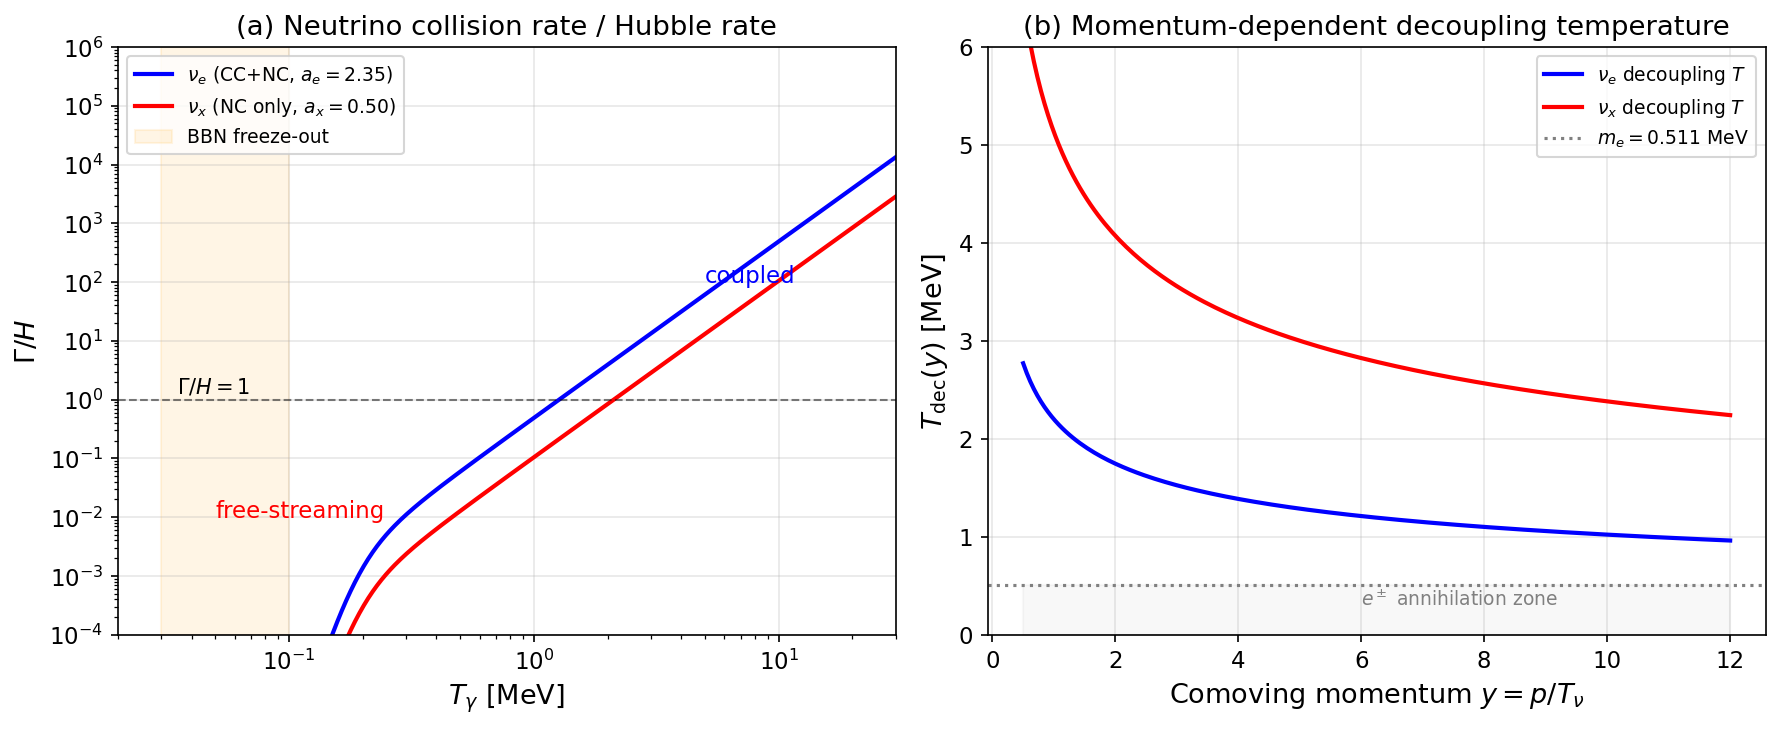
\includegraphics[width=\textwidth]{fig_ped02_collision_rate_profile.png}
\caption{Neutrino collision rates.  (a)~$\Gamma/H$ vs photon temperature for $\nu_e$ (blue, CC+NC coupling) and $\nu_x$ (red, NC only).  The decoupling condition $\Gamma/H = 1$ is reached at $T \approx 1.5\;\mathrm{MeV}$ for $\nu_e$ and $T \approx 3.5\;\mathrm{MeV}$ for $\nu_x$.  (b)~Momentum-dependent decoupling temperature $T_{\rm dec}(y) \propto y^{-1/3}$: high-momentum neutrinos decouple later and receive more heating from $e^+e^-$ annihilation.}\label{fig:collision_rate}
\end{figure}

The collision rate for a neutrino with dimensionless momentum label $y$ scales approximately as $\Gamma(y) \propto G_F^2T^5 y$, so high-momentum neutrinos remain coupled longer than low-momentum neutrinos.  A useful estimate of the decoupling temperature is
\begin{equation}
T_{\rm dec}(y) \approx T_{{\rm dec},0}\left(\frac{y}{3.15}\right)^{-1/3},
\end{equation}
with $T_{{\rm dec},0}\approx 1.5\;\mathrm{MeV}$ for $\nu_e$ near the thermal peak.  The consequence is a momentum-dependent reheating pattern: low-$y$ modes decouple early and miss most of the $e^+e^-$ entropy release, while high-$y$ modes remain coupled longer and are heated more strongly.

To display this effect without confusing the dimensionless transport label $y=p/T_\nu$ with a physical temperature, it is safer to define a \emph{diagnostic effective temperature at fixed physical momentum} $p$ by
\begin{equation}
T_{\rm eff}(p) \equiv \frac{p}{\ln\!\bigl(1/f(p)-1\bigr)}\,.
\end{equation}
For a perfect Fermi--Dirac spectrum, $T_{\rm eff}(p)=T_\nu$ is independent of $p$; after incomplete decoupling, $T_{\rm eff}(p)$ rises at high $p$, signalling spectral hardening.  In the present report this quantity is used only as a diagnostic descriptor of the Tier~2 extension, not as a separate production dynamical variable.

\begin{figure}[t]
\centering
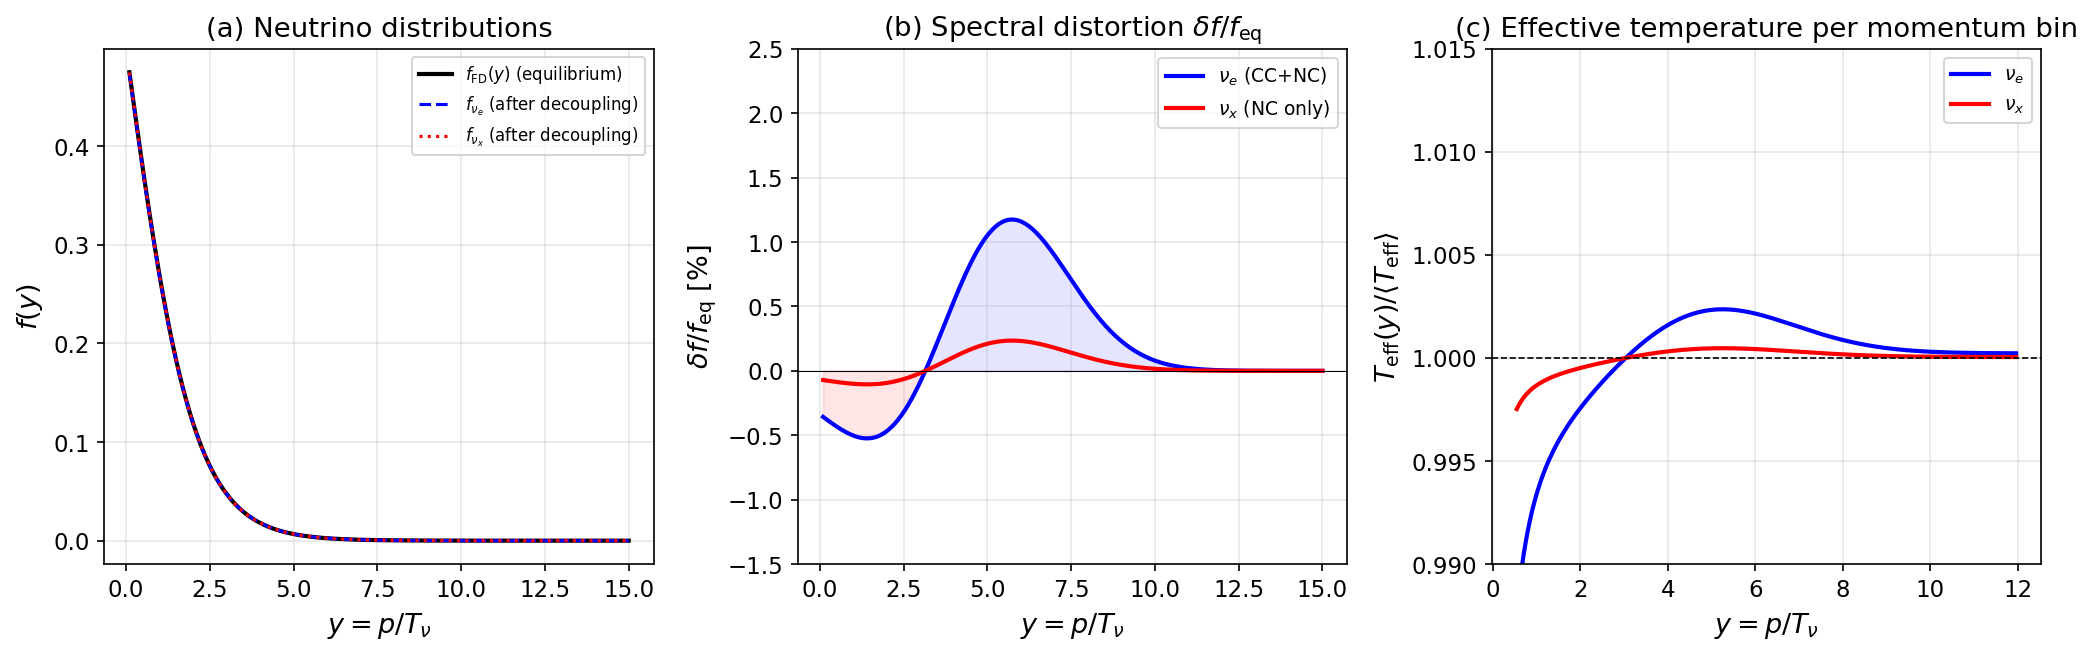
\includegraphics[width=\textwidth]{fig_ped03_spectral_distortion.png}
\caption{Neutrino spectral distortion from incomplete decoupling (schematic, based on Mangano et~al.\ 2005).  (a)~Distribution functions: the distorted $f_{\nu_e}$ (dashed) shows excess at high $y$ relative to equilibrium (solid).  (b)~Fractional distortion $\delta f/f_{\rm eq}$: positive at $y > 3$ and negative at $y < 3$.  (c)~A diagnostic effective-temperature representation showing the corresponding hardening trend.}\label{fig:spectral_dist}
\end{figure}

\subsection{Connection to Anisotropic BBN}

In anisotropic Bianchi cosmologies, incomplete decoupling acquires two distinct layers of relevance.  First, even at the level of the production baseline, the decoupling condition $\Gamma/H$ is altered by the shear-enhanced Hubble rate
\begin{equation}
H=H_{\rm FLRW}/\sqrt{1-\Sig^2}
\end{equation}
so decoupling occurs earlier when $\Sig>0$.  This is the leading anisotropic effect relevant for the present BBN forward model.

Second, once one goes beyond the production baseline, the neutrino distribution ceases to be both isotropic and exactly thermal.  A fully faithful treatment would then require species-, momentum-, and angle-resolved scattering on top of exact ray transport.  That problem is \emph{not} solved here end to end.  The historical Tier~2 modules remain available for bounded component checks, without establishing a complete anisotropic scattering closure or a validated BBN correction.

The report retains Tier~2 for provenance and bounded component comparison.  It is not a production headline, an active runtime path, or validation of the deferred anisotropic collision-coupled problem.

\subsection{\texorpdfstring{$N_{\rm eff}$}{Neff} in the tiered hierarchy}

The effective number of neutrino species is defined operationally by
\begin{equation}
\Neff \equiv \frac{8}{7}\left(\frac{11}{4}\right)^{4/3}\frac{\rho_\nu}{\rho_\gamma}\,.
\end{equation}
What changes across tiers is not this definition but the approximation used for $\rho_\nu$.

At the instantaneous-decoupling level one has
\begin{equation}
\rho_\nu^{\rm inst} = N_\nu\,\frac{7\pi^2}{120}T_\nu^4,
\qquad T_\nu/T_\gamma=(4/11)^{1/3},
\end{equation}
which gives $\Neff=3.000$ before any reheating correction is added.  A purely parametric helper can then impose the Standard-Model benchmark $\Neff=3.044$ by hand.

In the intended historical Tier~2 formulation, the neutrino energy density would instead be computed from the evolved non-equilibrium spectrum,
\begin{equation}
\rho_\nu = \sum_\alpha \frac{T_\nu^4}{2\pi^2}\int_0^\infty \dd y\; y^3 f_\alpha(y)
\end{equation}
but this expression alone does not validate a numerical $\Neff$ prediction.  Missing $\nu$--$\nu$ scattering, flavour oscillations, and full collision closure prevent a Standard-Model precision claim.  The frozen no-Teff tier~3 JAX surface likewise remains a component oracle rather than a full species- and angle-resolved collision solver.

\subsection{The Full Boltzmann Equation for Incomplete Decoupling}

At Tier~2, the evolution equation for each neutrino species $\alpha$ in the thermal momentum variable $y \equiv p/T_\nu$ is
\begin{equation}
\bx{\frac{\partial f_\alpha(y)}{\partial N} = -\frac{\dd\ln y}{\dd N}\,y\,\frac{\partial f_\alpha}{\partial y} + \frac{C_\alpha[f_\alpha, f_e](y)}{H}\,,}\label{eq:boltzmann_tier2}
\end{equation}
where $C_\alpha$ includes both scattering and pair processes.  In the FLRW limit, there is no angular dependence ($\dd\mu/\dd N = 0$), and the problem reduces to solving $N_q$ coupled ODEs per neutrino species for the distribution values $f_\alpha(y_i)$ at each momentum node.

\paragraph{Current F10A collisionless substrate.} The first Rust spectral
slice fixes the comoving coordinate $q=ap$, with $a=1$ at the initial state,
instead of using a moving physical-momentum grid.  For massless collisionless
neutrinos the Liouville equation is therefore represented exactly as
\begin{equation}
\left.\frac{\dd f(q_i)}{\dd N}\right|_{C=0}=0,
\qquad
n_{\nu\bar\nu}=\frac{e^{-3N}}{\pi^2}\sum_iw_iq_i^2f_i,
\qquad
\rho_{\nu\bar\nu}=\frac{e^{-4N}}{\pi^2}\sum_iw_iq_i^3f_i .
\end{equation}
The distribution energy density enters the Friedmann rate and hence an
evolved cosmic-time state in the photon-temperature endpoint; it is not a
detached moment check.  With 24 Gauss--Laguerre nodes, Rust BDF/Rodas5P reach
$N=7.93804264043/7.93804264041$ and elapsed time
$52796.0351546/52796.0351521\,\mathrm{s}$ at
$T_\gamma=0.005\,\mathrm{MeV}$.  A separately written adaptive-EOS continuum-
FD SciPy solve gives $N=7.93804264044$ and
$52796.0351521\,\mathrm{s}$; DOP853 and Radau agree before the Rust comparison.
Orders 12, 24, and 36 converge to the analytic FD number and energy moments,
and arbitrary occupations preserve $n_\nu a^3$ and $\rho_\nu a^4$.

At the F10A boundary this closed only collisionless isotropic classical
redshifting and the energy-grid state convention; it supplied no collision or
distortion claim.

\paragraph{Current F10B2 electron action.} F10B1 first evaluated the
finite-mass HM electron/positron event action on the same grid for separate
electron and degenerate-heavy flavour-pair occupations.  Conservative
antisymmetric elastic fluxes preserve the quadrature number moment, symmetric
pair fluxes preserve neutrino-minus-antineutrino number, and the analytic
Pauli response supplies the occupation Jacobian.  The collision energy moment
is debited equal-and-opposite from the electromagnetic bath.  The exact common
FD reference is an analytic action null; five-point action/FLRW derivatives and
the combined first law pass.  F10B2 stores the evolved occupations as exact
logits, after a direct-occupation 12-node Rodas run failed raw in the
floating-point tail.  Stable logistic reconstruction and the chain-rule
Jacobian preserve strict open occupations without clipping; unrepresentable
underflow still fails raw.

A separated momentum/event ladder rejects event order four/three and retains
16 momentum nodes with event order six/four.  Its electron/heavy thermal energy
moments are $0.99078/0.99087$ of the independent thermal anchors.  BDF and
Rodas5P reach
$(N,t,\Neff)=(7.9367312298,52681.0360\,\mathrm{s},3.0330775769)$ and
$(7.9367453070,52681.5412\,\mathrm{s},3.0329326538)$ at
$T_\gamma=0.005\,\mathrm{MeV}$.  A same-code grid-20 BDF refinement gives
$\Neff=3.0331966346$, while an explicit-$N$ step ladder bounds direct-support
sensitivity.  Grid-20 Rodas and an independent full spectral solve were not
run.  These remain test-only regression readouts: no precision distortion or
$\Neff$ claim, neutrino--neutrino collision, lepton asymmetry, flavour
coherence, anisotropy, QKE, or public runtime claim follows.

\paragraph{Historical F10C0 GL16 and current F10C1 N48 endpoint.} The FLRW
right-hand side consumes the restricted same-flavour
$\nu_\alpha\nu_\alpha\leftrightarrow\nu_\alpha\nu_\alpha$ action and the
identical antineutrino channel.  Because this elastic self-action conserves
its discrete neutrino energy moment event by event, it introduces no
electromagnetic energy-transfer source.  At the historical F10C0 boundary,
with the 16-node Gauss--Laguerre momentum grid, electron event order six/four,
and self-scattering angular order 12, the private cold-event regressions were
\begin{align*}
(N,t,\Neff)_{\rm BDF}
  &= (7.9367292791,52680.9384\,\mathrm{s},3.0331059589),\\
(N,t,\Neff)_{\rm Rodas5P}
  &= (7.9367451102,52681.5251\,\mathrm{s},3.0329371816).
\end{align*}
The selected linear action was approximately $7.54\%$ below the high-
resolution tagged oracle, so these values remain historical
\textbf{IMPLEMENTED} regressions rather than radial or precision authority.

F10C1 retains the same coefficient, Pauli algebra, and conservative linear
deposition but selects the positive exponential N48 rule
$y=-3\ln(1-t)$.  The initial no-cache N48 run gives
\begin{align*}
(N,t,\Neff)_{\rm BDF}
  &= (7.9367214190,52680.2048\,\mathrm{s},3.0333103242),\\
(N,t,\Neff)_{\rm Rodas5P}
  &= (7.9367373740,52680.8451\,\mathrm{s},3.0331291370).
\end{align*}
The direct N32--N64 ladder decreases from $1.873525\%$ to $0.489704\%$,
and two independent N128 auxiliary integrations bound five declared smooth
nonthermal profiles by $1.9771546\%<2.1\%$.  This is
\textbf{VALIDATED} only as a profile-bounded radial representation; it is not
arbitrary-distribution, continuum, complete-catalogue, precision-$\Neff$, or
independent full-spectral authority.

The initial matched no-cache endpoint took $2181.07\,\mathrm{s}$ with maximum
RSS $51020\,\mathrm{KB}$.  A prepared self-event-geometry candidate took
$1980.52\,\mathrm{s}$, only $9.195\%$ faster and below the programme's
approximately $10\%$ partial-blocker threshold, while RSS rose by $3.277\%$.
Its 112 Rust lines and cache-only test were removed; this negative result is
\textbf{DEPRECATED} evidence, not endpoint promotion.
The retained no-cache tree repeats both solver outputs bitwise in
$2191.66\,\mathrm{s}$ with maximum RSS $50440\,\mathrm{KB}$, respectively
$+0.486\%$ and $-1.137\%$ relative to the initial no-cache run.  The cold
wall is therefore unchanged.

Catalogue row 1 is complete and the same-flavour-identical subset of row 3
executes.  The distinct-heavy remainder of row 3 and every channel in rows 2
and 4--9 remain \textbf{SPECIFIED} but absent, so row 3 is partial and seven
rows are wholly absent.  Anisotropic collision closure, oscillations, QKE,
and public runtime authority do not follow; the measured N48 cold wall remains
the active task before catalogue expansion.  By owner decision the present
programme stops after this collision-coupled isotropic FLRW milestone is
completed and validated; Bianchi/LRS/non-LRS work requires a separate future
instruction.

When anisotropy is present, the full Boltzmann equation along a characteristic ray $j$ becomes
\begin{equation}
\bx{\frac{\partial f_j(y)}{\partial N} = -\left(\frac{\dd\ln y}{\dd N}\right)_{\!j}\,y\,\frac{\partial f_j}{\partial y} + \frac{C[f](y, \mu_j)}{H}\,,}\label{eq:boltzmann_char_coll}
\end{equation}
where $(\dd\ln y/\dd N)_j$ is the gravitational redshift along ray $j$ (determined by the anisotropic geometry), and $C[f](y, \mu_j)$ is the collision integral evaluated at the direction $\mu_j$ of ray $j$.

This equation poses a fundamental challenge: the collision integral $C[f](y, \mu_j)$ requires knowledge of $f$ at \emph{all} directions $\mu$ (through the angular integration in the matrix element), but each characteristic ray only carries information about its own direction $\mu_j$.  The current production report therefore treats the fully anisotropic collision-coupled problem as deferred full phase-space scope rather than as an active reduced bridge.

\subsection{The State Vector for Full Boltzmann}

In the full phase-space ray approach (Paper~II scope), the state per ray becomes $f_j(y_k)$ at $N_q$ momentum nodes, rather than the reduced characteristic variables.  The DOF comparison is:

\begin{center}
\begin{tabular}{lcc}
\toprule
Approach & State representation & Indicative size \\
\midrule
Characteristic reference (explicit) & $(I_j, J_j)$ + shared $S$ & $2N_\mu + 1 = 25$ transport DOF \\
Characteristic JAX compact & shared $S$ with analytic $I_j(S), J_j(S)$ & 13 total DOF (tier~1), 15 total DOF (tier~2) at $N_\mu=12$ \\
Full phase-space ray & $f_j(y_k)$ ($N_q$ values per ray) & $N_\mu \times N_q = 240$ transport DOF \\
\bottomrule
\end{tabular}
\end{center}

The old 37-DOF count refers only to the explicit characteristic reference layout.  The frozen compact JAX characteristic oracle is smaller still, while the hypothetical full phase-space ray path would replace the reduced ray variables by $12 \times 20 = 240$ distribution values $\{f_j(y_k)\}$ and increase the total system size to the few-hundred-DOF range.  This count is an indicative design estimate, not evidence that the full solver is implemented or tractable at endpoint.

\begin{figure}[t]
\centering
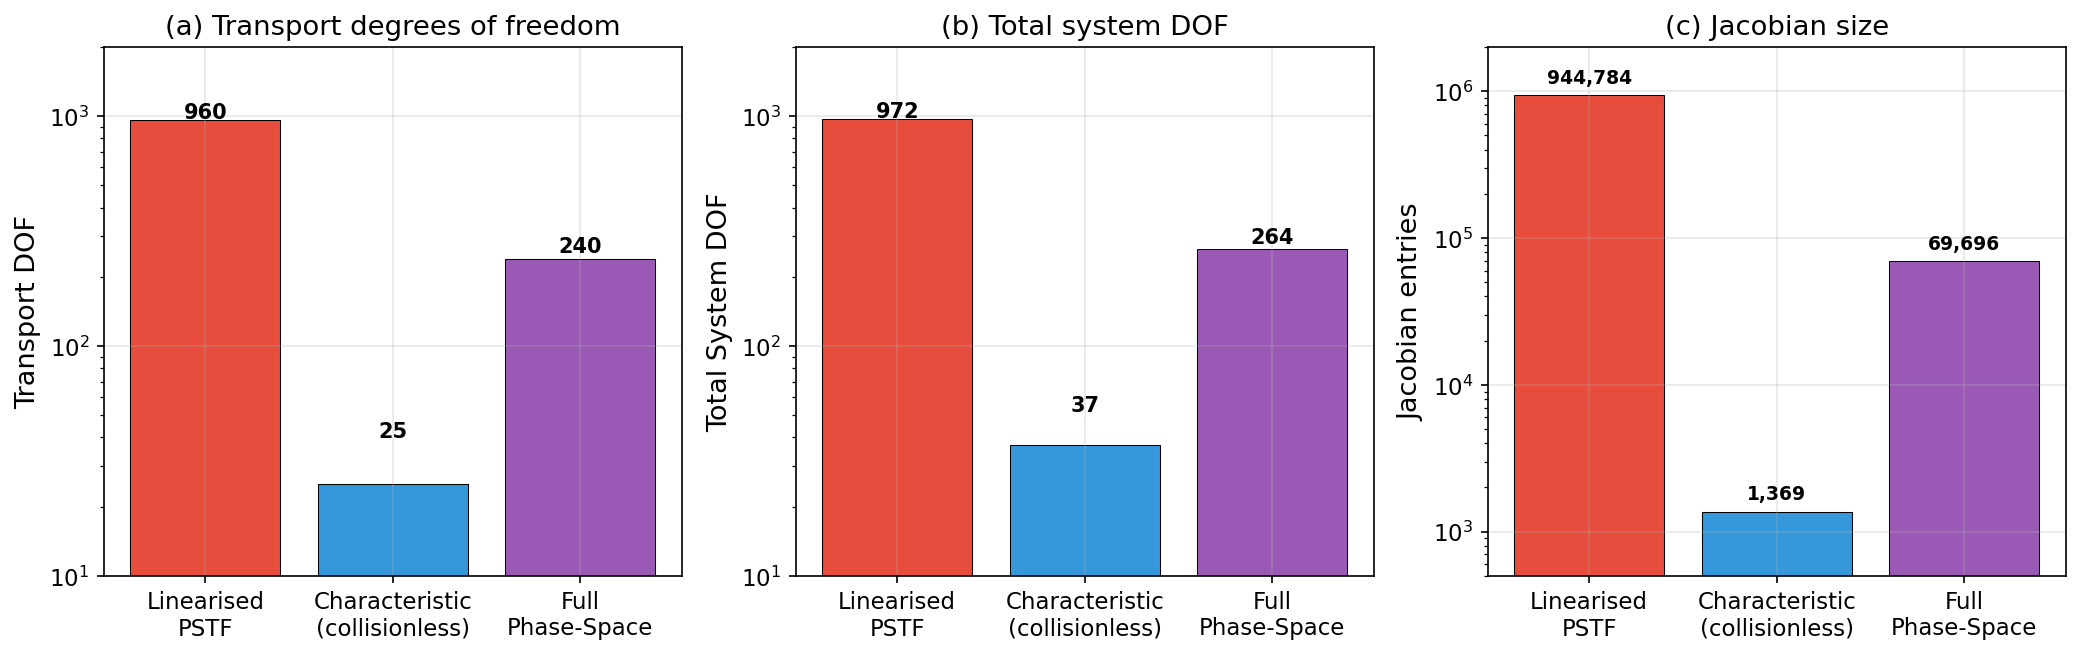
\includegraphics[width=\textwidth]{fig_ped07_phase_space_comparison.png}
\caption{Degrees of freedom comparison across transport methods.  (a)~Transport DOF: the linearised PSTF hierarchy requires 960 DOF, while characteristic rays need only 25.  The proposed full phase-space layout uses 240.  (b)~Indicative total system DOF including geometry and network.  (c)~Dense Jacobian entry count scales quadratically; the $\sim70{,}000$-entry estimate does not by itself establish Rosenbrock endpoint tractability.}\label{fig:dof_comparison}
\end{figure}

%======================================================================



\part{Production Pipeline}
\section{\texorpdfstring{Weak $n \leftrightarrow p$ Interconversion Rates}{Weak n<->p Interconversion Rates}}\label{sec:weak}
%======================================================================

\subsection{The Six Channels}

The six weak processes governing the neutron-to-proton ratio are:
\begin{align}
\text{(a)}\quad &\nu_e + n \to p + e^- && (\text{neutrino capture})\,,\\
\text{(b)}\quad &e^+ + n \to p + \bar\nu_e && (\text{positron capture})\,,\\
\text{(c)}\quad &n \to p + e^- + \bar\nu_e && (\text{neutron decay})\,,\\
\text{(d)}\quad &\bar\nu_e + p \to n + e^+ && (\text{anti-neutrino capture})\,,\\
\text{(e)}\quad &e^- + p \to n + \nu_e && (\text{electron capture})\,,\\
\text{(f)}\quad &p + e^- + \bar\nu_e \to n && (\text{inverse neutron decay})\,.
\end{align}

Channels (a)--(c) convert neutrons to protons ($\lambda_{n\to p}$), while (d)--(f) convert protons to neutrons ($\lambda_{p\to n}$).  In chemical equilibrium, detailed balance gives $\lambda_{p\to n}/\lambda_{n\to p} = e^{-Q/T}$ where $Q = m_n - m_p = 1.2933\;\mathrm{MeV}$, yielding the equilibrium neutron fraction $X_n^{\rm eq} = 1/(1 + e^{Q/T})$.

\subsection{Matrix Element and Phase Space}

The tree-level matrix element for neutron $\beta$-decay (channel~c) in the $V$--$A$ theory is
\begin{equation}
|\mathcal{M}|^2 = 2\,\GF^2\,(1 + 3g_A^2)\,,
\end{equation}
where $g_A = 1.2764$ is the axial coupling constant (PDG 2024).  For channel~(a), $\nu_e + n \to p + e^-$, the rate per neutron is:
\begin{equation}
\lambda^{(a)} = \frac{(1 + 3g_A^2)\,\GF^2}{2\pi^3}\int_{m_e}^\infty \dd\epsilon_e\;\epsilon_e\,p_e\,\epsilon_\nu^2\;\tilde{f}_{\nu_e}(\epsilon_\nu)\,[1 - f_e(\epsilon_e)]\,,\label{eq:lambda_a}
\end{equation}
where $\epsilon_\nu = \epsilon_e + Q$ (energy conservation, neglecting recoil), $p_e = \sqrt{\epsilon_e^2 - m_e^2}$, $\tilde{f}_{\nu_e}$ is the electron neutrino monopole distribution, and $f_e = [e^{\epsilon_e/T_\gamma} + 1]^{-1}$ is the electron Fermi--Dirac distribution.

The normalization constant $K = (1+3g_A^2)\,\GF^2/(2\pi^3)$ is fixed by requiring that the total decay rate equals $1/\tau_n$ when integrated over the free-neutron phase space:
\begin{equation}
\frac{1}{\tau_n} = K\int_{m_e}^{Q} \dd\epsilon_e\;\epsilon_e\,p_e\,(Q-\epsilon_e)^2\,,
\end{equation}
where the upper limit $Q$ reflects the maximum electron energy in neutron decay.  This integral gives $I_0 = 1.636$ (at Born level), fixing $K$.

\subsection{Live Rates as Distribution Functionals}

The critical feature of RABBIT's weak-rate implementation is that the rates are computed as \emph{live functionals} of the actual neutrino distribution $\tilde{f}_0(q)$, not of an assumed equilibrium Fermi--Dirac.  In the integrand \eqref{eq:lambda_a}, $\tilde{f}_{\nu_e}(\epsilon_\nu)$ is the momentum-dependent monopole from either the characteristic transport (capturing spectral distortion from anisotropy) or from the collision-evolved distribution (capturing incomplete decoupling).

This is essential for two reasons:
\begin{enumerate}
\item \textbf{Anisotropic Channel~2}: the spectral distortion $\tilde{f}_0(q) \neq f_{\rm FD}(q)$ from the anisotropic energy shift modifies the weak-rate integrands, producing the $\sim$1.4\% spectral contribution to $\Delta\Yp$.
\item \textbf{Incomplete decoupling}: the non-equilibrium neutrino spectrum from $e^\pm$ annihilation heating modifies the weak rates, contributing to the $\Neff = 3.044$ correction.
\end{enumerate}

\subsection{Correction Level Hierarchy}

Four correction levels are implemented in the current code base, though the historical reference figures in this report stop at CL2:

\begin{description}
\item[CL0 (Born):] Tree-level matrix element $|\mathcal{M}|^2 \propto (1 + 3g_A^2)\,\GF^2$.  The normalization integral is $I_0 = 1.636$.

\item[CL1 (+Coulomb):] The Sommerfeld Fermi function accounts for the Coulomb interaction between the outgoing proton/electron:
\begin{equation}
F(Z, \epsilon) = \frac{2\pi\eta}{e^{2\pi\eta} - 1}\,,\qquad \eta = \alpha Z/\beta\,,
\end{equation}
where $\beta = p_e/\epsilon_e$ and $Z = \pm 1$ for proton/electron final states.  This raises $I_0$ by $+3.40\%$.

\item[CL2 (+Sirlin radiative):] $\order(\alpha)$ virtual and real photon corrections via the Sirlin $g$-function:
\begin{equation}
1 + \frac{\alpha}{2\pi}\,g(\epsilon_e, Q)\,,
\end{equation}
applied multiplicatively to each channel.  Combined with Coulomb: $+4.95\%$.

\item[CL3 (+finite-mass / recoil / weak magnetism):] the current canonical code also supports the next weak-kernel layer beyond the historical CL2 presentation of this report.  In repository language this is the ``finite-mass'' or weak-budget layer: recoil, weak-magnetism, and related finite-mass corrections are carried as an additional multiplicative refinement on top of CL2.  The present report retains CL0--CL2 as its main figure language because the historical constraint plots were generated on that reference surface.
\end{description}

The historical FLRW baseline helium fractions quoted in this report at the CL0--CL2 levels are:
\begin{center}
\begin{tabular}{lccc}
\toprule
CL & $\Yp^{\rm FLRW}$ & D/H $\times 10^5$ & $\Neff$ \\
\midrule
0 (Born) & 0.24235 & 2.489 & 3.011 \\
1 (+Coulomb) & 0.24633 & 2.511 & 3.011 \\
2 (+Sirlin) & 0.24803 & 2.520 & 3.011 \\
\bottomrule
\end{tabular}
\end{center}

%======================================================================


\section{QED Equation of State}\label{sec:qed}
%======================================================================

The electromagnetic plasma at $T \lesssim 1\;\mathrm{MeV}$ receives QED corrections from $e^+e^-$ loop effects.  RABBIT uses the Bennett exact result at $\order(e^2) + \order(e^3)$ \cite{Bennett2020}:
\begin{equation}
\delta\rho_{\rm QED}/\rho_\gamma \approx -0.6\%\quad\text{(negative: reduces energy density at freeze-out).}
\end{equation}

The QED corrections affect BBN primarily through the photon--electron--positron equation of state: they modify $\rho(T)$, $p(T)$, and $s(T)$, which enter the Hubble rate and the $T_\gamma$ evolution.  The effect on $\Yp$ is $\delta\Yp \approx +3 \times 10^{-4}$.

The photon + $e^\pm$ plasma energy density, pressure, and entropy density are computed from the exact 1-loop effective potential, including:
\begin{itemize}
\item The free electron mass shift $\delta m_e^2 = (e^2/4\pi)\,T^2/3$ (thermal mass).
\item The photon self-energy (Debye screening).
\item The $\order(e^3)$ ring-diagram resummation (non-perturbative at $T \sim m_e$).
\end{itemize}

%======================================================================


\section{Nuclear Network}\label{sec:network}
%======================================================================

RABBIT tracks 9 nuclear species: n, p, D, T, $^3$He, $^4$He, $^7$Li, $^7$Be, $^6$Li.  The backbone network consists of 12 reactions from the PRIMAT AC2024 compilation, with an optional extension to 31 reactions including $^6$Li production channels.

Integration proceeds in two phases:
\begin{enumerate}
\item \textbf{Weak freeze-out} ($T: 10 \to 0.08\;\mathrm{MeV}$): only $n \leftrightarrow p$ interconversion is active.  The nuclear network is inactive, and abundances are set by NSE.
\item \textbf{Nuclear burning} ($T: 0.08 \to 0.005\;\mathrm{MeV}$): the full network is activated with NSE handoff initial conditions.
\end{enumerate}

%======================================================================


\section{Solver Architecture}\label{sec:solver}
%======================================================================

\subsection{Two stiff-solver families}

The current code base maintains two stiff-solver families with different roles.
\begin{enumerate}
\item \textbf{SciPy reference family:} the Type~I reference path uses \texttt{scipy.integrate.solve\_ivp} with Radau as the primary validation oracle and BDF as a stiffness comparison path.  This is the conservative reference / fallback backend in the current repository.
\item \textbf{JAX canonical family:} the bounded JAX Type~I surfaces use a native 8-stage Rodas5P implementation based on the Steinebach tableau \cite{Steinebach2023},
\begin{equation}
\left(\frac{\mathbf{I}}{\gamma h} - \mathbf{J}\right)\mathbf{k}_i
= \mathbf{f}\!\left(\mathbf{y}_n + \sum_{j<i} a_{ij}\,\mathbf{k}_j\right)
 \sum_{j<i} c_{ij}\frac{\mathbf{k}_j}{h},
\qquad \gamma = 0.21194\,,
\end{equation}
with runtime policy and Jacobian strategy chosen by the JAX driver metadata contracts.
\end{enumerate}

Fixed-step Rosenbrock is now retained only as a test-local native-AD smoke helper, not as a package-level runtime solver module or authority for the current canonical Type~I surfaces.

\subsection{Backend interpretation and current authority}

The old ``SciPy only'' hierarchy is no longer the right repository-level summary.  The current code distinguishes:
\begin{itemize}
\item \textbf{default reference surface:} \texttt{backend="auto"} / \texttt{"scipy"};
\item \textbf{explicit bounded JAX surface:} \texttt{backend="jax"};
\item \textbf{explicit exact-characteristic surfaces:} \texttt{backend="jax\_characteristic"} and \texttt{"jax\_characteristic\_tier2"};
\item \textbf{explicit higher-tier bounded surface:} \texttt{backend="jax\_advanced"} without Teff.
\end{itemize}

The report's historical figures remain attached to the exact-characteristic reference chain.  Any timing or backend statement should therefore be read together with its \emph{physics surface}: matched-physics parity statements are meaningful, mixed-surface timing comparisons are not.

\begin{figure}[t]
\centering
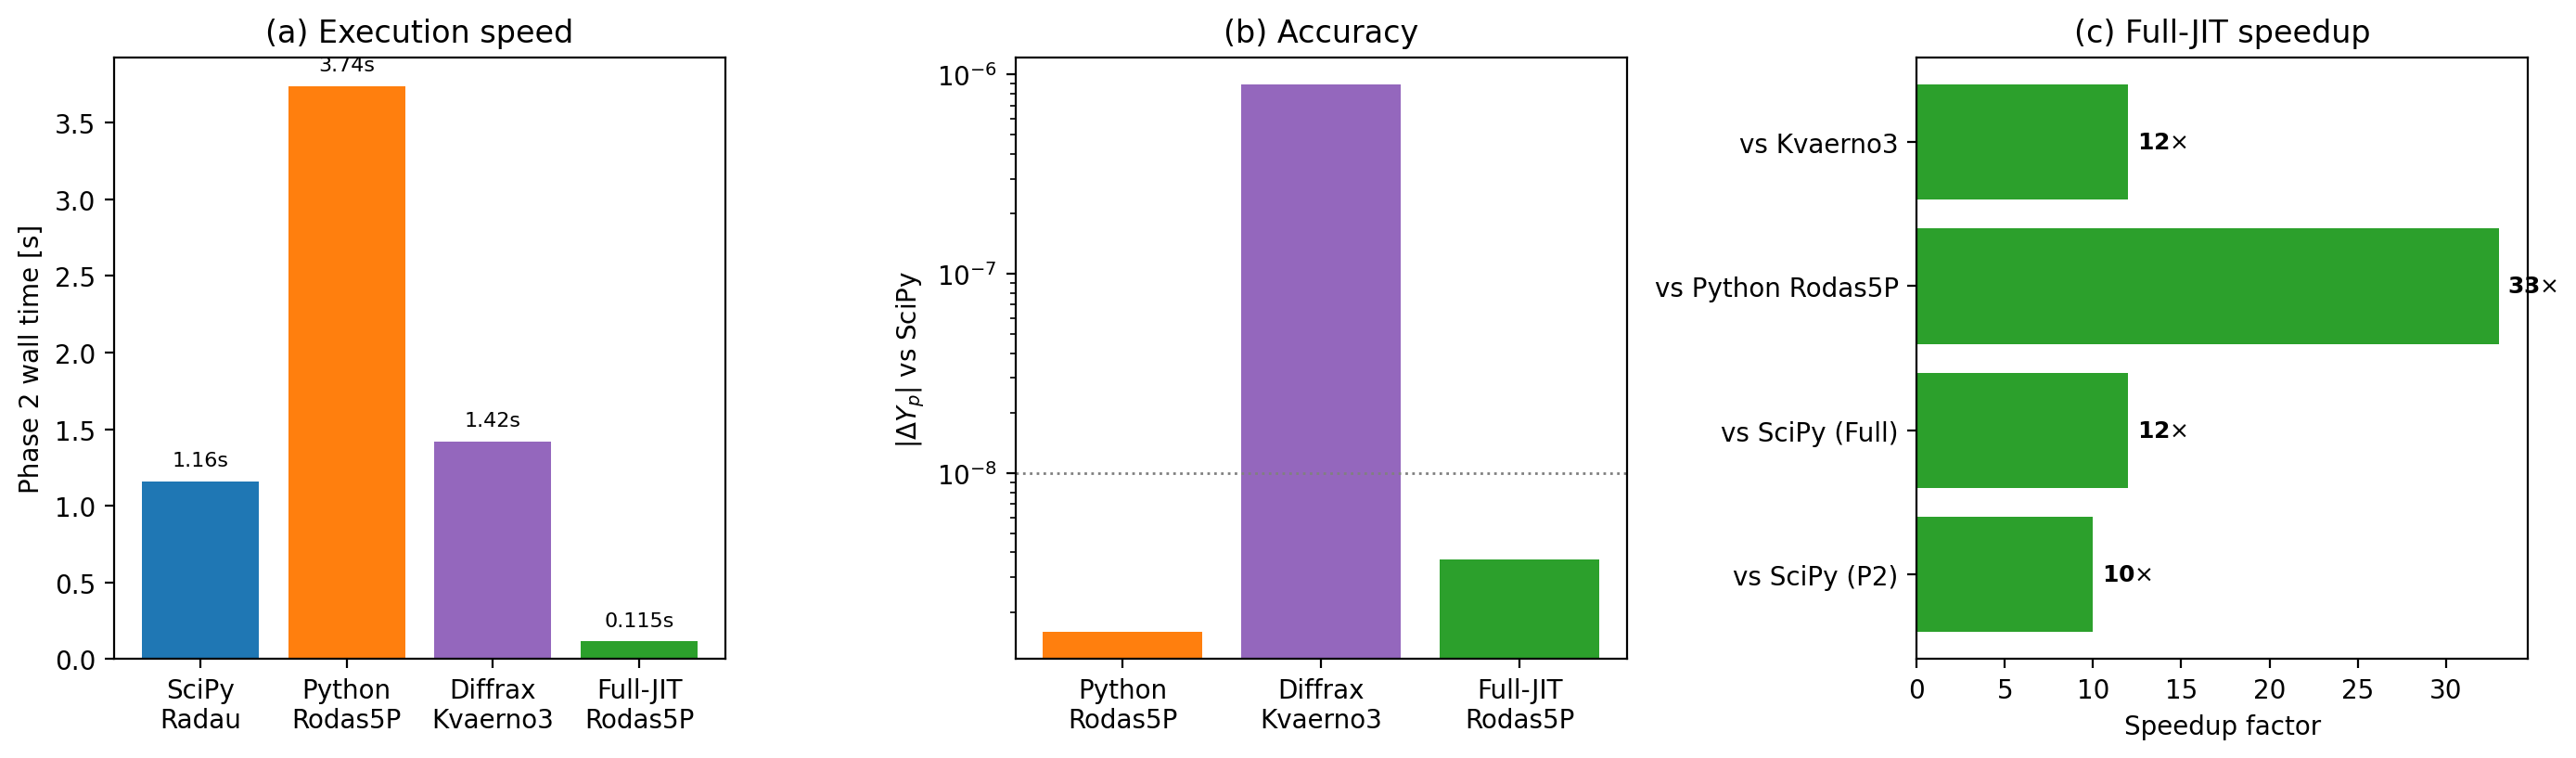
\includegraphics[width=\textwidth]{fig10.png}
\caption{Illustrative solver comparison.  The figure should now be read as a qualitative architecture sketch for the current solver families: SciPy implicit reference solves and JAX-native Rodas5P canonical surfaces.  The former fixed-step diagnostic AD probe is test-local only, not a runtime solver family.  This is not a current matched-physics benchmark table.}
\label{fig:solver}
\end{figure}

\subsection{Representative state vectors}

No single state vector now describes the entire canonical Type~I code scope.  The most important surfaces are:
\begin{enumerate}
\item \textbf{SciPy exact-characteristic reference layout:}
\begin{equation}
\mathbf{y}_{\rm SciPy,char}
= \bigl(\Sigma_+,\Sigma_-,I_{1\ldots12},J_{1\ldots12},S,T_\gamma,X_{0\ldots8}\bigr),
\end{equation}
which gives 37 total DOF at tier~1.
\item \textbf{JAX exact-characteristic compact layout:}
\begin{equation}
\mathbf{y}_{\rm JAX,char}
= \bigl(\Sigma_+,\Sigma_-,S,T_\gamma,X_{0\ldots8}\bigr)
\end{equation}
at tier~1, i.e.\ 13 total DOF; tier~2 adds $(T_{\nu_e},T_{\nu_x})$ for 15 total DOF.  The passive ray variables $I_j$ and $J_j$ are reconstructed analytically.
\item \textbf{JAX bounded default live-weak layout:}
\begin{equation}
\mathbf{y}_{\rm JAX,main}
= \bigl(\Sigma_+,\Sigma_-,\Psi_{\rm flat},T_\gamma,X_i\bigr),
\end{equation}
which is a large linearised PSTF state (972 total DOF at phase~2, tier~1, $N_q=80$).
\end{enumerate}

These are different numerical realisations with different scope contracts; they should not be conflated into a single ``production state vector'' statement.

%======================================================================


\section{The Full Coupled System}\label{sec:coupled}
%======================================================================

\subsection{Current scope declaration}

The historical figures in this report trace the mixed-closure exact-characteristic reference chain
\begin{equation}
(\Sigma,\Pi_\nu)\ \longrightarrow\ (\text{exact characteristic rays})\ \longrightarrow\ \tilde f_0(q)\ \longrightarrow\ (\lambda_{n\to p},\lambda_{p\to n})\ \longrightarrow\ X_i\,.
\end{equation}
In current code this exact-characteristic chain appears in two numerical forms: an explicit SciPy reference representation storing $(I_j,J_j,S)$, and a compact JAX characteristic representation evolving only $S$ and reconstructing $I_j$, $J_j$, and $\mu_j$ analytically.  The repository also ships bounded linearised live-weak JAX surfaces and a no-Teff tier~3 weak-budget surface; those are part of current code scope, but they are not identical to the exact-characteristic figures quoted later.  None of these paths constitutes a full anisotropic collision-coupled Boltzmann/QKE closure.

\subsection{Two production coupling channels}

The anisotropy affects BBN through two distinct but coupled channels:

\textbf{Channel 1 (expansion-rate enhancement):}
\begin{equation}
H = \frac{H_\FLRW}{\sqrt{1 - \Sigma^2}}\,.
\end{equation}
This accelerates the expansion, shifts weak freeze-out earlier, and raises $\Yp$.

\textbf{Channel 2 (monopole distortion):}
The exact characteristic monopole $\tilde f_0(q) \neq f_{\rm FD}(q)$ modifies the weak-rate integrands.  This effect is numerically subdominant to Channel~1, but it is not negligible at the precision level relevant for the historical reference constraint reported in this document.

\subsection{RHS evaluation order}

The right-hand side evaluation in the exact-characteristic reference chain proceeds in the following order:
\begin{enumerate}
\item unpack the current state vector;
\item reconstruct the current ray bundle, either from explicit $(I_j,J_j,S)$ variables or from the compact $S$-only state;
\item compute the characteristic stress tensor from the reconstructed rays;
\item evaluate the geometry RHS, including $\dd\Sigma_+/\dd N$;
\item advance the characteristic transport state: explicit $(I_j,J_j,S)$ on the SciPy reference path, or $S$ alone with analytic $I_j(S)$ and $J_j(S)$ reconstruction on the compact JAX characteristic path;
\item construct the reference-path thermodynamic closure for the Hubble sector (tier~1 baseline for the historical figures, with optional tier~2 extension hooks on the broader current-code surfaces);
\item extract the weak-rate monopole $\tilde f_0(q)$ from the rays;
\item evaluate the live weak rates $\lambda_{n\to p}[\tilde f_0]$ and $\lambda_{p\to n}[\tilde f_0]$;
\item compute the Hubble rate and plasma thermodynamics;
\item evaluate the nuclear-network RHS and repack the derivative.
\end{enumerate}

\begin{figure}[t]
\centering
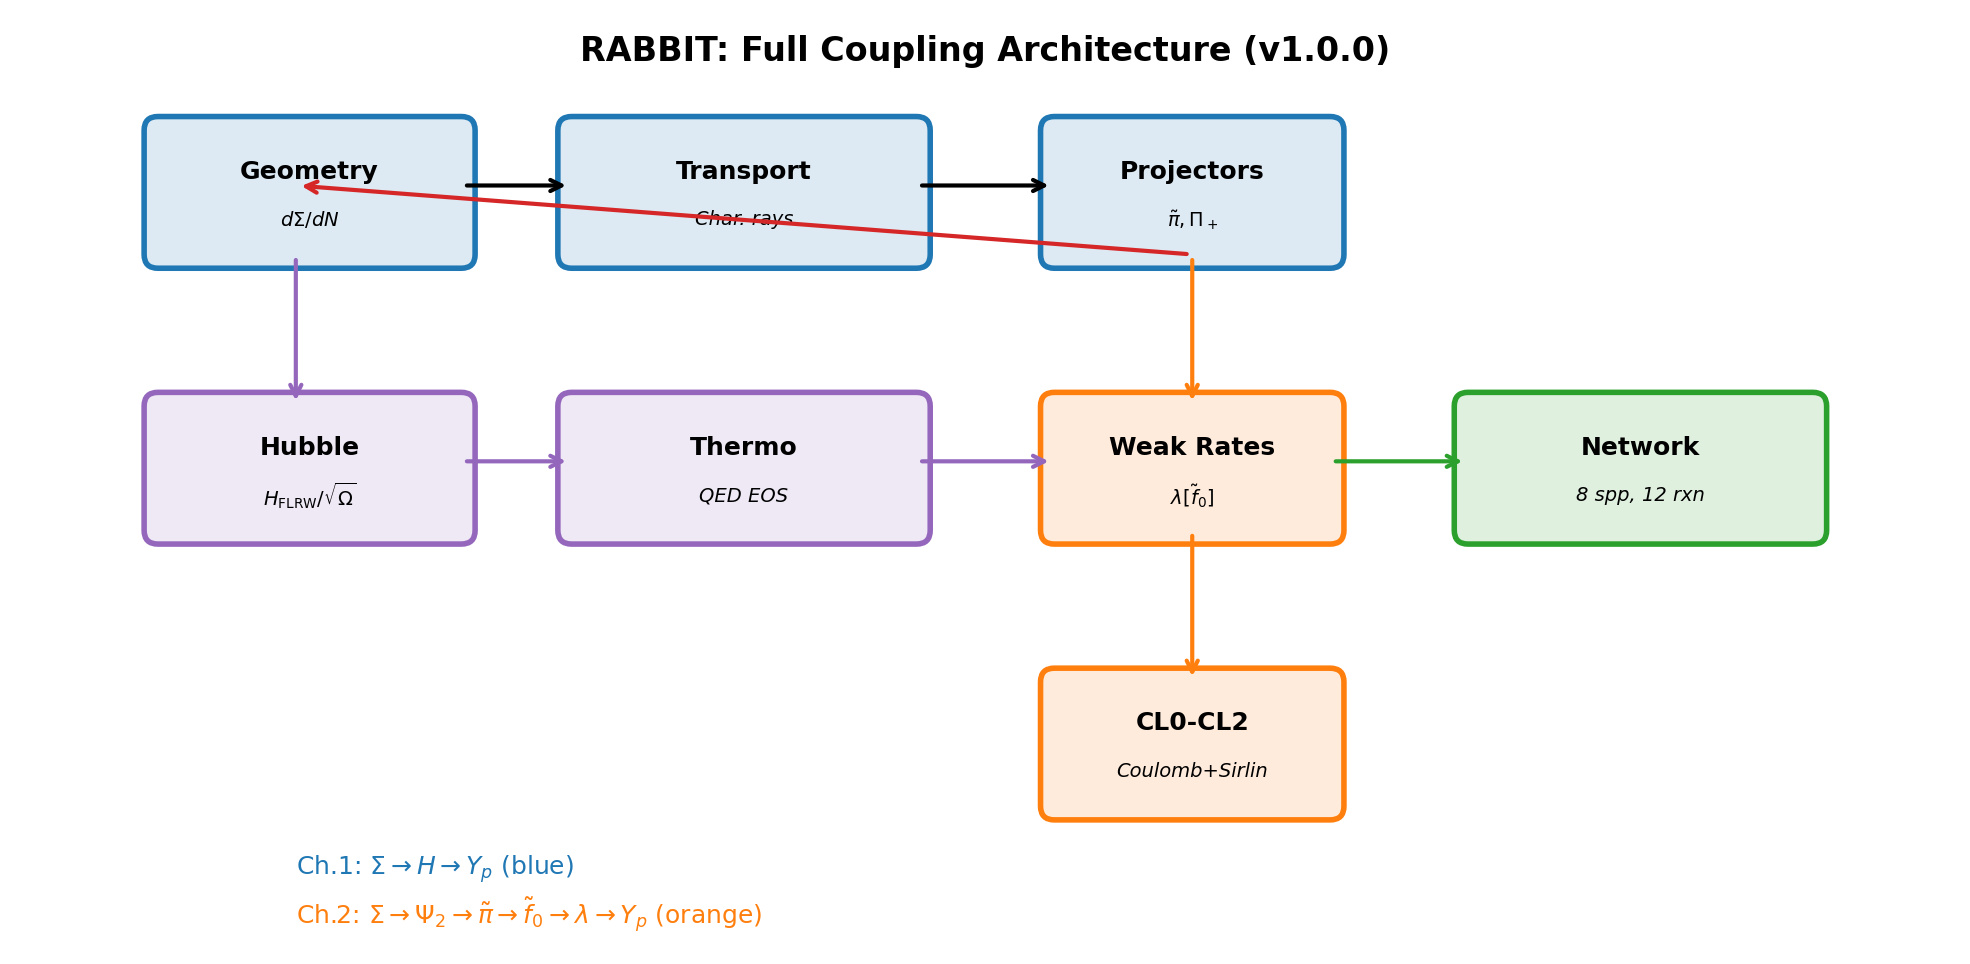
\includegraphics[width=\textwidth]{fig09.png}
\caption{Reference exact-characteristic code architecture.  The figure is a software-facing schematic of the mixed geometry--transport--weak--network solve that underlies the report's main figures.  Current code scope is broader than this single chain, but optional Teff or broader collision infrastructure should still be read as provenance or extension scaffolding rather than as part of the same maturity class as the historical exact-characteristic results.}
\label{fig:architecture}
\end{figure}

\begin{figure}[t]
\centering
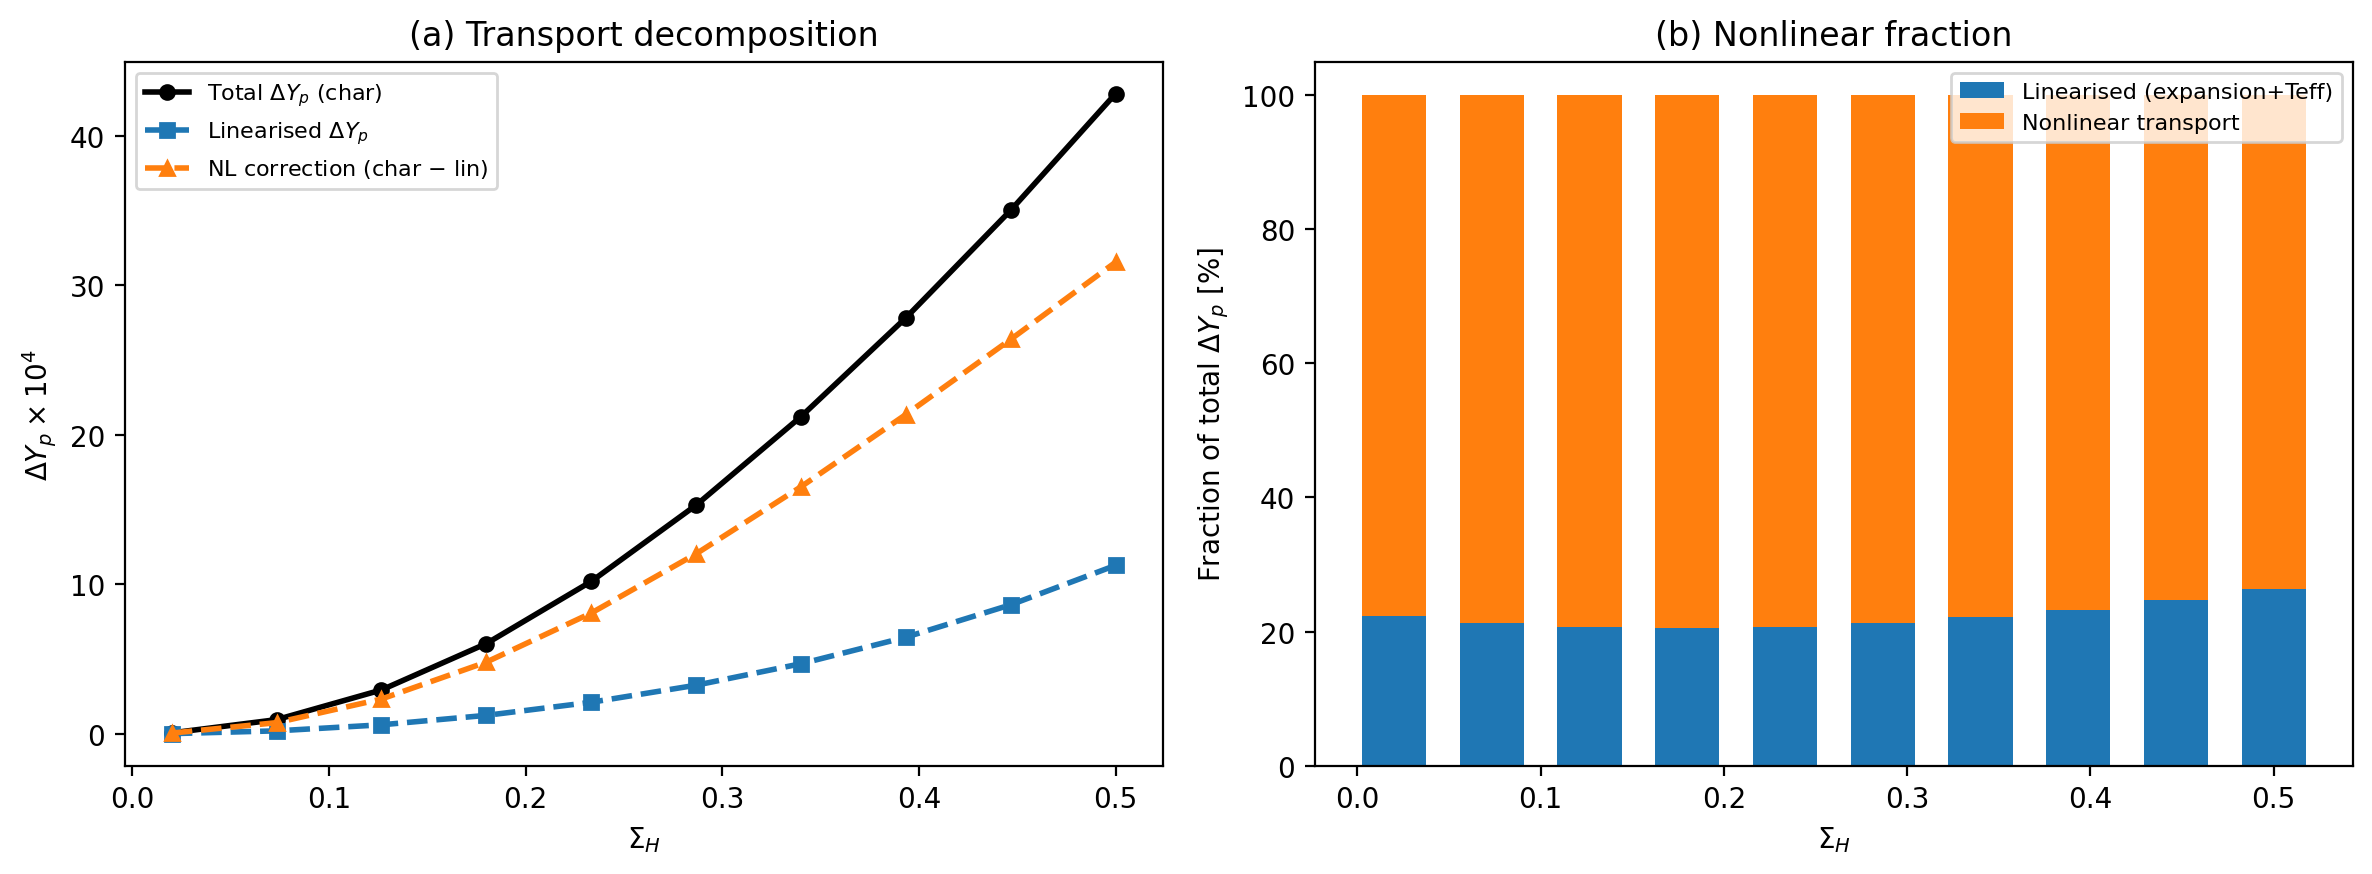
\includegraphics[width=\textwidth]{fig07.png}
\caption{Channel decomposition.  Panel~(a) separates the expansion-driven and distribution-driven contributions to $\Delta\Yp$; panel~(b) shows their fractions as a function of $\Sigma_H$.  The figure is intended as a decomposition diagnostic for the production path rather than as an additional independent constraint figure.}
\label{fig:channels}
\end{figure}

%======================================================================


\section{Results}\label{sec:results}
%======================================================================

\subsection{Geometry-to-transport backbone}

The results in this section are best read as a chain rather than as a bag of summary plots.  They correspond to the exact-characteristic reference chain discussed earlier, not to every current canonical backend equally.  In the current code base, the same figures should be understood as reference-path results reproduced by matched exact-characteristic JAX surfaces and contextualised relative to the broader JAX-first default envelope.

The geometry figure in \S\ref{sec:geometry} illustrates the first step of that historical diagnostic chain: a time-dependent interaction between the shear, the Hubble enhancement, and the neutrino anisotropic stress.  The next step is the transport-to-weak bridge.  The characteristic rays accumulate a direction-dependent energy shift, and the diagnostic monopole is obtained by ray quadrature rather than by a momentum-independent linearised closure.  These plots predate the publication programme's B-03/B-05 validation and are not current finite-shear evidence.

\begin{figure*}[t]
\centering
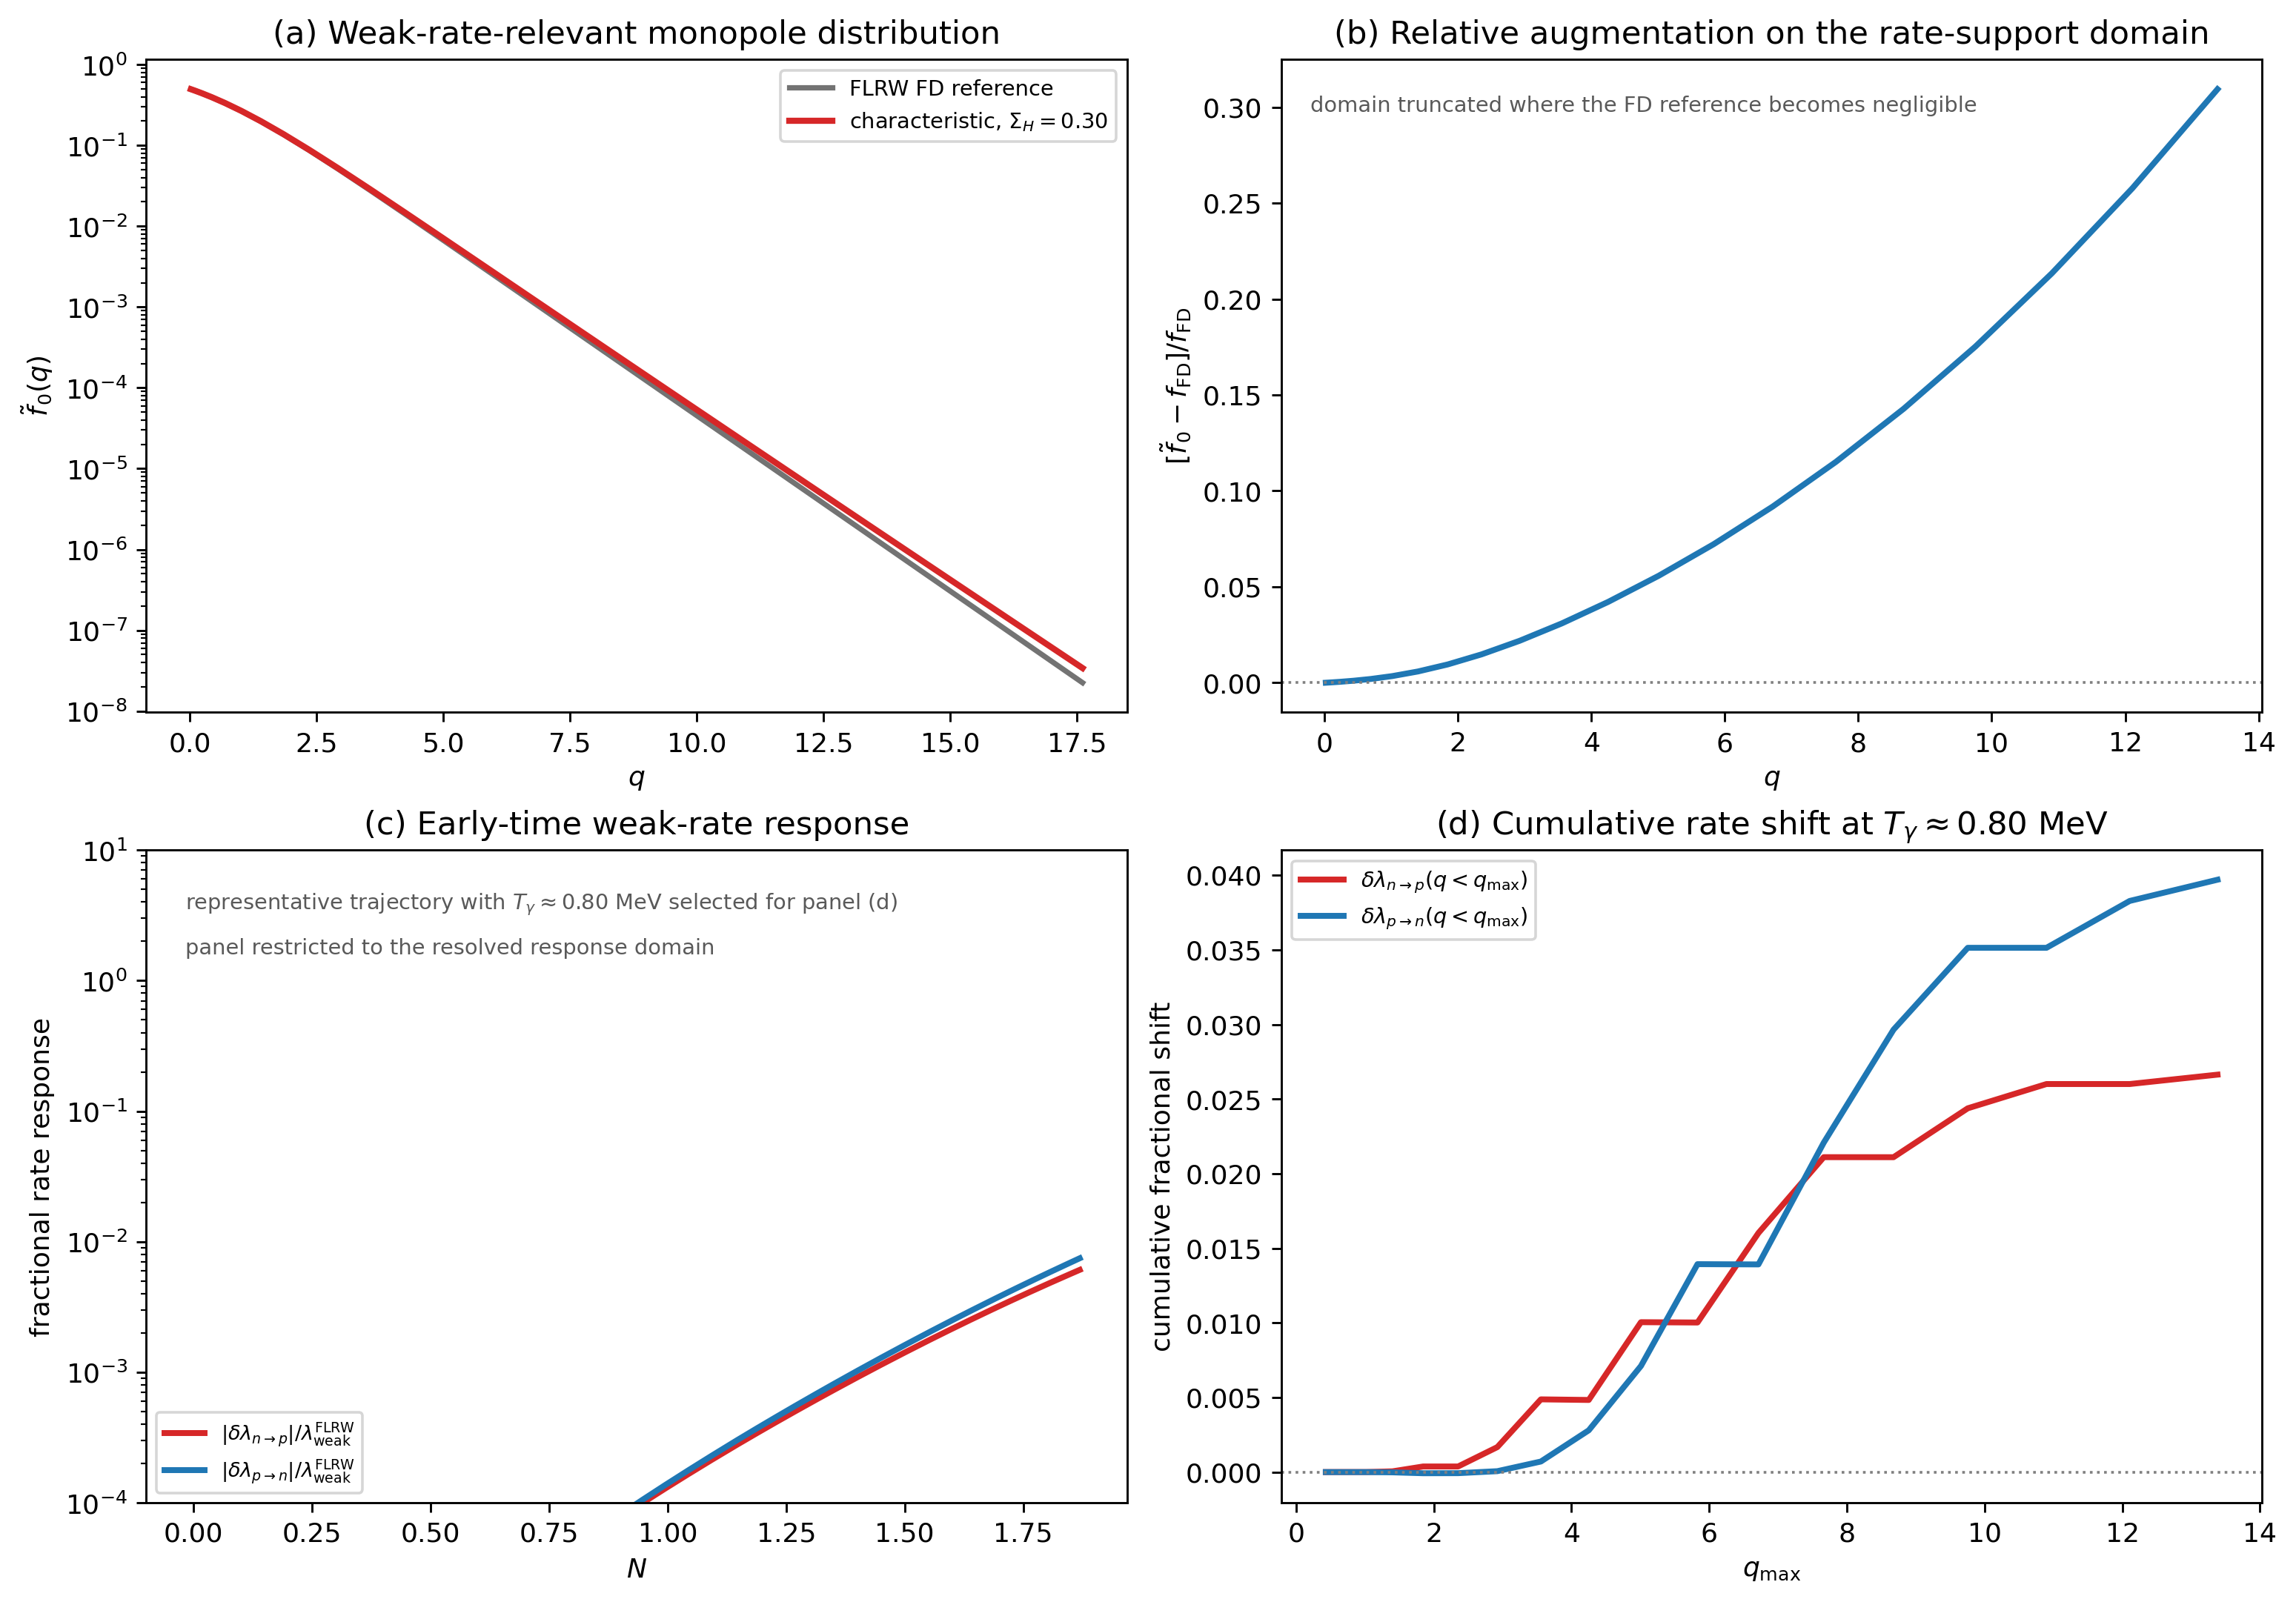
\includegraphics[width=\textwidth]{figures/fig_story_distribution_weak_bridge.png}
\caption{Bridge from the augmented monopole to the weak rates.  (a) The characteristic solution produces a weak-rate-relevant monopole $\tilde f_0(q)$ that is harder than the FLRW Fermi--Dirac reference.  (b) The relative augmentation grows toward the high-$q$ rate-support domain.  (c) The resulting perturbation induces a finite weak-rate response on the resolved early-time domain relevant for freeze-out.  (d) Integrating over momentum shows a cumulative fractional shift in $\lambda_{n\to p}$ and $\lambda_{p\to n}$ at the representative epoch $T_\gamma \simeq 0.80$ MeV.  Together these panels exhibit the middle link between characteristic transport and the final BBN-yield shift.}
\label{fig:story_bridge}
\end{figure*}

The central lesson of Fig.~\ref{fig:story_bridge} is that the characteristic method matters not merely because it produces a different quadrupole, but because it changes the weak-rate-relevant monopole itself.  The distortion is small at low momentum and grows across the rate-support domain, so the weak kernels are probed by a harder spectrum than the FLRW reference.  That is the physically important middle link between anisotropic transport and the observable BBN response.

\subsection{Direct BBN yield response}

\begin{table}[t]
\centering
\caption{BBN yields vs $\Sigma_H$ (CL2, characteristic transport, $\eta = 6.104 \times 10^{-10}$, $\tau_n = 878.4\,\mathrm{s}$).}\label{tab:yields}
\begin{tabular}{ccccc}
\toprule
$\Sigma_H$ & $\Yp$ (char) & $\Yp$ (lin) & $\Delta\Yp^{\rm NL}$ & D/H $\times 10^5$ \\
\midrule
0    & 0.24803 & 0.24803 & ---                   & 2.520 \\
0.10 & 0.24817 & 0.24807 & $+9.8\times 10^{-5}$  & 2.521 \\
0.30 & 0.24926 & 0.24839 & $+8.7\times 10^{-4}$  & 2.528 \\
0.50 & 0.25126 & 0.24917 & $+2.1\times 10^{-3}$  & 2.541 \\
\bottomrule
\end{tabular}
\end{table}

The resulting yield response is monotonic in $\Sigma_H$: increasing anisotropy raises $\Yp$ and, more weakly, D/H.  The nonlinear correction $\Delta\Yp^{\rm NL}$ grows super-linearly because the momentum-dependent spectral remapping is itself nonlinear in the accumulated characteristic energy shift.

\begin{figure*}[t]
\centering

\includegraphics[width=\textwidth]{figures/fig18.png}
\caption{Historical diagnostic BBN response to anisotropic expansion.  The panels show legacy CL2 outputs for $Y_p$ and D/H as functions of $\Sigma_H$, together with observational bands and the FLRW reference.  The dashed vertical line is a legacy runtime guard, not a validated physical-domain boundary.  The figure does not establish a publication constraint; B-03 and B-05 remain open.}
\label{fig:observable_response}
\end{figure*}

\subsection{Historical profile-likelihood diagnostic (not validated)}

Using $\Yp^{\rm obs} = 0.2449 \pm 0.0040$ (Aver et al.) and $(\mathrm{D/H})^{\rm obs} = (2.547 \pm 0.029) \times 10^{-5}$ (Cooke et al.), the legacy Type~I CL2 grid emitted a numerical crossing near $\Sigma_H=0.66$.  That value is a \textbf{DEPRECATED diagnostic readout}, not a validated confidence bound, and must not be cited as a current science result.  A finite-shear domain and canonical likelihood are not validated until B-03 and B-05 pass.

\begin{figure*}[t]
\centering
\includegraphics[width=\textwidth]{figures/fig21.png}
\caption{Historical diagnostic likelihood structure for the legacy Type~I grid.  Panel~(a) shows $\Delta\chi^2(\eta_{10},\Sigma_H)$ and reference contour levels; panel~(b) shows the corresponding profile statistic.  Neither the $0.75$ runtime guard nor the crossing is a validated publication domain or constraint.}
\label{fig:chi2}
\end{figure*}

At Born level the legacy FLRW baseline lay slightly low in $\Yp$, while Coulomb and Sirlin corrections shifted that diagnostic comparison.  No preference or bound from this scan is promoted by the current publication programme; the canonical inference path is deferred to B-05.

%======================================================================


\section{Inference and Gradient Bridge}\label{sec:inference}
%======================================================================

For the historical Type~I diagnostic grid we used the abundance-level chi-squared
\begin{equation}
\chi^2(\eta_{10},\SigH)=\sum_a \frac{\bigl(\mathcal O_a^{\rm th}(\eta_{10},\SigH)-\mathcal O_a^{\rm obs}\bigr)^2}{\sigma_a^2}\,,
\end{equation}
with $a\in\{\Yp,\mathrm{D/H}\}$ for the present grid illustrations, i.e. $\mathcal O_a$ denotes the abundance observables rather than a species mass-fraction label.  The displayed contour figure uses the shifted quantity
\begin{equation}
\Delta\chi^2(\eta_{10},\SigH)=\chi^2(\eta_{10},\SigH)-\chi^2_{\min}
\end{equation}
and the corresponding one-dimensional diagnostic is the profile statistic
\begin{equation}
\Delta\chi^2_{\rm prof}(\SigH)=\min_{\eta_{10}}\Delta\chi^2(\eta_{10},\SigH)\,.
\end{equation}
These definitions explain Fig.~\ref{fig:chi2}.  The following stored finite-difference numbers are historical diagnostics only; the retired host-solver custom-VJP is fail-closed and no BBN-specific JAX sampler is publication-authoritative before B-05.  At the old fiducial point:
\begin{align}
\frac{\partial\log\mathcal{L}}{\partial\eta_{10}} &= -44.09\,,\\
\frac{\partial\log\mathcal{L}}{\partial\tau_n} &= +0.114\,.
\end{align}

The old sensitivity ratio and grid morphology may guide future test design, but they do not validate a likelihood surface or a shear constraint.  Figure~\ref{fig:chi2} is therefore a historical diagnostic visualisation only.  The $\SigH=0.75$ line is a legacy runtime guard rather than a validated physical boundary, and B-03/B-05 must establish both the domain and the canonical full-solver likelihood.

\begin{figure}[t]
\centering
\includegraphics[width=\textwidth]{fig21.png}
\caption{Historical diagnostic likelihood grid in the $(\eta_{10},\SigH)$ plane.  The contour thresholds and profile curve are retained for provenance, not as a current confidence construction.  The $\SigH=0.75$ line is a legacy runtime guard; the finite-shear publication domain and inference result remain NOT VALIDATED pending B-03/B-05.}\label{fig:chi2_inference}
\end{figure}

%======================================================================


\section{Validation}\label{sec:validation}
%======================================================================

\subsection{FLRW recovery}

At $\Sigma = 0$ the characteristic and linearised transport paths agree to $|\Yp^{\rm char} - \Yp^{\rm lin}| < 7 \times 10^{-10}$ across all CL levels.  This verifies that the characteristic method exactly recovers FLRW when anisotropy vanishes.

\subsection{PRIMAT cross-validation}

At Born level with PRIMAT parameters ($\tau_n = 879.4\,\mathrm{s}$, $\eta = 6.10 \times 10^{-10}$), RABBIT gives $\Yp = 0.24255$ compared with the PRIMAT anchor $0.24248$, giving $|\Delta\Yp| = 6.7 \times 10^{-5}$.  Figure~\ref{fig:primat} summarises the FLRW helium values across the correction hierarchy and the adopted PRIMAT anchor; panel~(b) is an accounting visual rather than a microscopic source decomposition.

\begin{figure}[t]
\centering
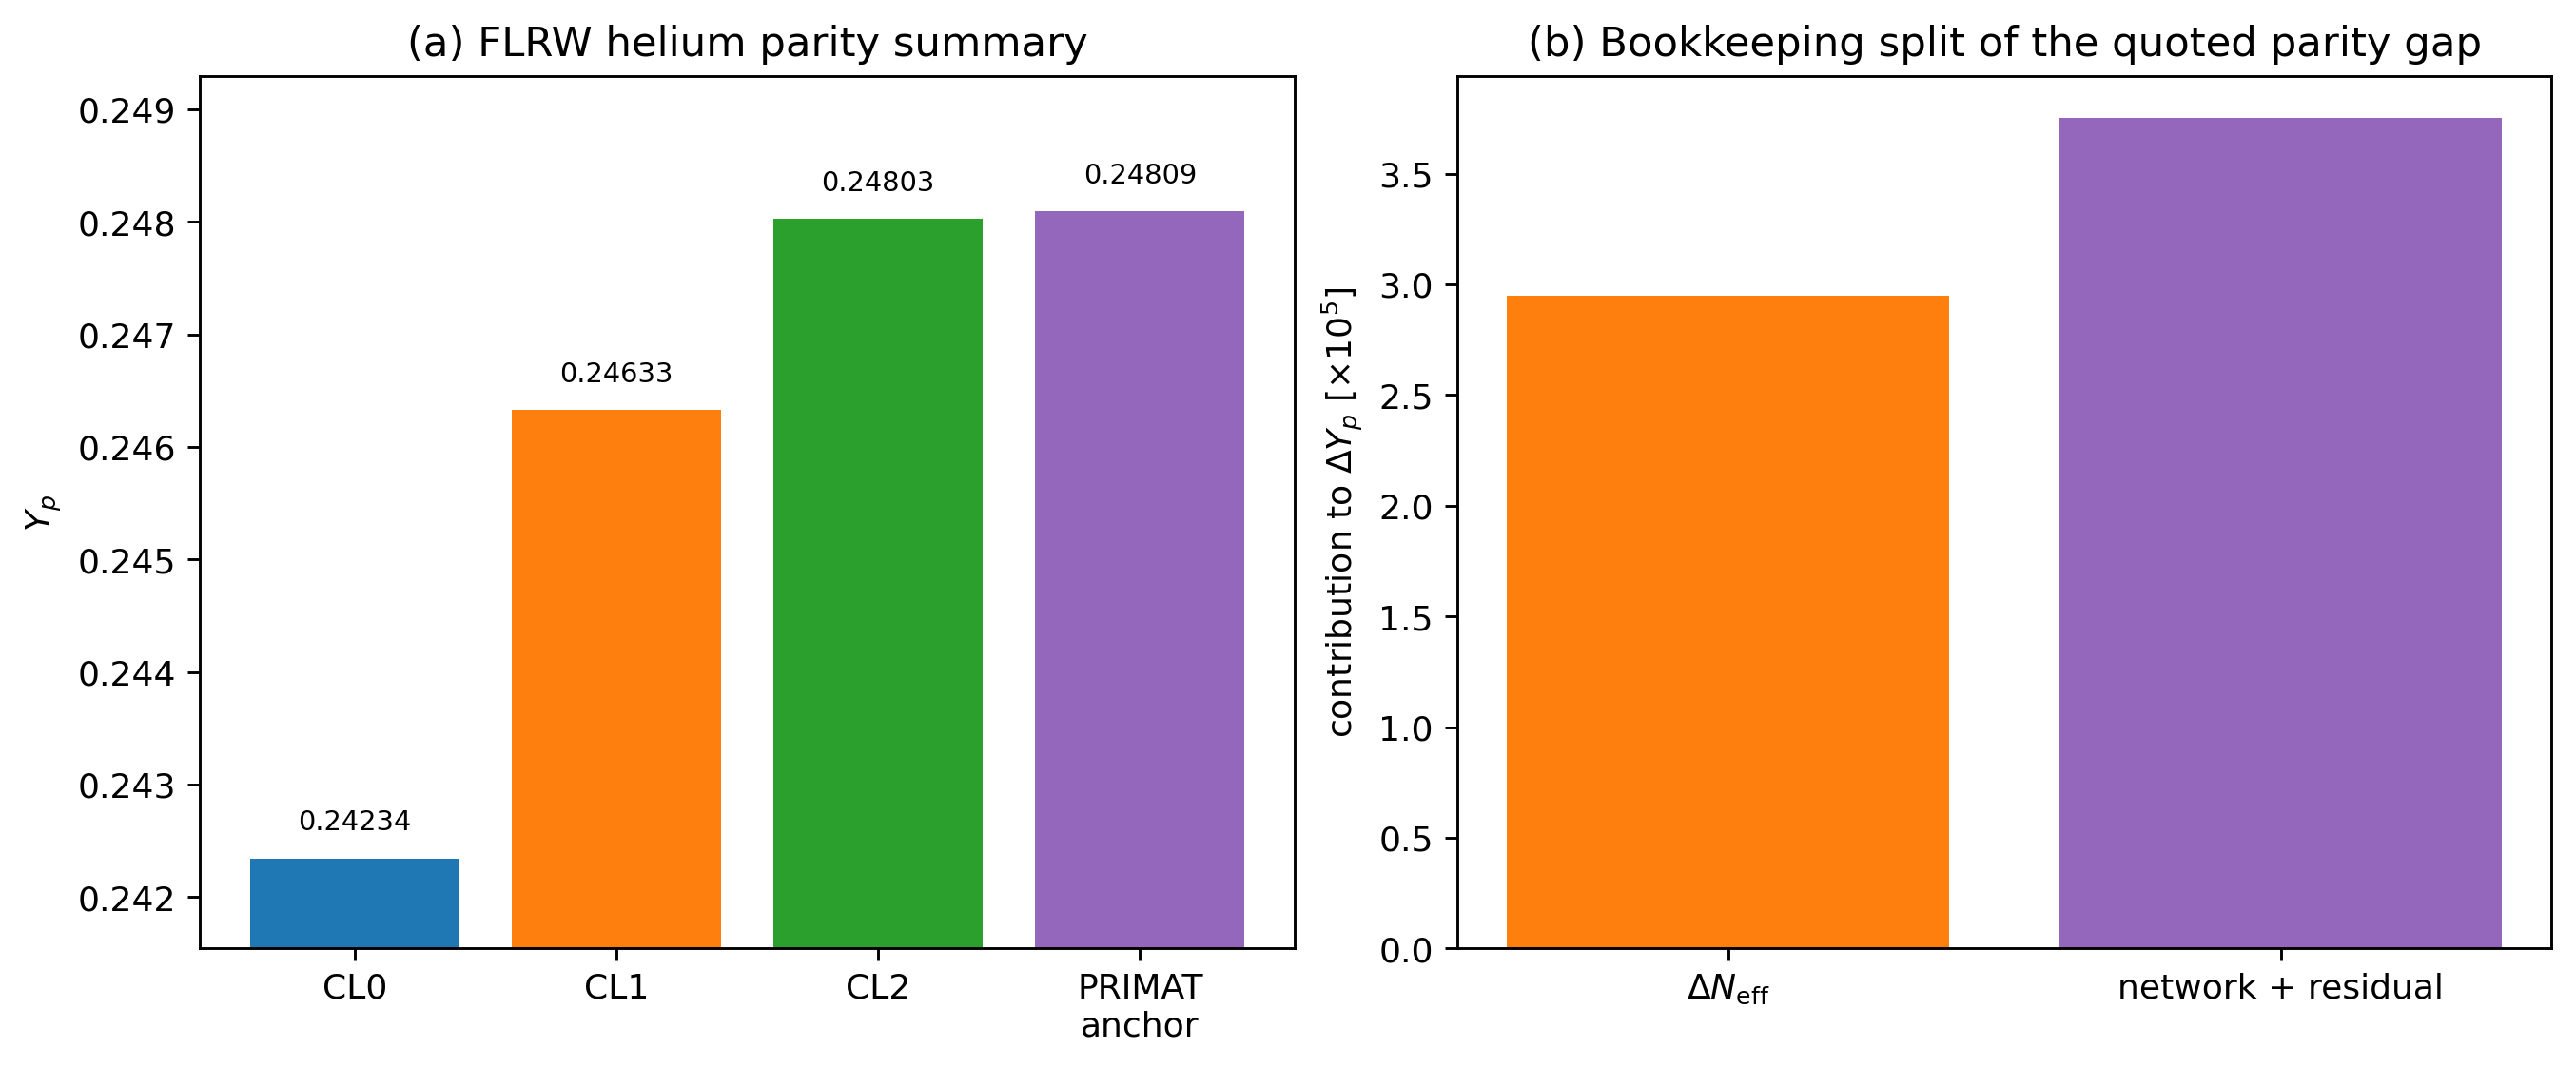
\includegraphics[width=\textwidth]{figures/fig19.png}
\caption{FLRW helium cross-validation summary.  (a) Reported $\Yp$ values for the CL0, CL1, and CL2 weak-rate hierarchies together with the PRIMAT anchor used for the parity check.  (b) Bookkeeping decomposition of the enforced headline parity $|\Delta\Yp| = 6.7 \times 10^{-5}$ into a $\Delta\Neff$-like share and a residual network/calibration share.  Panel~(b) is an accounting visualisation rather than a first-principles microscopic source decomposition.}
\label{fig:primat}
\end{figure}

\subsection{SciPy--JAX parity on the current canonical Type~I surfaces}

Current code scope is broader than the original SciPy-only framing of this report.  The exact-characteristic JAX driver is now parity-locked against the SciPy characteristic reference on matched tier~1 and tier~2 cells, and the bounded JAX default / advanced surfaces are regression-checked against corresponding SciPy cells on their declared envelopes.  These are numerical-consistency claims about the current code surfaces, not separate new physics results distinct from the reference figures shown elsewhere in this report.

\subsection{Convergence and discretisation checks}

The characteristic production path must also pass a simpler numerical question: are the reported yield shifts stable under the chosen ray and momentum resolutions?  Figure~\ref{fig:convergence} shows the baseline-relative discretisation diagnostics at $\Sigma_H=0.3$.  The point of the figure is not to fit a universal asymptotic law at every sampled quadrature, but to demonstrate that the adopted production resolution lies in the numerically stable region of the scan.

\begin{figure}[t]
\centering

\includegraphics[width=\textwidth]{figures/fig16.png}
\caption{Characteristic transport convergence at $\Sigma_H = 0.3$.  (a) Angular convergence of the helium yield with increasing characteristic-ray resolution $N_\mu$, shown as $|\Delta\Yp|\times 10^5$ relative to the baseline production run.  (b) Momentum-resolution diagnostic with increasing quadrature size $N_q$, again relative to the same baseline.  Both panels are baseline-relative discretisation checks rather than separate physics results.}
\label{fig:convergence}
\end{figure}

\subsection{What is and is not validated here}

The current tests support runtime-regression statements about FLRW recovery, stored PRIMAT comparison cells, characteristic-ray discretisation, and matched SciPy--JAX execution.  They do not independently validate the underlying finite-shear physics, a matched external BBN anchor, or the historical profile crossing.  Those publication claims remain blocked by B-01--B-06, and a fully anisotropic collision-coupled decoupling solver is outside the present claim ceiling.

%======================================================================


\section{Discussion}\label{sec:discussion}
%======================================================================

\subsection{What the characteristic correction is really telling us}

The nonlinear transport correction is not a cosmetic detail.  The characteristic route changes the weak-rate-relevant monopole through a momentum-dependent remapping of the phase space, and the resulting hardening is one of the reasons the exact characteristic path cannot be replaced by the momentum-independent linearised closure when quoting production BBN constraints.  The key message is therefore not simply that the quadrupole differs, but that the production monopole entering the live weak kernels differs in a way that integrates to a measurable yield shift.

\subsection{Limitations and outlook}

The limitations that matter for the present report are best stated in the same reference/bounded/deferred language used in \S\ref{sec:incomplete_decoupling}.
\begin{enumerate}
\item \textbf{Reference-result baseline:} the quoted Type~I characteristic figures are anchored to the exact-characteristic reference chain with tier~1 thermodynamic closure, CL0/CL1/CL2 weak figures, Bennett QED EOS, and the PRIMAT network.
\item \textbf{Bounded current-code surfaces:} tier~1 JAX default, exact-characteristic JAX tier~1/tier~2, and the no-Teff JAX tier~3 weak-budget surface are real canonical code surfaces, but each is valid only on its declared backend envelope and none should be confused with a full anisotropic collision solver.
\item \textbf{Out of scope:} full QKE, fully anisotropic collision-coupled Boltzmann evolution, complete $\nu$--$\nu$ plus $\nu$--$e$ angular closure, and the candidate Class~A / Class~B / tilted perimeter as headline production claims.
\item \textbf{Inference scope:} the present report documents the explicit Type~I likelihood surface and profile constraint.  Broader sampler and evidence machinery exist in the repository, but they are not the source of the headline figures here.
\end{enumerate}

The most durable scientific contribution of the present document is therefore the clarified exact-characteristic Type~I story itself: geometry, exact characteristic transport, monopole distortion, weak-rate response, and observable BBN constraint.  Everything beyond that chain should be read either as a bounded current-code surface with its own scope contract, or as extension scaffolding, validation support, or deferred future work rather than as part of the same maturity class as the historical headline figures.

%======================================================================


\section{Conclusions}\label{sec:conclusions}
%======================================================================

RABBIT v1.0.0, as documented here in its current Type~I code scope, delivers:

\begin{enumerate}
\item A current canonical Type~I core that spans a SciPy reference / fallback path, a bounded JAX-first tier~1 default surface, explicit exact-characteristic JAX tier~1 and tier~2 surfaces, and a bounded no-Teff JAX tier~3 weak-budget surface.

\item Historical exact-characteristic diagnostic outputs---the shear envelope, nonlinear yield response, and legacy profile crossing---retained for provenance and future falsification, not promoted as current science results.

\item A clarified distinction between \emph{physics representation} and \emph{numerical state contract}: the SciPy characteristic reference path keeps explicit $(I_j,J_j,S)$ ray variables, while the compact JAX characteristic path reconstructs $I_j$ and $J_j$ analytically from $S$.

\item A tiered incomplete-decoupling hierarchy in which tier~1 anchors the historical figures, tier~2 characteristic three-temperature thermo is a bounded canonical extension, and the no-Teff tier~3 weak-budget ladder is implemented as a bounded canonical JAX surface, without claiming a full anisotropic collision-coupled Boltzmann/QKE closure.

\item A runtime-regression posture covering FLRW recovery cells, stored PRIMAT comparisons, characteristic convergence, and bounded SciPy--JAX parity, without treating self-consistency as publication validation.

\item A code-to-formula account of the exact-characteristic reference chain together with an honest description of the broader current code scope and its boundaries.
\end{enumerate}

Everything beyond that scope---including a finite-shear science result, candidate perimeter geometries, Bayes-factor experimentation, and full anisotropic collision-coupled decoupling---is unvalidated or deferred future work.

%======================================================================



\begin{appendices}
\section{Physical Constants}\label{app:constants}
%======================================================================

\begin{table}[tbp]
\centering
\caption{Physical constants and observational values.}
\begin{tabular}{lcl}
\toprule
Quantity & Value & Source \\
\midrule
$\tau_n$ & $878.4 \pm 0.5\;\mathrm{s}$ & PDG 2024 \\
$\eta$ & $(6.104 \pm 0.058) \times 10^{-10}$ & Planck 2018 \\
$\Neff^{\rm SM}$ & 3.044 & PDG 2024 \\
$Q_{np}$ & $1.2933\;\mathrm{MeV}$ & PDG 2024 \\
$G_N$ & $6.709 \times 10^{-45}\;\mathrm{MeV}^{-2}$ & PDG 2024 \\
$\GF$ & $1.1664 \times 10^{-11}\;\mathrm{MeV}^{-2}$ & PDG 2024 \\
$\sw$ & 0.23122 & PDG 2024 ($\overline{\rm MS}$) \\
$m_e$ & $0.5110\;\mathrm{MeV}$ & PDG 2024 \\
$f_\nu$ & 0.4052 & Standard 3$\nu$ \\
$\Yp^{\rm obs}$ & $0.2449 \pm 0.0040$ & Aver et~al.\ 2021 \\
$(\mathrm{D/H})^{\rm obs}$ & $(2.547 \pm 0.029) \times 10^{-5}$ & Cooke et~al.\ 2018 \\
\bottomrule
\end{tabular}
\end{table}

%======================================================================


\section{Canonical Eigenvalue Values}\label{app:eigenvalue_table}
%======================================================================

\begin{table}[tbp]
\centering
\caption{Canonical eigenvalue and coupling constants (v1.0.0, corrected).}
\begin{tabular}{lcc}
\toprule
Quantity & Value & System \\
\midrule
$\lambda_{\rm slow}$ & $-0.687$ & $(\Sig, \tilde\pi)$ reduced \\
$\lambda_{\rm fast}$ & $-4.313$ & $(\Sig, \tilde\pi)$ reduced \\
$\mathrm{Re}(\lambda)$ & $-1/2$ (exact) & $(\Sig, \Psi_2)$ transport \\
$\omega$ & $1.023\;\mathrm{rad/e\text{-}fold}$ & $(\Sig, \Psi_2)$ transport \\
$D$ & 4 & Quadrupole damping \\
$C_{\rm fb}$ & $24/5 = 4.8$ & Feedback coefficient \\
$C_{\rm src}$ & $8/15 \approx 0.533$ & Source coefficient \\
$C_{\rm drain}$ & 4 & Drain coefficient \\
$f_\nu$ & 0.4052 & Neutrino fraction \\
$\mathrm{tr}(\mathbf{M})$ & $-5$ (universal) & Both systems \\
$\det(\mathbf{M})$ & 2.963 & Reduced system \\
$|\tilde\pi|/|\Sig|$ attractor & 0.133 & Quasi-static \\
\bottomrule
\end{tabular}
\end{table}

%======================================================================


\section{Weak Coupling Constants}\label{app:weak_couplings}
%======================================================================

\begin{table}[tbp]
\centering
\caption{Standard Model weak couplings for neutrino--electron interactions.}
\begin{tabular}{lcccc}
\toprule
Species & $\GL$ & $\GR$ & $\GL^2 + \GR^2$ & $a_{\rm total}$ \\
\midrule
$\nu_e$ (CC+NC) & 0.731 & 0.231 & 0.588 & 2.353 \\
$\nu_\mu, \nu_\tau$ (NC) & $-0.269$ & 0.231 & 0.126 & 0.503 \\
\bottomrule
\end{tabular}
\end{table}

The coupling ratio $a_e/a_x \approx 4.68$ means electron neutrinos remain coupled to the plasma $\sim$5 times longer than muon and tau neutrinos, producing flavour-dependent spectral distortion during incomplete decoupling.

%======================================================================


\section{Code Architecture: Developer Reference}\label{app:code}

This appendix is a current-scope guide to the repository as it exists now.  It is \emph{not} a line-accurate record of every historical implementation path.  The single sources of truth for backend maturity and dispatch are \path{src/rabbit/config/backend_capabilities.py} and \path{src/rabbit/inference/forward_likelihood.py}; whenever this appendix and the code disagree, the code wins.

\subsection{Package Layout}

\begin{verbatim}
src/rabbit/
|-- config/        backend registry, transport/solver conventions, grids
|-- drivers/       SciPy Type-I reference + perimeter drivers
|-- geometry/      Bianchi geometry kernels and constraints
|-- inference/     canonical_forward_solver and likelihood wrappers
|-- jax/           JAX Type-I main, characteristic, advanced, Class A/B
|-- network/       PRIMAT AC2024 reaction tables + abundance RHS
|-- solver/        SciPy-side Rosenbrock utilities and solve_ivp helpers
|-- thermo/        tiered neutrino-decoupling / plasma EOS infrastructure
|-- transport/     characteristic rays, PSTF hierarchies, phase-space extension helpers
|-- validation/    parity, truncation, and production-fence utilities
`-- weak/          live weak-rate quadratures and correction layers
\end{verbatim}

\subsection{Canonical Type~I Surfaces}

The repository's current Type~I core is broader than the original SciPy-only framing of the report.  The current public surfaces are:

\begin{center}
\renewcommand{\arraystretch}{1.12}
\begin{tabularx}{0.97\textwidth}{@{}p{0.20\textwidth}p{0.18\textwidth}p{0.16\textwidth}X@{}}
\toprule
Public backend & Transport & Thermo & Current role \\
\midrule
\texttt{auto} / \texttt{scipy} & exact characteristic & tier~1 reference (tier~2/3 candidates exist separately) & default SciPy Type~I reference \\
\texttt{jax} & linearised PSTF + live weak & tier~1 & explicit bounded JAX Type~I surface \\
\texttt{jax\_characteristic} & exact characteristic & tier~1 & explicit canonical exact-characteristic JAX surface \\
\texttt{jax\_characteristic\_tier2} & exact characteristic & tier~2 3T & explicit canonical characteristic 3T surface \\
\texttt{jax\_advanced} & linearised PSTF + live weak & tier~3 weak-budget, no Teff & bounded canonical higher-tier JAX surface \\
\bottomrule
\end{tabularx}
\end{center}

Candidate perimeters such as Class~A, Class~B, tilted models, and full anisotropic collision-coupled transport remain outside the headline Type~I claims of this report.

\subsection{Current Transport Surfaces}

\paragraph{SciPy Type~I reference path (\texttt{drivers/full\_coupled\_typeI.py}).}
This is the conservative Type~I reference / fallback backend.  It still carries the explicit characteristic-ray state $(I_j,J_j,S)$ when \texttt{transport\_mode=CHARACTERISTIC}, and it also houses the transitional tier~2 / tier~3 SciPy candidate paths.

\paragraph{JAX main Type~I path (\texttt{jax/driver\_typeI.py}).}
This explicit JAX surface is selected by \texttt{backend="jax"} or a recorded runtime opt-in.  It is not the \texttt{auto} default or publication authority.  Physically it is \emph{not} identical to the exact-characteristic reference chain: it uses the linearised Type~I transport surface and is tracked through metadata contracts.

\paragraph{JAX exact-characteristic path (\texttt{jax/driver\_typeI\_char.py}).}
This is the explicit JAX realization of the exact characteristic transport chain.  It mirrors the SciPy characteristic reference path on matched cells and carries two important current-scope contracts:
\begin{itemize}
\item \texttt{characteristic\_state\_contract="analytic\_intensity\_from\_shear\_map\_v1"}
\item CPU-first runtime execution with retry-on-CPU fallback metadata when GPU runtime instability is detected
\end{itemize}

\paragraph{Characteristic kernels (\texttt{transport/characteristic\_rays.py}, \texttt{jax/characteristic\_rays\_jax.py}).}
These modules carry the exact LRS ray formulas:
\begin{equation}
\mu_j(S)=\mathrm{sign}(\mu_{0,j})\sqrt{\frac{X_{0,j}e^{6S}}{1+X_{0,j}e^{6S}}},
\qquad
I_j(S)=\frac{1}{4}\ln\!\left[\frac{1+X_{0,j}e^{6S}}{1+X_{0,j}}\right]-\frac{S}{2},
\end{equation}
together with the analytic forward Jacobian $J_j(S)=\dd\mu_j/\dd\mu_{0,j}$ and the ray-to-monopole / ray-to-stress quadratures.

\subsection{Representative State Contracts}

The current repository no longer has a single canonical Type~I state layout.  The most important contracts are:
\begin{enumerate}
\item \textbf{SciPy exact-characteristic reference layout:}
\begin{equation}
\mathbf y_{\rm SciPy,char}
= \bigl(\Sigma_+,\Sigma_-,I_{1\ldots12},J_{1\ldots12},S,T_\gamma,X_{0\ldots8}\bigr),
\end{equation}
which is the old 37-DOF tier~1 reference layout.
\item \textbf{JAX exact-characteristic compact layout:}
\begin{equation}
\mathbf y_{\rm JAX,char}
= \bigl(\Sigma_+,\Sigma_-,S,T_\gamma,X_{0\ldots8}\bigr)
\end{equation}
at tier~1 (13 total DOF), or with $(T_{\nu_e},T_{\nu_x})$ inserted at tier~2 (15 total DOF).  The passive ray variables are reconstructed analytically.
\item \textbf{JAX bounded default live-weak layout:}
\begin{equation}
\mathbf y_{\rm JAX,main}
= \bigl(\Sigma_+,\Sigma_-,\Psi_{\rm flat},T_\gamma,X_i\bigr),
\end{equation}
which is a large linearised-PSTF state (972 total DOF at phase~2, tier~1, $N_q=80$).
\end{enumerate}

These state contracts correspond to different public surfaces and must not be collapsed into a single ``RABBIT state vector'' statement.

\subsection{Solver and Runtime Policy}

\paragraph{SciPy reference family.}
The SciPy reference path uses \texttt{solve\_ivp} with Radau as the primary validation oracle and BDF as a stiffness comparison path.  This is the conservative reference / fallback authority for Type~I.

\paragraph{JAX canonical family.}
The JAX Type~I surfaces use the native Rodas5P implementation in \path{jax/solver_jax_rodas5p.py}.  Runtime policy is CPU-first by default, and both the main JAX driver and the exact-characteristic JAX driver report runtime-device metadata such as:
\begin{itemize}
\item \texttt{runtime\_device\_policy}
\item \texttt{runtime\_device\_contract}
\item \texttt{runtime\_device\_fallback\_applied}
\end{itemize}

\paragraph{Auto dispatch.}
\texttt{canonical\_forward\_solver(..., backend="auto")} resolves to the SciPy Type~I reference.  JAX selection is explicit or requires a recorded opt-in; it is not publication authority.

\subsection{What This Appendix Does and Does Not Claim}

This appendix documents the current architecture honestly.
\begin{enumerate}
\item It \textbf{does} describe the current canonical Type~I surfaces and their numerical state contracts.
\item It \textbf{does} distinguish the historical exact-characteristic report figures from the broader current repository surface.
\item It \textbf{does not} claim that every canonical backend regenerates the historical figures in exactly the same way.
\item It \textbf{does not} claim a full anisotropic collision-coupled Boltzmann/QKE closure.
\item It \textbf{does not} upgrade Teff, Class~A / Class~B / tilted, or full phase-space ray ideas into headline production claims.
\end{enumerate}

The practical rule for a hostile audit is therefore simple: read the figures in the main text as exact-characteristic reference results, read \path{backend_capabilities.py} as the maturity registry for current code scope, and read metadata contracts on individual runs to determine which bounded surface actually produced a given prediction.


\section{Full Phase-Space Ray Boltzmann Equation}\label{app:full_ray}
%======================================================================

This appendix derives the full Boltzmann equation along characteristic rays when the state per ray is the complete distribution $f_j(q_k)$ rather than the single scalar $I_j$.  This is the deferred full phase-space formulation that eliminates reduced temperature-projection closures entirely.

\subsection{State Representation}

In the full phase-space approach, each of the $N_\mu$ rays carries $N_q$ distribution values:
\begin{equation}
\text{State per ray:}\quad f_j(q_1), f_j(q_2), \ldots, f_j(q_{N_q})\,,\qquad j = 1, \ldots, N_\mu\,.
\end{equation}

The total transport DOF is $N_\mu \times N_q$.  With $N_\mu = 12$ and $N_q = 20$: 240 DOF, compared to $2N_\mu + 1 = 25$ in the collisionless characteristic approach.

\subsection{Evolution Equation}

The Boltzmann equation along ray $j$ is:
\begin{equation}
\frac{\partial f_j(q)}{\partial N} = -\left(\frac{\dd\ln q}{\dd N}\right)_{\!j}\,q\,\frac{\partial f_j}{\partial q} + \frac{C[f](q, \mu_j)}{H}\,.\label{eq:full_ray_boltzmann}
\end{equation}

The gravitational redshift term $(\dd\ln q/\dd N)_j = -\Sig_+\,P_2(\mu_j)$ is the same as in the collisionless case.  The new ingredient is the collision term $C[f](q, \mu_j)/H$, which is evaluated directly at each momentum node and direction.

\subsection{Collision Coupling Between Rays}

The collision integral at direction $\mu_j$ requires knowledge of the distribution at \emph{all} directions (through the angular part of the matrix element).  In the full phase-space approach, this is handled by a direct angular gather, collision, and per-ray application cycle at each timestep, without reduced temperature compression:

\begin{enumerate}
\item \textbf{Gather}: construct the angle-averaged monopole and quadrupole from all rays:
\begin{align}
\tilde{f}_0(q) &= \frac{1}{2}\sum_j w_j\,J_j\,f_j(q)\,,\\
\tilde{f}_2(q) &= \frac{5}{2}\sum_j w_j\,J_j\,P_2(\mu_j)\,f_j(q)\,.
\end{align}

\item \textbf{Collide}: compute $C[f](q, \mu_j)$ using the monopole (and optionally quadrupole) projections:
\begin{equation}
C[f](q, \mu_j) = C_0[\tilde{f}_0](q) + C_2[\tilde{f}_0, \tilde{f}_2](q)\,P_2(\mu_j) + \order(\Sig^2)\,.
\end{equation}

\item \textbf{Apply}: add $C[f](q, \mu_j)/(H\,\Delta N)$ directly to each ray's distribution at each momentum node:
\begin{equation}
f_j(q_k) \to f_j(q_k) + \frac{C[f](q_k, \mu_j)}{H}\,\Delta N\,.
\end{equation}
\end{enumerate}

No temperature-projection step is needed: the collision effect is applied per-momentum, per-ray.  The spectral distortion from collisions is captured exactly (to the order of the multipole truncation of $C$).
\subsection{Advantages and Costs}

The full phase-space approach has several advantages over reduced temperature-projection closures:
\begin{itemize}
\item No scalar scatter approximation: the collision integral is applied directly at each $q$.
\item Spectral distortions from collisions (momentum-dependent rates) are captured exactly.
\item The state $f_j(q)$ can represent arbitrary distributions, not just boosted Fermi--Dirac.
\item Self-consistent incomplete decoupling: the evolved $f_j(q)$ naturally captures the $\Neff = 3.044$ correction.
\end{itemize}

The costs are:
\begin{itemize}
\item DOF increase: 25 $\to$ 240 (for $N_\mu = 12$, $N_q = 20$).
\item Jacobian size: $37^2 = 1{,}369 \to 264^2 \approx 70{,}000$ (still tractable for Rodas5P).
\item Memory: $\sim$3 KB $\to$ $\sim$20 KB per evaluation (negligible).
\item The $q$-derivative $q\,\partial f/\partial q$ requires careful numerical treatment (upwind schemes or spectral methods) to avoid Gibbs oscillations.
\end{itemize}

\subsection{Initial Conditions}

At $N = 0$ ($T = T_{\rm start} = 10\;\mathrm{MeV}$), all rays start with the equilibrium Fermi--Dirac distribution:
\begin{equation}
f_j(q_k, N=0) = f_{\rm FD}(q_k) = \frac{1}{e^{q_k} + 1}\,,\qquad \forall\,j\,.
\end{equation}

During the coupled phase ($T > T_{\rm dec}$), collisions maintain $f_j \approx f_{\rm FD}$ with small corrections.  After decoupling ($T < T_{\rm dec}$), collisions switch off and the evolution reduces to the characteristic solution $f_j(u, N) = f_{\rm FD}(u\,e^{2I_j})$.

This demonstrates that the collisionless characteristic approach is the correct \emph{asymptotic} solution after decoupling, and the full phase-space approach is needed only during the decoupling epoch itself.

\subsection{Implementation Status}

The full phase-space ray formulation is designed but not yet implemented in RABBIT.  The implementation requires:
\begin{enumerate}
\item Upgrading the driver state vector from $\{I_j\}$ to $\{f_j(q_k)\}$.
\item Implementing a stable $q$-advection scheme for the gravitational redshift term.
\item Wiring the collision operator to act per-ray, per-momentum.
\item Validating against known results (LASAGNA, FortEPiaNO) in the FLRW limit.
\end{enumerate}

This is the primary scope of Paper~II.

%======================================================================



\end{appendices}
\begin{thebibliography}{30}
\bibitem{WainwrightEllis1997} J.~Wainwright and G.~F.~R.~Ellis, \emph{Dynamical Systems in Cosmology} (Cambridge University Press, 1997).
\bibitem{Barrow1976} J.~D.~Barrow, Mon.\ Not.\ R.\ Astron.\ Soc.\ \textbf{175}, 359 (1976).
\bibitem{Misner1968} C.~W.~Misner, Astrophys.\ J.\ \textbf{151}, 431 (1968).
\bibitem{RothmanMatzner1982} T.~Rothman and R.~Matzner, Phys.\ Rev.\ Lett.\ \textbf{48}, 1565 (1982).
\bibitem{Planck2020anomalies} Planck Collaboration, Astron.\ Astrophys.\ \textbf{641}, A7 (2020).
\bibitem{Riess2022} A.~G.~Riess et~al., Astrophys.\ J.\ Lett.\ \textbf{934}, L7 (2022).
\bibitem{Secrest2022} N.~J.~Secrest et~al., Astrophys.\ J.\ Lett.\ \textbf{937}, L31 (2022).
\bibitem{PitrouPRIMAT2021} C.~Pitrou, A.~Coc, J.-P.~Uzan, E.~Vangioni, Mon.\ Not.\ R.\ Astron.\ Soc.\ \textbf{502}, 2474 (2021).
\bibitem{PArthENoPE2018} R.~Consiglio et~al., Comput.\ Phys.\ Commun.\ \textbf{233}, 237 (2018).
\bibitem{AlterBBN2020} A.~Arbey et~al., Comput.\ Phys.\ Commun.\ \textbf{248}, 106982 (2020).
\bibitem{Bennett2020} J.~J.~Bennett et~al., J.\ Cosmol.\ Astropart.\ Phys.\ \textbf{2020}(03), 003 (2020).
\bibitem{Steinebach2023} G.~Steinebach, BIT Numer.\ Math.\ \textbf{63}, 27 (2023).
\bibitem{Aver2021} E.~Aver, K.~A.~Olive, E.~D.~Skillman, J.\ Cosmol.\ Astropart.\ Phys.\ \textbf{2021}(03), 027 (2021).
\bibitem{Cooke2018} R.~J.~Cooke, M.~Pettini, C.~C.~Steidel, Astrophys.\ J.\ \textbf{855}, 102 (2018).
\bibitem{HannestadMadsen1995} S.~Hannestad and J.~Madsen, Phys.\ Rev.\ D \textbf{52}, 1764 (1995).
\bibitem{NotzoldRaffelt1988} D.~N\"otzold and G.~Raffelt, Nucl.\ Phys.\ B \textbf{307}, 924 (1988).
\bibitem{Mangano2005} G.~Mangano et~al., Nucl.\ Phys.\ B \textbf{729}, 221 (2005).
\bibitem{deSalas2016} P.~F.~de~Salas and S.~Pastor, J.\ Cosmol.\ Astropart.\ Phys.\ \textbf{2016}(07), 051 (2016).
\bibitem{Froustey2020} J.~Froustey, C.~Pitrou, M.~C.~Volpe, J.\ Cosmol.\ Astropart.\ Phys.\ \textbf{2020}(12), 015 (2020).
\bibitem{Dolgov1997} A.~D.~Dolgov et~al., Nucl.\ Phys.\ B \textbf{503}, 426 (1997).
\bibitem{Escudero2019} M.~Escudero, J.\ Cosmol.\ Astropart.\ Phys.\ \textbf{2019}(02), 007 (2019).
\end{thebibliography}


\end{document}
